% This template was originally by R. Jacob Vogelstein
% Updated on March 1, 2010 by Noah J. Cowan


%\documentclass[12pt,oneside,final]{thesis}
\documentclass[12pt]{report}

\pdfminorversion=5
\pdfobjcompresslevel=0
\usepackage[a-1b]{pdfx}

\usepackage{pdfpages}

\pagestyle{myheadings}
%\topmargin=0.25in
\topmargin=0.05in
\textheight=8.15in
\textwidth=5.6in
\oddsidemargin=0.7in
\raggedbottom
\newdimen \jot \jot=5mm
\brokenpenalty=10000
 

\usepackage[utf8]{inputenc}
%\DeclareUnicodeCharacter{00A0}{ }
\usepackage[T1]{fontenc}
\usepackage{lmodern} % load a font with all the characters
%\usepackage{hyperref}
\usepackage{tocbibind} % need this to contents adding for TOC
\usepackage{setspace}
\setstretch{1.05}
\usepackage{RJournal_nogeom}
%\usepackage[all]{hypcap}
\usepackage[hypcap=true]{caption}
\hypersetup{linktocpage}
\usepackage{amsmath,amssymb,array}
\usepackage{booktabs}
\usepackage{subfig}

%% load any required packages here
\usepackage{graphicx}
\usepackage{float}
\usepackage{tikz}
\usepackage{graphics} 
\usetikzlibrary{positioning}
\usetikzlibrary{shapes,arrows}
\usepackage{dcolumn}
\newcommand{\bbeta}{\mbox{\boldmath $\beta$}}

%%%%%%%%%%%%%%%%%%%%%%%%%%%%%%%%%%%%%%%%%%%%%%%%%%%%%%%%%%%%%%%%
% DOI from Segmentation
% Don't use - needs hyperref
%%%%%%%%%%%%%%%%%%%%%%%%%%%%%%%%%%%%%%%%%%%%%%%%%%%%%%%%%%%%%%%%
%\makeatletter
%\providecommand{\doi}[1]{%
%  \begingroup
%    \let\bibinfo\@secondoftwo
%    \urlstyle{rm}%
%    \href{http://dx.doi.org/#1}{%
%      doi:\discretionary{}{}{}%
%      \nolinkurl{#1}%
%    }%
%  \endgroup
%}
%\makeatother

%%%%%%%%%%%%%%%%%%%%%%%%%%%%%%%%%%%%%%%%%%%%%%%%%%%%%%%%%%%%%%%%
% StartKNITR STUFF
%%%%%%%%%%%%%%%%%%%%%%%%%%%%%%%%%%%%%%%%%%%%%%%%%%%%%%%%%%%%%%%%
\usepackage{color}
%% maxwidth is the original width if it is less than linewidth
%% otherwise use linewidth (to make sure the graphics do not exceed the margin)
\makeatletter
\def\maxwidth{ %
  \ifdim\Gin@nat@width>\linewidth
    \linewidth
  \else
    \Gin@nat@width
  \fi
}
\makeatother

\definecolor{fgcolor}{rgb}{0.345, 0.345, 0.345}
\newcommand{\hlnum}[1]{\textcolor[rgb]{0.686,0.059,0.569}{#1}}%
\newcommand{\hlstr}[1]{\textcolor[rgb]{0.192,0.494,0.8}{#1}}%
\newcommand{\hlcom}[1]{\textcolor[rgb]{0.678,0.584,0.686}{\textit{#1}}}%
\newcommand{\hlopt}[1]{\textcolor[rgb]{0,0,0}{#1}}%
\newcommand{\hlstd}[1]{\textcolor[rgb]{0.345,0.345,0.345}{#1}}%
\newcommand{\hlkwa}[1]{\textcolor[rgb]{0.161,0.373,0.58}{\textbf{#1}}}%
\newcommand{\hlkwb}[1]{\textcolor[rgb]{0.69,0.353,0.396}{#1}}%l
\newcommand{\hlkwc}[1]{\textcolor[rgb]{0.333,0.667,0.333}{#1}}%
\newcommand{\hlkwd}[1]{\textcolor[rgb]{0.737,0.353,0.396}{\textbf{#1}}}%

\usepackage{framed}
\makeatletter
\newenvironment{kframe}{%
 \def\at@end@of@kframe{}%
 \ifinner\ifhmode%
  \def\at@end@of@kframe{\end{minipage}}%
  \begin{minipage}{\columnwidth}%
 \fi\fi%
 \def\FrameCommand##1{\hskip\@totalleftmargin \hskip-\fboxsep
 \colorbox{shadecolor}{##1}\hskip-\fboxsep
     % There is no \\@totalrightmargin, so:
     \hskip-\linewidth \hskip-\@totalleftmargin \hskip\columnwidth}%
 \MakeFramed {\advance\hsize-\width
   \@totalleftmargin\z@ \linewidth\hsize
   \@setminipage}}%
 {\par\unskip\endMakeFramed%
 \at@end@of@kframe}
\makeatother

\definecolor{shadecolor}{rgb}{.97, .97, .97}
\definecolor{messagecolor}{rgb}{0, 0, 0}
\definecolor{warningcolor}{rgb}{1, 0, 1}
\definecolor{errorcolor}{rgb}{1, 0, 0}
\newenvironment{knitrout}{}{} % an empty environment to be redefined in TeX
\makeatletter
\newcommand\gobblepars{%
    \@ifnextchar\par%
        {\expandafter\gobblepars\@gobble}%
        {}}
\makeatother
%%%%%%%%%%%%%%%%%%%%%%%%%%%%%%%%%%%%%%%%%%%%%%%%%%%%%%%%%%%%%%%%
% End KNITR STUFF
%%%%%%%%%%%%%%%%%%%%%%%%%%%%%%%%%%%%%%%%%%%%%%%%%%%%%%%%%%%%%%%%


\usepackage[
style = authoryear, 
sorting = none, 
dashed = false,
maxbibnames = 99,
backend = bibtex,
natbib = true
]{biblatex}

%\bibliography{CT_Skull_Stripping_Bib}
%\bibliography{CT_ICH_Segmentation}
%\bibliography{extra_bibs_addon}
%\bibliography{fslr/muschelli}
\AtEveryBibitem{
\clearfield{note}
\clearfield{month}
}


\usepackage{enumerate}

%\tolerance=10000

%\makeglossary % enable the glossary
\graphicspath{{fslr_chapter/}{stroke_chapter/}{ss_chapter/}{ich_chapter/figures/}{ich_chapter/}}


\setcounter{tocdepth}{4}
\setcounter{secnumdepth}{4}
\begin{document}

\newcommand{\bm}[1]{ \mbox{\boldmath $ #1 $} }
\newcommand{\bin}[2]{\left(\begin{array}{@{}c@{}} #1 \\ #2
             \end{array}\right) }
\renewcommand{\contentsname}{Table of Contents}
\baselineskip=24pt
 
% Create cover page of dissertation !
\pagenumbering{roman}
\thispagestyle{empty}
\begin{center}
\vspace*{.25in}
{\bf\LARGE{ Computational Methods for Neuroimaging in R: Stroke Hemorrhage in X-ray Computed Tomography Scanning }}\\
\vspace*{.75in}
{\bf by} \\*[18pt]
\vspace*{.2in}
{\bf John Muschelli III}\\
\vspace*{1in}
{\bf A dissertation submitted to The Johns Hopkins University\\
in conformity with the requirements for the degree of\\
Doctor of Philosophy }\\
\vspace*{.75in}
{\bf Baltimore, Maryland} \\
{\bf May, 2016} \\     % change it accordingly!
\vspace*{.5in}
\begin{small}
{\bf \copyright{ }2016 by John Muschelli III} \\ % change the year if needed!
{\bf All rights reserved}
\end{small}
\end{center}


\newpage 
\chapter*{Acknowledgments}

Thanks!
%\cleardoublepage
%\newpage 
\pagestyle{plain}
\baselineskip=24pt
\tableofcontents
% for the three lines below, change the page numbers if needed!
%\addtocontents{toc}{\contentsline{chapter}{Table of Contents}{vi}}
%\addtocontents{toc}{\protect\contentsline{chapter}{\protect\numberline{}Table of Contents}{vi}}
%\addtocontents{toc}{\protect\contentsline{chapter}{\protect\numberline{}List of Tables}{x}}
%\addtocontents{toc}{\protect\contentsline{chapter}{\protect\numberline{}List of Figures}{xii}}
\listoftables
\listoffigures

\pagenumbering{arabic}
% add your chapters, best way is to have separate TeX files for each chapter
%%% FRONTMATTER
\begin{frontmatter}

% generate title
\maketitle

\begin{abstract}

Abstract goes here.

\vspace{1cm}

\noindent Primary Reader: Some Person\\
Secondary Reader: Someone Else

\end{abstract}

\begin{acknowledgment}

Thanks!

\end{acknowledgment}

\begin{dedication}
 
This thesis is dedicated to \ldots

\end{dedication}

% generate table of contents
\tableofcontents

% generate list of tables
\listoftables

% generate list of figures
\listoffigures

\end{frontmatter}

%\chapter{Introduction}
\label{sec:intro}
\chaptermark{Optional running chapter heading}

Introduction.

A citation \cite{A}. 
A citation without brackets \citen{B}. 
Multiple citations \cite{A, B, C}.

\section{Section}
\label{sec:section}

This is a section.  Here's a reference to a different section:
\ref{sec:subsection}.

\subsection{Subsection}
\label{sec:subsection}

This is a subsection.

% \begin{figure}[t]
% \centering
% \includegraphics[width=\textwidth]{figure}
% \makeatletter
% \let\@currsize\normalsize
% \caption{Caption.}
% \label{fig:figure}
% \end{figure}
% 
% \begin{figure}[t]
% \centering
% \begin{tabular}{c c}
% \includegraphics[height=2.5in]{figureA} &
% \includegraphics[width=3in]{figureB}\\
% (A) & (B)
% \end{tabular}
% \makeatletter
% \let\@currsize\normalsize
% \caption{Two figures.}
% \label{fig:twofigures}
% \end{figure}

% currsize is not set in the long table environment, so we need to set it before we set it up.
\makeatletter
\let\@currsize\normalsize
\makeatother

% tabular environments are set to be single-spaced in the  thesis class,  but long tables do not use tabular
% to get around this, set the spacing to single spacing at the start of the long table environment, and set it back to double-spacing at the end of it
\ssp
\begin{longtable}{cc}
\caption[This is what I want to have in the LOT]{This is a caption.} \label{tab:pfams} \\
\hline
A & B \\
\hline
\endfirsthead
\multicolumn{2}{@{}l}{\textbf{Table \thetable} \ldots continued} \\
\hline
A & B \\
\hline
\endhead
a1 & b1 \\
a2 & b2 \\
a3 & b3 \\
a4 & b4 \\
\hline
\end{longtable}
\dsp

\section[Optional table of contents heading]{Section with\\linebreaks in\\the
name}

This is another section.

\subsection{Another subsection}

\subsubsection{Subsubsection}

\paragraph{Heading level below subsubsection}
\label{sec:paragraph}

And I quote: 
%
\begin{quote}
La la la.
\end{quote}
%
\noindent No ident after end of quote.  

Another paragraph with a list:
%
\begin{itemize}
%  
\item Item 1
%
\item Item 2
%
\end{itemize}
%
\noindent Again, we don't indent here.

\begin{refsection}[intro_chapter/intro_chapter.bib]
\chapter{Introduction}
\label{chap:intro}

Introduce your thesis

\cleardoublepage
\printbibliography[title={References}]
\end{refsection}


\begin{refsection}[fslr_chapter/fslr_chapter.bib]
%
%\title{\pkg{fslr}: Connecting the FSL Software with R}
%\author{by John Muschelli, Elizabeth Sweeney, Martin Lindquist, and Ciprian Crainiceanu}
%
%\maketitle
%
%% No analytic pipeline for processing the data
%% Blog post about data
%\abstract{
%We present the package \CRANpkg{fslr}, a set of R functions that interface with FSL (FMRIB Software Library), a commonly-used open-source software package for processing and analyzing neuroimaging data.  The \pkg{fslr} package performs operations on \code{nifti} image objects in R using command-line functions from FSL, and returns R objects back to the user.  \pkg{fslr} allows users to develop image processing and analysis pipelines based on FSL functionality while interfacing with the functionality provided by R.  We present an example of the analysis of structural magnetic resonance images, which demonstrates how R users can leverage the functionality of FSL without switching to shell commands.  
%}



\renewcommand{\thesubfigure}{\Alph{subfigure}}

%{\scriptsize
%\begin{tabular}{cl}
%\hline
%MRI & Magnetic Resonance Imaging/Image \\
%PD & Proton Density \\
%FLAIR & Fluid-Attenuated Inversion Recovery \\
%MS & Multiple Sclerosis \\ 
%FMRIB & Functional MRI of the Brain Group\\
%MNI & Montreal Neurological Institute \\
%FSL & FMRIB Software Library \\
%FAST & FMRIB's Automated Segmentation Tool \\
%FLIRT & FMRIB's Linear Image Registration Tool \\
%BET & Brain Extraction Tool \\
%FNIRT & FMRIB's Nonlinear Image Registration Tool \\
%\hline
%Glossary of acronyms used
%\end{tabular}
%}
%
%{\scriptsize
%\begin{tabular}{cl|cl}
%\multicolumn{4}{c}{Glossary of acronyms} \\ \hline
%MRI & Magnetic Resonance Imaging/Image & FSL & FMRIB Software Library \\
%PD & Proton Density & FAST & FMRIB's Automated Segmentation Tool \\
%FLAIR & Fluid-Attenuated Inversion Recovery & FLIRT & FMRIB's Linear Image Registration Tool \\
%MS & Multiple Sclerosis & BET & Brain Extraction Tool \\
%FMRIB & Functional MRI of the Brain Group & FNIRT & FMRIB's Nonlinear Image Registration Tool \\
%MNI & Montreal Neurological Institute \\
%\hline
%\end{tabular}
%}

\chapter{\pkg{fslr}: Connecting the FSL Software with R}
\label{chap:fslr}
\section{Introduction}
\label{sec:intro}

FSL (FMRIB Software Library) is a commonly-used software for processing and analyzing neuroimaging data \citep{jenkinson_fsl_2012}.  This software provides open-source, command-line tools and a graphical user interface (GUI) for image processing tasks such as image smoothing, brain extraction \citep{smith_fast_2002}, bias-field correction, segmentation \citep{zhang_segmentation_2001}, and registration \citep{jenkinson_global_2001, jenkinson_improved_2002}.    Many of these functions are used extensively in medical imaging pipelines.   According to a recent survey paper by \citet{carp_secret_2012}, 13.9\% of published neuroimaging studies used FSL.

There exist a number of R packages for reading and manipulating image data, including \CRANpkg{AnalyzeFMRI} \citep{bordier_temporal_2011}, \CRANpkg{RNiftyReg} \citep{modat_rniftyreg:_2013}, and \CRANpkg{fmri} \citep{tabelow_statistical_2011} (see the Medical Imaging CRAN task view \url{http://cran.r-project.org/web/views/MedicalImaging.html} for more information).  Although these packages are useful for performing image analysis, much of the fundamental functionality that FSL and other imaging software provide is not currently implemented in R.  In particular, this includes algorithms for performing slice-time correction, motion correction, brain extraction, tissue-class segmentation, bias-field correction, co-registration, and normalization. This lack of functionality is currently hindering R users from performing complete analysis of image data within R.  Instead of re-implementing FSL functions in R, we propose a user-friendly interface between R and FSL that preserves all the functionality of FSL, while retaining the advantages of using R.  This will allow
%Moreover, we do not believe they need to be implemented in R directly if readily available.  These implementations aid in using R for neuroimaging analysis and interfacing existing neuroimaging software can help 
R users to implement complete imaging pipelines without necessarily learning software-specific syntax.  

The \CRANpkg{fslr} package relies heavily on the \CRANpkg{oro.nifti} \citep{whitcher_working_2011} package implementation of images (referred to as \code{nifti} objects) that are in the Neuroimaging Informatics Technology Initiative (NIfTI) format, as well as other common image formats such as ANALYZE.  \pkg{oro.nifti} also provides useful functions for plotting and manipulating images.  \pkg{fslr} expands on the \pkg{oro.nifti} package by providing additional functions for manipulation of \code{nifti} objects.

% , such as \code{cal\_img}, which will reset the \code{cal\_min} and \code{cal\_max} slots on a \code{nifti} object, which are used to determine colors when plotting.

\section{\pkg{fslr} workflow}
The general workflow for most \pkg{fslr} functions that interface with FSL is as follows:
\begin{enumerate}
\item Filename or \code{nifti} object is passed to \pkg{fslr} function.
\item FSL command is created within \pkg{fslr} function and executed using the \code{system} command.
\item Output is written to disk and/or read into R and returned from the function.
\end{enumerate}

From the user's perspective, the input/output process is all within R.  The advantage of this approach is that the user can read in an image, do manipulations of the \code{nifti} object using standard syntax for arrays, and pass this object into the \pkg{fslr} function without using FSL-specific syntax written in a shell language.  Also, one can perform image operations using FSL, perform operations on the \code{nifti} object in R that would be more difficult using FSL, and then perform additional operations using FSL by passing that object to another \pkg{fslr} command.  Thus, users can create complete pipelines for the analysis of imaging data by accessing FSL through \pkg{fslr}. 
%analysis using FSL using only \code{fslr} commands.

\subsection{\pkg{fslr} setup}
To use \pkg{fslr}, a working installation of FSL is required.  The following code was run using FSL version 5.0.0. \pkg{fslr} must also have the path of FSL specified.  If using R from a shell environment, and the \code{FSLDIR} environment variable is set (which can be done when installing FSL), \pkg{fslr} will use this as the path to FSL.  If using R through a graphical user interface (GUI) such as RStudio (RStudio, Boston, MA), environmental variables and paths are not explicitly exported.  Therefore, \code{FSLDIR} is not set, and the path to FSL can be specified using \code{options(fsl.path="/path/to/fsl")}. 

\pkg{fslr} also requires an output type for the format of images returned from FSL.  Some \pkg{fslr} functions produce intermediate files that the user may want removed after the command is executed.  When the filename argument is passed to a \pkg{fslr} command, the extension of the file does not need to be specified, but simply the prefix.  When the command is executed, the FSL command appends an extension, and to remove this file, using the R command \code{file.remove}, the extension for the file is required.  If working in a shell environment, \pkg{fslr} will use the environment variable for output type: \code{FSLOUTPUTTYPE}.  If working in a GUI, the default is given by \code{NIFTI\_GZ}, which returns compressed NIfTI images, ending in ``.nii.gz''.  This can be changed by setting the \code{fsl.outputtype} option.  See \url{http://fsl.fmrib.ox.ac.uk/fsl/fsl-4.1.9/fsl/formats.html} for a description of FSL output types.

The R code below is all that is needed to load the \pkg{fslr} package, set the path to FSL, and specify the output type for files, respectively.
\begin{Schunk}
\begin{Sinput}
library(fslr)
options(fsl.path="/usr/local/fsl")
options(fsl.outputtype = "NIFTI_GZ")
\end{Sinput}
\end{Schunk}

\subsection{Image preprocessing with \pkg{fslr}}

We present a complete analysis of structural magnetic resonance imaging (MRI) data performed using \pkg{fslr} and R.  Images were obtained from a patient with multiple sclerosis (MS) at 2 different visits \citep{sweeney_automatic_2013}, located at \url{bit.ly/FSL_Data}.  At each visit, the image modalities obtained were T1-weighted (T1), T2-weighted (T2), fluid-attenuated inversion recovery (FLAIR), and proton density (PD). In this example we will perform a MRI bias-field correction using FAST (FMRIB's Automated Segmentation Tool) \citep{zhang_segmentation_2001}, co-register scans within visits to the T1 image of that visit, and register T1 images between visits.  Once these operations have been performed, one can take within-modality difference images to see the changes between visits.  We will also register all images to a common stereotaxic template, as this is common in population-based analyses.


% eloyan_health_2014
\subsection{Bias-field correction}

MRI images typically exhibit good contrast between soft tissue classes, but intensity inhomogeneities in the radio frequency (RF) field can cause differences in the ranges of tissue types at different spatial locations.  These inhomogeneities can cause problems with algorithms based on histograms, quantiles, or raw intensities \citep{zhang_segmentation_2001}.  Therefore, correction for image inhomogeneities is a crucial step in many analyses.  FSL implements the bias-field correction from \citet{guillemaud_estimating_1997} in its FAST segmentation pipeline \citep{zhang_segmentation_2001}.  
 






%We have a \code{data.frame} of filenames of the images, and the output filenames for the bias-field inhomogeneity corrected images.  
The \code{fsl\_biascorrect} command from \pkg{fslr} will create the corrected images.  We pass in the filename in the \code{file} argument, any additional options for FSL in the \code{opts} argument, such as \code{-v} for {\bf v}erbose diagnostic outputs, and the {\bf out}put {\bf file}name in the \code{outfile} argument, which is our inhomogeneity-corrected image.



\begin{Schunk}
\begin{Sinput}
fsl_biascorrect(file = "01-Baseline_T1.nii.gz", 
                outfile= "01-Baseline_T1_FSL_BiasCorrect",
                opts= "-v")
\end{Sinput}
\end{Schunk}




We can observe the difference in voxel values from the baseline T1 image compared to the bias-corrected version in Figure~\ref{fig:bias_correct}.  In panel~\protect\subref*{t1_ortho} we display the T1 image, and in panel~\protect\subref*{bc_t1_ortho} we display the bias-corrected T1 image.  The T1 image is brighter in the middle of the image, while the bias-corrected image is more uniform in white matter (brighter regions).  As this difference may be hard to distinguish visually, we present the scatterplot of these images in Figure~\ref{fig:bias_correct}\protect\subref*{t1_vs_bc_t1}, using the \CRANpkg{ggplot2} package \citep{wickham_ggplot2:_2009}.  Note, both scales are in arbitrary units (a.u.).


\begin{figure}
  \subfloat{
  \label{t1_ortho}
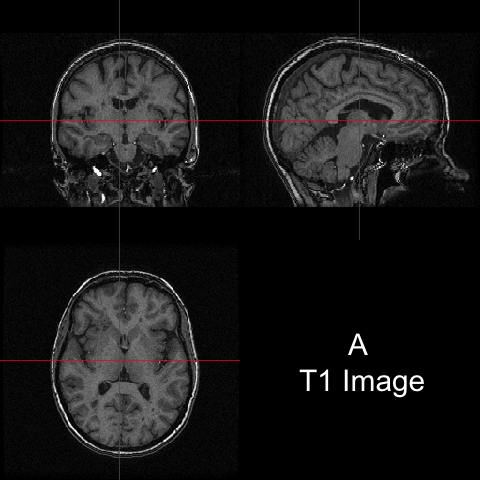
\includegraphics[width = 0.245\textwidth]{figure/T1_Ortho.png}
} \hspace*{-0.9em}
\hfill
  \subfloat{
  \label{bc_t1_ortho}
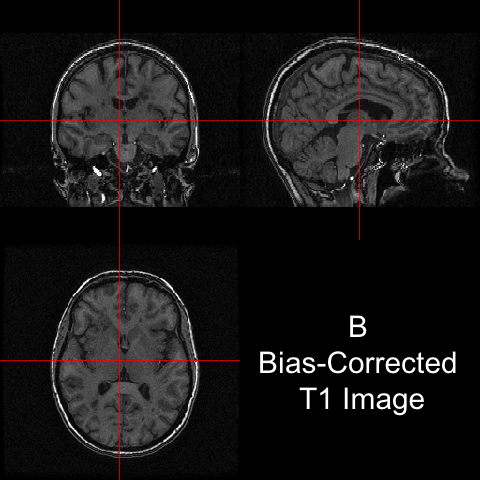
\includegraphics[width = 0.245\textwidth]{figure/BC_T1_Ortho.png} 
} \hspace*{-0.9em}
\hfill
  \subfloat{
  \label{t1_vs_bc_t1}
  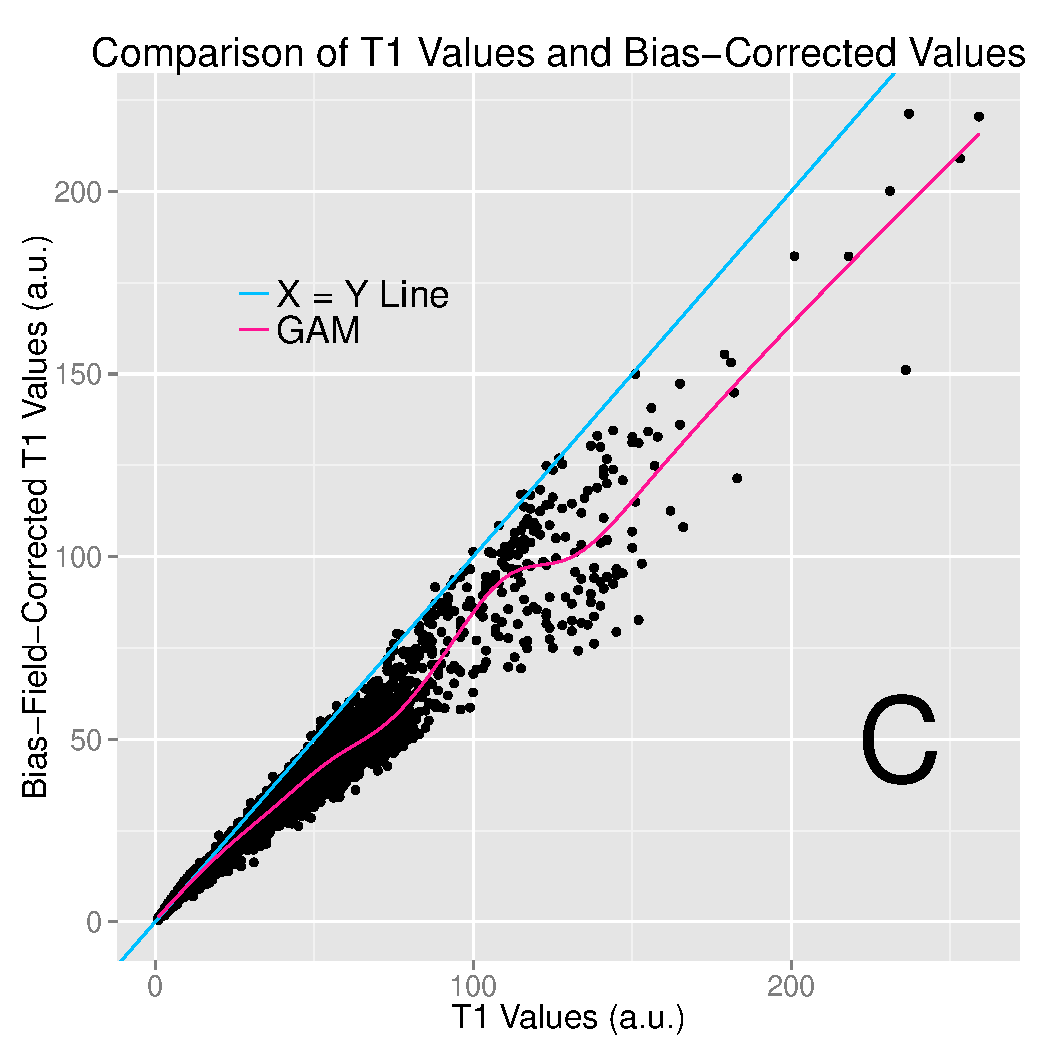
\includegraphics[width = 0.245\textwidth]{figure/plot_bc_data.pdf}
} \hspace*{-0.9em}
\hfill
  \subfloat{
  \label{t1_vs_bc_t1_zoom}
  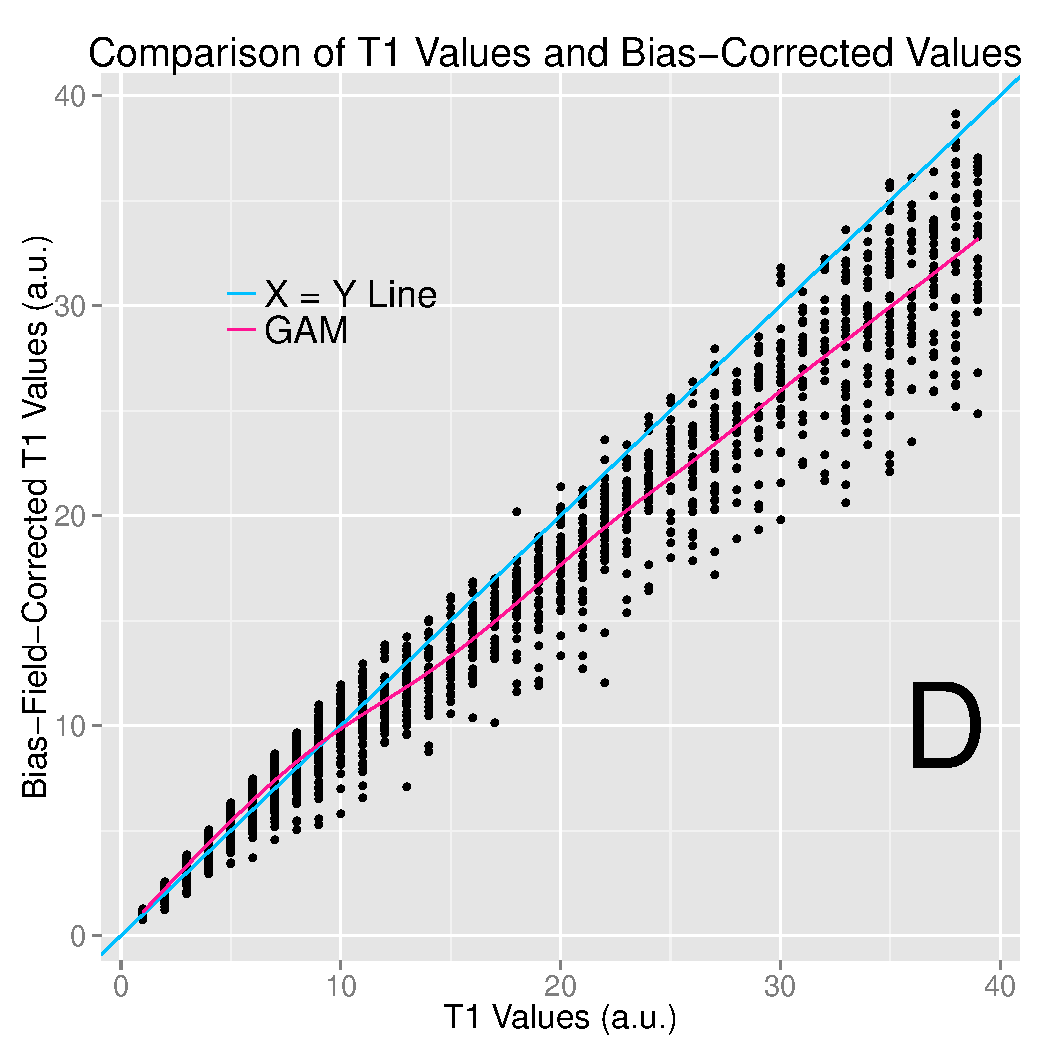
\includegraphics[width = 0.245\textwidth]{figure/plot_bc_data_zoom-1.pdf}
}
\caption[\bf Results of Inhomogeneity Correction.]{{\bf Results of Inhomogeneity Correction.}  We present the original T1 image~\protect\subref{t1_ortho}, bias-corrected T1 image~\protect\subref{bc_t1_ortho}, and the scatterplot of the sampled values comparing the values from the T1 image to the bias-corrected values \protect\subref{t1_vs_bc_t1}.  We see in panel~\protect\subref*{t1_vs_bc_t1} for values in the low range of the data ($< 10$), the T1 values and bias-corrected T1 values, on average, fall along the diagonal (blue line), which is further illustrated in panel~\protect\subref*{t1_vs_bc_t1_zoom}, which plots values $< 40$.  Values $> 10$ for the original T1 image are lower than the bias-corrected T1 values shown by a generalized additive model (GAM) smoother (pink line, panel~\protect\subref*{t1_vs_bc_t1}).  }
\label{fig:bias_correct}
\end{figure}

% Below we subset data where the T1 is not zero, as zero is the background voxel intensity and then subsample the data for visualization.  We also plot the data using \CRANpkg{ggplot2} \citep{wickham_ggplot2:_2009}, shown in figure~\ref{fig:bias_correct}\protect\subref*{t1_vs_bc_t1}.  Note, the scales are in arbitrary units (a.u.).



The blue line in Figure~\ref{fig:bias_correct}\protect\subref*{t1_vs_bc_t1} represents the 45$^{\circ}$ diagonal line, where the original and bias-corrected image intensities are equal ($X = Y$), and the pink line represents a generalized additive model (GAM) \citep{hastie_generalized_1990} scatterplot smoother estimate obtained using the \CRANpkg{mgcv} package \citep{wood_fast_2011}.  We see that for values in the low range of the data ($< 10$), the T1 values and bias-corrected T1 values, on average, fall along the diagonal, but in the higher range the bias-corrected values are lower.






\section{Within-visit co-registration}
All subsequent steps will be performed on the bias-corrected images.  We will first co-register the images within each separate visit to the T1 image from that visit.  This operation overlays the images on one another and allows us to investigate joint distributions of voxel intensities from different image modalities.  This is performed using FMRIB's Linear Image Registration Tool (FLIRT) \citep{jenkinson_global_2001, jenkinson_improved_2002}.  As the images are from the same individual, we may assume that the overall shape of the brain has not changed, but each scan may have undergone a translation and/or rotation in space.  Therefore, we will use a rigid-body transformation, with $6$ degrees of freedom (dof).  

%We will use another \code{data.frame} with image input and output names, including the T1 image of that visit, the image to be registered, the output transformation matrix and output filename.






The \pkg{fslr} command \code{flirt} calls the FSL command \code{flirt}, taking the input image (\code{infile}) and the reference image that serves as a template (\code{reffile}).  Any additional options for FLIRT can be passed using the \code{opts} argument.  We will use the defaults (i.e. trilinear interpolation) and the \code{-v} option for diagnostic messages to be printed.  Since we are doing a rigid-body transformation, we set the degrees of freedom (\code{dof}) to 6. Here we present the code for registering the baseline T2 image to the baseline T1 image; we will subsequently repeat this process for the baseline FLAIR and PD images and for the follow-up scans. 
\begin{Schunk}
\begin{Sinput}
flirt(reffile = "01-Baseline_T1_FSL_BiasCorrect",  
      infile = "01-Baseline_T2_FSL_BiasCorrect", 
      omat = "01-Baseline_T2_FSL_BiasCorrect_rigid_to_T1.mat", 
      dof = 6, 
      outfile = "01-Baseline_T2_FSL_BiasCorrect_rigid_to_T1", 
      opts = "-v")
\end{Sinput}
\end{Schunk}



The resulting image transformation is stored using the file name passed to the \code{omat} ({\bf o}utput {\bf mat}rix) argument.  This matrix can be used to transform other images, that were in the same space as the input image, to the reference image space.  The \pkg{fslr} package will currently only return \code{nifti} objects, and not a list of objects, such as the output image, transformation matrix, etc.  Thus, any transformation files that are needed after the command is executed must be specified.  

After co-registration, one could compare images of different modalities at the same voxels, such as T1 versus FLAIR images, which is presented in Figure~\ref{fig:coreg}.  The images are presented at the same cross section for the baseline T1 (Panel~\ref{ft1_ortho}) and FLAIR (Panel~\ref{flair_t1_ortho}) images.  The same brain areas are presented in each modality, indicating adequate registration.  
% The scatterplot illustrates the joint distribution of intensities for these images; the per-voxel signal generated by each imaging modality are in arbitrary units and should not necessarily be equal or follow a particular (e.g.~linear) relationship.


In the previous example, we presented a rigid-body transformation, using the default parameters.  \code{flirt} has options for different cost functions to optimize over, interpolation operators to estimate voxel intensity, and additional degrees of freedom for performing affine transformations.  These options can be passed to the FSL \code{flirt} command using the \code{opts} argument in the \pkg{fslr} \code{flirt} function.  

Note that each \pkg{fslr} function has a corresponding help function, which is the \pkg{fslr} command appended with \code{.help()}, which prints out the FSL help page for that function.  For example, users can see which options can be changed in the FSL \code{flirt} command by executing the \code{flirt.help()} function.   Additional non-linear registration techniques are presented in the section~``Registration to the MNI Template''.  









\begin{figure}
  \subfloat{
  \label{ft1_ortho}
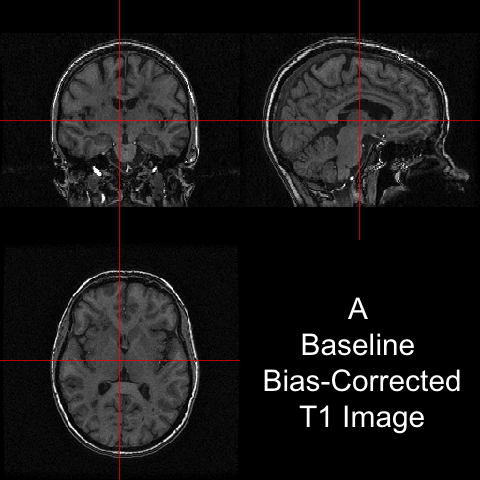
\includegraphics[width = 0.42\textwidth]{figure/BC_T1_Ortho_A.png}
}
\hfill
  \subfloat{
  \label{flair_t1_ortho}
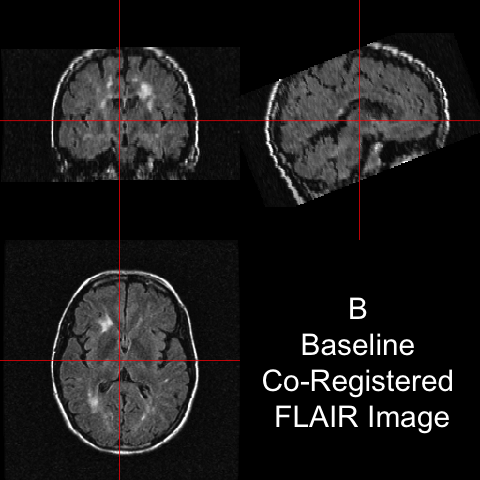
\includegraphics[width = 0.42\textwidth]{figure/FLAIR_Ortho_B_FLIRT.png} 
}
\caption[{\bf Results of within-visit co-registration.}]{{\bf Results of within-visit co-registration.}  We present the bias-corrected T1 image~\protect\subref{ft1_ortho} and the co-registered bias-corrected FLAIR image~\protect\subref{flair_t1_ortho}.  }
\label{fig:coreg}
\end{figure}


\section{Between-visit co-registration}
Though across-modality comparisons can be achieved by performing within-visit co-registration, across-visit registration is required for assessing within-modality differences between longitudinal scans.   To compute difference images, we co-register follow-up images to the baseline images within each modality.  Similar to the within-visit co-registration, we use a rigid-body transformation.  We will register the T1 images from baseline and follow-up, and apply this transformation to the co-registered-to-T1 images from above (see Figure~\ref{fig:reg} for illustration).  

\begin{figure}
\centering
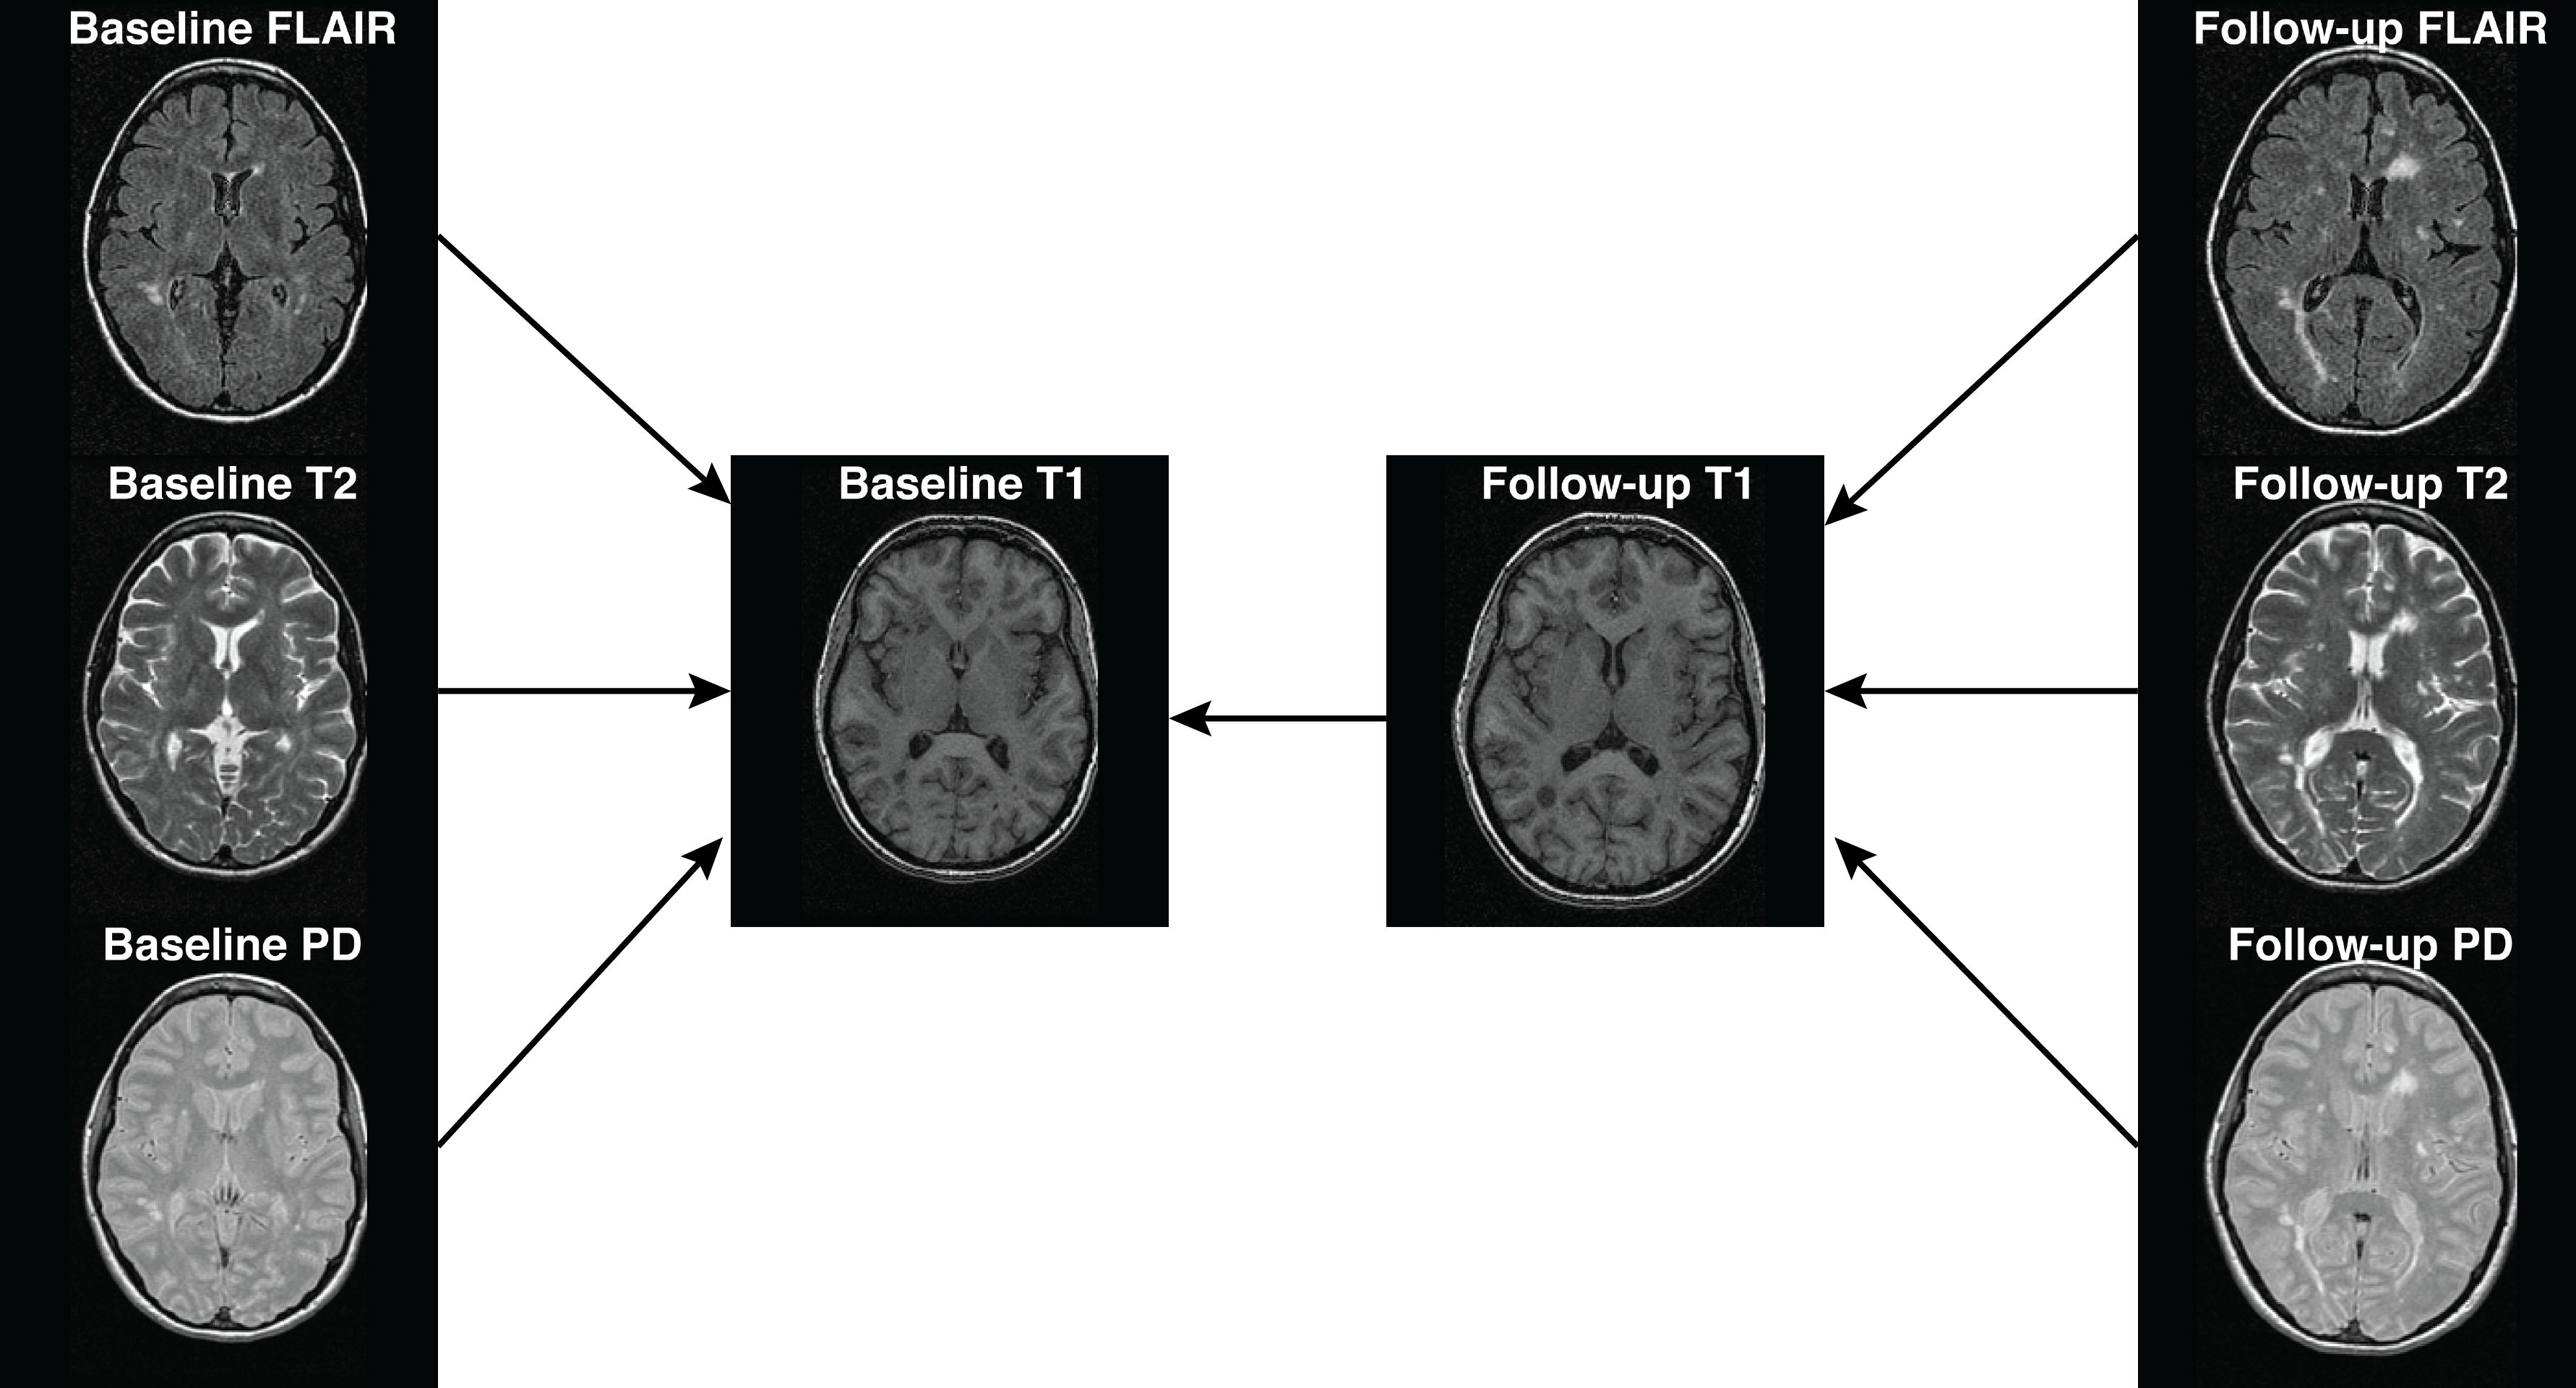
\includegraphics[width = 0.9\textwidth]{Reg_Figure_Option1.png}
\caption[{\bf Between-visit registration process.}]{{\bf Between-visit registration process.}  First, we registered all scans within a visit (baseline or follow-up) to the T1 image.  We then registered the follow-up T1 image to the baseline T1 image and applied the transformation to the follow-up T2, FLAIR, and PD images previously co-registered to the follow-up T1 image. }
\label{fig:reg}
\end{figure}

Though this registration involves two interpolations of the data and may not be optimal for within-modality comparisons, we have already obtained the co-registered-to-T1 images in the section ``Within-Visit Co-registration'' and must perform only one additional registration.  This operation also demonstrates how to apply transformation matrices in \pkg{fslr}.  Here we register the follow-up T1 image to the baseline T1 image, again using a rigid-body transformation (6 dof):

\gobblepars
\begin{Schunk}
\begin{Sinput}
flirt(reffile = "01-Baseline_T1_FSL_BiasCorrect", 
      infile = "01-Followup_T1_FSL_BiasCorrect", 
      omat = "01-Followup_T1_FSL_BiasCorrect_rigid_to_BaseT1.mat", 
      dof = 6,
      outfile = "01-Followup_T1_FSL_BiasCorrect_rigid_to_BaseT1", 
      opts = "-v")
\end{Sinput}
\end{Schunk}
\gobblepars


Now, both T1 images are aligned in the space of the baseline T1 image.  We present the results in Figure~\ref{fig:flirt}: the bias-corrected baseline T1 image in~\protect\subref*{flirt_base} and the co-registered bias-corrected follow-up T1 in~\protect\subref*{flirt_fup}.   The images displayed at the same cross section correspond to the same brain area, indicating a good registration.




\begin{figure}
  \subfloat{
  \label{flirt_base}
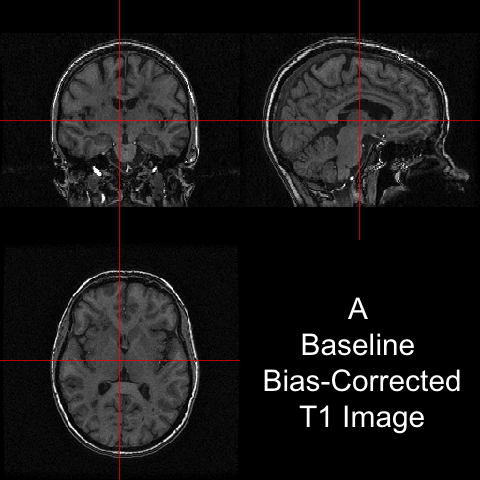
\includegraphics[width = 0.48\textwidth]{figure/BC_T1_Ortho_A.png}
}
\hfill
  \subfloat{
  \label{flirt_fup}
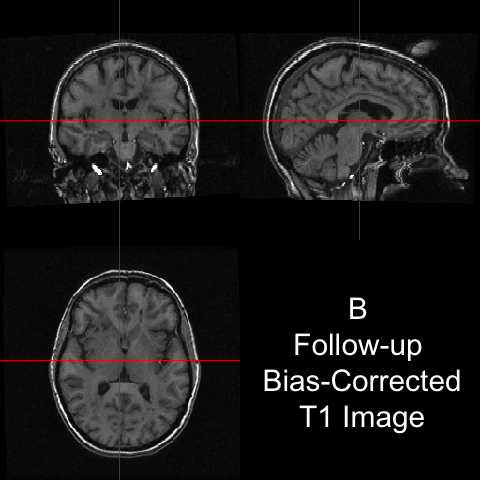
\includegraphics[width = 0.48\textwidth]{figure/FLIRT_Followup_T1.png} 
}
\caption[{\bf Results from FLIRT.}]{{\bf Results from FLIRT.} The bias-corrected baseline T1 is presented in~\protect\subref{flirt_base} and the registered bias-corrected follow-up T1 is presented in~\protect\subref{flirt_fup}, each displayed at the same intersection. We observe that the observed images correspond to the same brain area, indicating a good registration. }
\label{fig:flirt}
\end{figure}


Using the \code{flirt\_apply} function from \pkg{fslr}, we can apply the transformation matrix to the T2, PD, and FLAIR images from the follow-up visit, previously co-registered to the T1 from follow-up, to align them to the baseline T1 image space.  The code below aligns the follow-up T2 image, previously registered to the follow-up T1 image, to the baseline T1 image:

\newpage	
\begin{Schunk}
\begin{Sinput}
flirt_apply(reffile = "01-Baseline_T1_FSL_BiasCorrect", 
		# register to this
            infile = "01-Followup_T2_FSL_BiasCorrect_rigid_to_T1", 
            	# reg to Followup T1
            initmat = "01-Followup_T1_FSL_BiasCorrect_rigid_to_BaseT1.mat", 
            	#transform
            outfile = "01-Followup_T2_FSL_BiasCorrect_rigid_to_BaseT1" 
            	# output file
            ) 
\end{Sinput}
\end{Schunk}



In Figure~\ref{fig:reg_results}, we display each image after FLIRT has been applied.  Each image is in the baseline T1 image space, displayed at the same cross section.  Each panel shows the same brain areas across modalities, indicating adequate registration.  We see that some areas of the brain are cropped from the field of view, which may be problematic if relevant brain areas are removed.  We have registered all images with the skull and extracranial tissue included.  A better method may be to perform registration on brain tissues only, in which case we must perform brain extraction.

\begin{figure}
  \subfloat{
  \label{reg_t1_ortho}
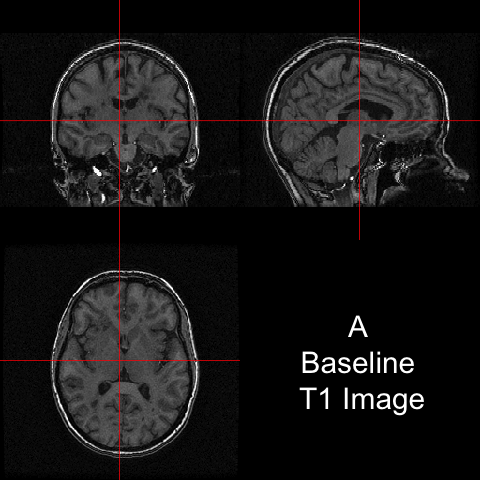
\includegraphics[width = 0.245\textwidth]{figure/BC_T1_Ortho_A_FLIRT.png}
} \hspace*{-0.9em}
\hfill
  \subfloat{
  \label{reg_t2_ortho}
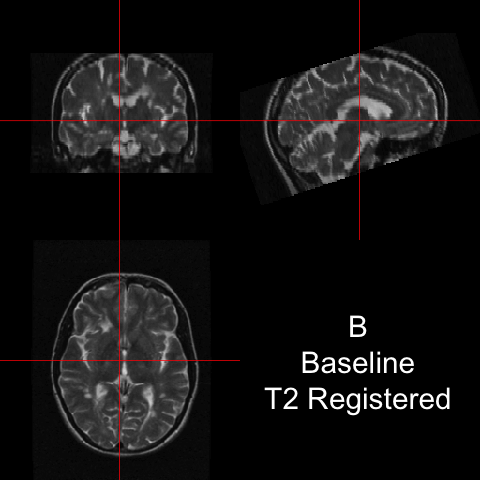
\includegraphics[width = 0.245\textwidth]{figure/01-Baseline_T2_FSL_BiasCorrect_rigid_to_T1.png} 
} \hspace*{-0.9em}
\hfill
  \subfloat{
  \label{reg_flair_ortho}
  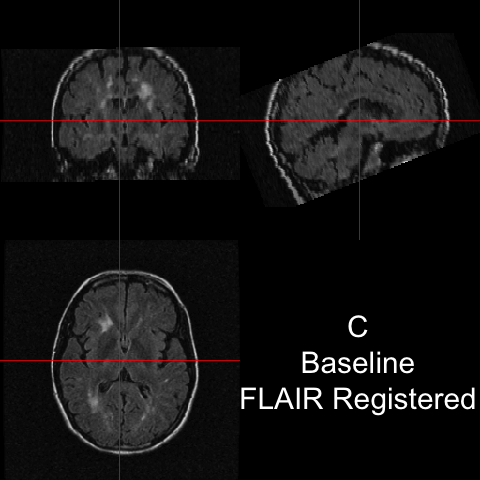
\includegraphics[width = 0.245\textwidth]{figure/01-Baseline_FLAIR_FSL_BiasCorrect_rigid_to_T1.png}
} \hspace*{-0.9em}
\hfill
  \subfloat{
  \label{reg_pd_ortho}
  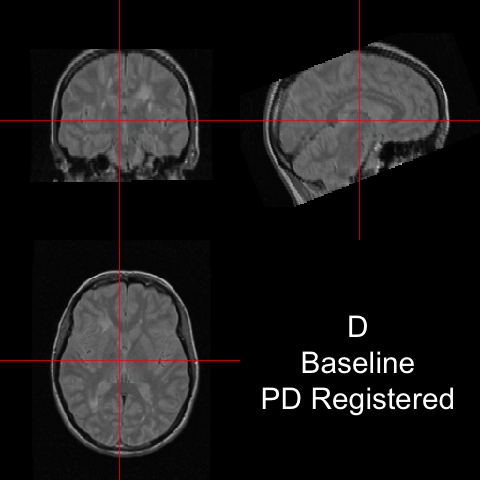
\includegraphics[width = 0.245\textwidth]{figure/01-Baseline_PD_FSL_BiasCorrect_rigid_to_T1.png}
} \hspace*{-0.9em}
\newline
  \subfloat{
  \label{reg_t1_ortho_fup}
  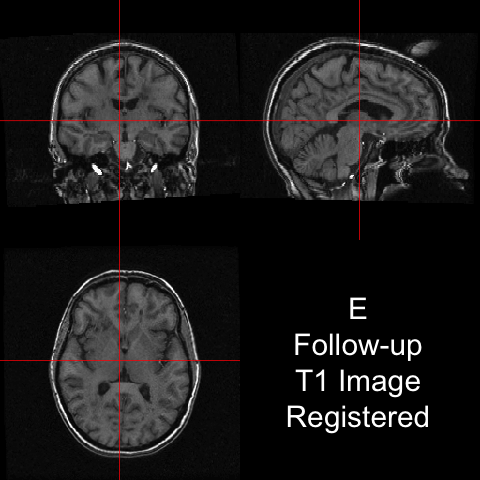
\includegraphics[width = 0.245\textwidth]{figure/E_FLIRT_Followup_T1.png} 
} \hspace*{-0.9em}
\hfill
  \subfloat{
  \label{reg_t2_ortho_fup}
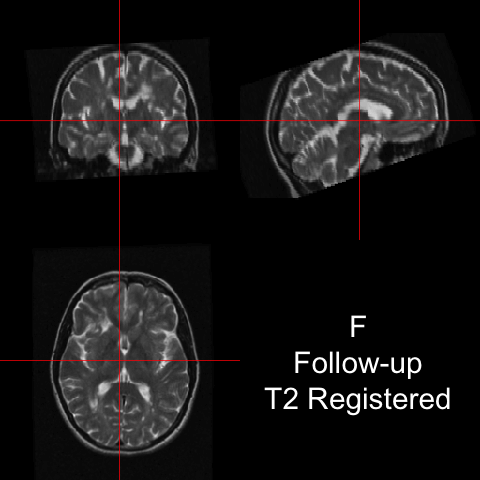
\includegraphics[width = 0.245\textwidth]{figure/01-Followup_T2_FSL_BiasCorrect_rigid_to_BaseT1.png} 
} \hspace*{-0.9em}
\hfill
  \subfloat{
  \label{reg_flair_ortho_fup}
  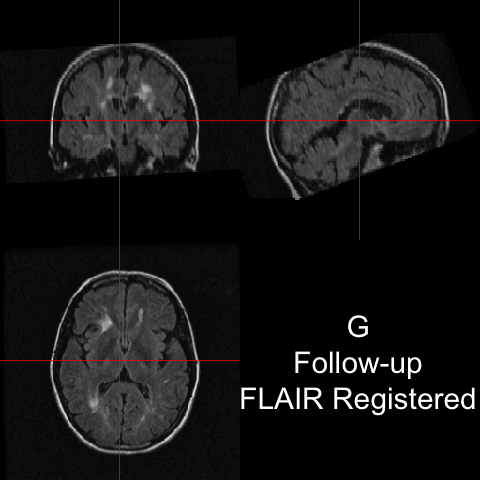
\includegraphics[width = 0.245\textwidth]{figure/01-Followup_FLAIR_FSL_BiasCorrect_rigid_to_BaseT1.png} 
} \hspace*{-0.9em}
\hfill
  \subfloat{
  \label{reg_pd_ortho_fup}
  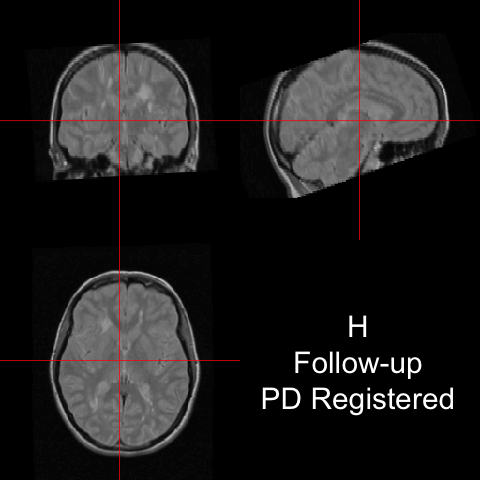
\includegraphics[width = 0.245\textwidth]{figure/01-Followup_PD_FSL_BiasCorrect_rigid_to_BaseT1.png} 
} \hspace*{-0.9em}
\caption[{\bf Between-visit registration results.}]{{\bf Between-visit registration results.} The complete set of acquired images, first co-registered within visit to the T1 image of that visit, then registered to the baseline T1 image using the follow-up T1 to baseline T1 transformation matrix.  All registrations performed rigid-body transformations.}
\label{fig:reg_results}
\end{figure}



\section{Brain extraction}
The process of extracting brain tissue from the acquired image, referred to as brain extraction or skull stripping, is a crucial step in many analyses.  We will perform brain extraction using FSL's brain extraction tool (BET) \citep{smith_fast_2002, jenkinson_bet2:_2005} using parameters recommended by \citet{popescu_optimizing_2012}, which were derived from patients with MS.  No other published R package on CRAN (e.g~ \CRANpkg{AnalyzeFMRI}, \CRANpkg{RNiftyReg}, or \CRANpkg{fmri}) has brain extraction functionality for brain imaging.  Other neuroimaging software provide brain extraction, such as AFNI \citep{cox_afni:_1996}, SPM \citep{ashburner_unified_2005}, and Freesurfer \citep{fischl_freesurfer_2012}, and multi-atlas label fusion techniques \citep{doshi_multi-atlas_2013}.
 


\begin{Schunk}
\begin{Sinput}
fslbet(infile =  '01-Baseline_T1', 
       outfile = "01-Baseline_T1_FSL_BiasCorrect_Brain", 
       opts = "-B -f 0.1 -v",  # from Popescu et al.
       betcmd = "bet", 
       intern=FALSE)
\end{Sinput}
\end{Schunk}


We ran BET on the non-corrected T1 image as the \code{-B} option performs inhomogeneity correction from FAST as part of the procedure.  The option \code{-f 0.1} denotes the fractional intensity (FI) parameter in BET: it varies between $0$ and $1$ and determines the location of the edge of the segmented brain image; smaller values correspond to larger brain masks. In Figure~\ref{fig:bet}, the bias-corrected T1 image is shown with the brain mask overlaid in red (panel~\protect\subref*{bet_mask}) and the resulting masked brain (panel~\protect\subref*{bet_brain}).  We see that the brain extraction performed well, not including any areas of the skull or the neck while not discarding brain tissue.  Towards the back of the brain, some areas of the subarachnoid space remain, which may be unacceptable for certain analyses, such as estimation of the volume of brain tissue.



\begin{figure}
  \subfloat{
  \label{bet_mask}
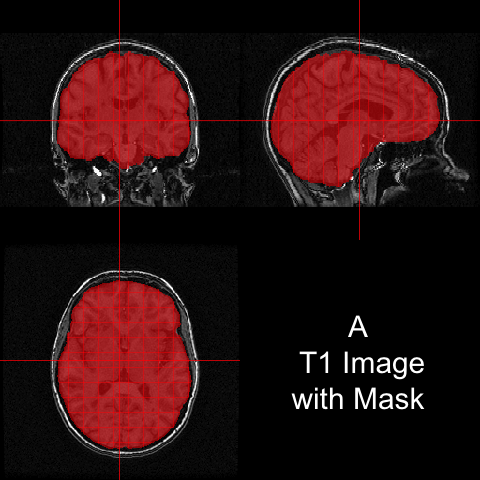
\includegraphics[width = 0.48\textwidth]{figure/plot_bet_mask.png}
}
\hfill
  \subfloat{
  \label{bet_brain}
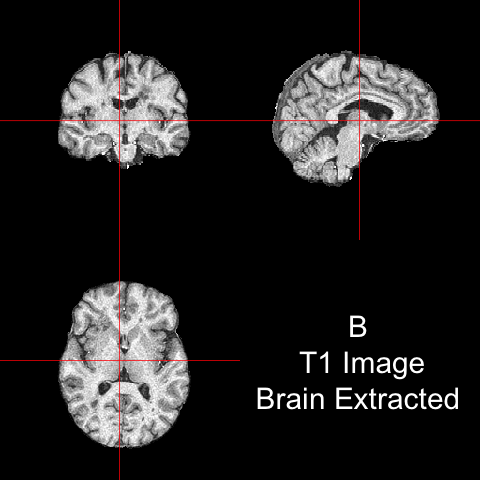
\includegraphics[width = 0.48\textwidth]{figure/plot_bet_brain.png} 
}
\caption[{\bf Results from BET.}]{{\bf Results from BET.} In~\protect\subref{bet_mask}, we show the bias-corrected T1 image with the mask from BET overlaid in red.  In~\protect\subref{bet_brain}, we display the extracted brain.  We see that the brain extraction performed well, not including any areas of the skull or the neck while not discarding large areas of the brain.}
\label{fig:bet}
\end{figure}

Note that \code{fslbet} writes both a file containing the brain-extracted image and another image containing the binary brain mask.  As all other images are registered to the baseline T1 space, we can use this mask to extract the brain from other images, such as the baseline T2 image, using the \pkg{fslr} function \code{fslmask}.  In this example, we mask the registered-to-T1, bias-corrected T2 image with the binary brain mask, save the image to the filename specified in \code{outfile}, and also set the \code{retimg} option to \code{TRUE}, indicating the \code{fslmask} command to {\bf ret}urn the {\bf im}a\textbf{g}e.  The returned object is a \code{nifti} object, assigned to the R object \code{mask}:
\begin{Schunk}
\begin{Sinput}
mask <- fslmask(file="01-Baseline_T2_FSL_BiasCorrect_rigid_to_T1", 
                mask = "01-Baseline_T1_FSL_BiasCorrect_Brain_mask",
                outfile = "01-Baseline_T2_FSL_BiasCorrect_rigid_to_T1_Brain", 
                retimg = TRUE)
\end{Sinput}
\end{Schunk}
\gobblepars


We now have all images in the same stereotaxic space with the brain extracted.  

\section{Registration to the MNI template}
In many studies, information is aggregated across a population of images from different participants.  For the information to have the same interpretation spatially across participants, images from all participants need to be aligned in the same stereotaxic space (``template'' space), requiring registration to a standard template image.  A frequently used set of templates are provided by MNI (Montreal Neurological Institute). We have registered the baseline T1 image to the MNI T1 template \citep{hutchison_symmetric_2006}, included with FSL.  As an individual's brain does not necessarily have the same size as the template, it is not appropriate to use rigid-body transformations.  Instead, non-linear transformations are needed.  As these are patients with MS and have lesions, different non-linear registrations to template space can have a large impact on the outcome of analysis (see \citet{eloyan_health_2014} for discussion).


We will first register the baseline T1 image to the T1 template using an affine registration, which can perform scaling and shearing operations in addition to translation and rotation.  Although an affine transformation has more degrees of freedom than a rigid transformation, it may not provide a registration sufficient for analysis.  We will then use FNIRT (FMRIB's Nonlinear Image Registration Tool) to achieve better overlap of local brain structures \citep{jenkinson_fsl_2012, andersson_non-linear_2007}.  As we are concerned with good overlap only in brain structures, and not in areas such as the skull, we will register the brain-extracted brain images to the brain-only template.  The \pkg{fslr} function \code{fnirt\_with\_affine} will register using \code{flirt} with an affine transformation and then non-linearly register this image to the template using \code{fnirt}.  If this affine transformation is not executed before \code{fnirt}, the image will not achieve the necessary scaling into the template space.


\gobblepars
\begin{Schunk}
\begin{Sinput}
fnirt_with_affine(infile = "01-Baseline_T1_FSL_BiasCorrect_Brain",
                  reffile = file.path(fsldir(), "data", 
                  "standard", "MNI152_T1_1mm_brain"),                     
                  flirt.omat = 
                  	"01-Baseline_T1_FSL_BiasCorrect_Brain_affine_toMNI.mat", 
                  flirt.outfile = 
                  	"01-Baseline_T1_FSL_BiasCorrect_Brain_affine_toMNI", 
                  outfile = "01-Baseline_T1_FSL_BiasCorrect_Brain_toMNI")
\end{Sinput}
\end{Schunk}
\gobblepars

\gobblepars

 
The results of the registration can be seen in Figure~\ref{fig:fnirt_slice}.  Each panel represents a different axial slice ($z =$ 25, 45, 92, or 137) in the template space of the template image (\protect\subref*{mni_ortho_25}, \protect\subref*{mni_ortho_45}, \protect\subref*{mni_ortho_92}, \protect\subref*{mni_ortho_137}) or the registered T1 image (\protect\subref*{t1_warp_25}, \protect\subref*{t1_warp_45}, \protect\subref*{t1_warp_92}, \protect\subref*{t1_warp_137}).  Each slice shows the registered T1 image has similar brain structure represented in the same area as the template image, indicating good registration.


% \begin{figure}
%   \subfloat{
%   \label{mni_ortho}
% 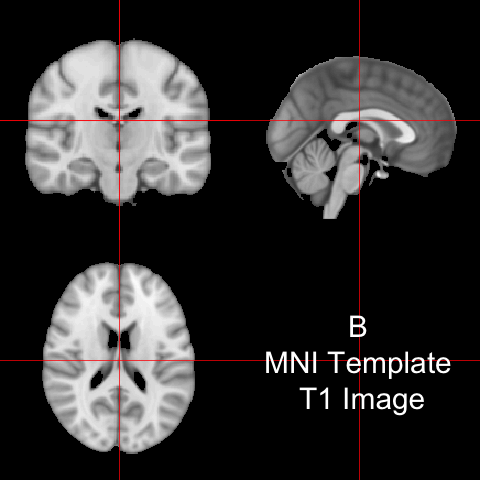
\includegraphics[width = 0.48\textwidth]{figure/MNI_Ortho.png} 
% }
% \hfill
%   \subfloat{
%   \label{t1_warp}
% 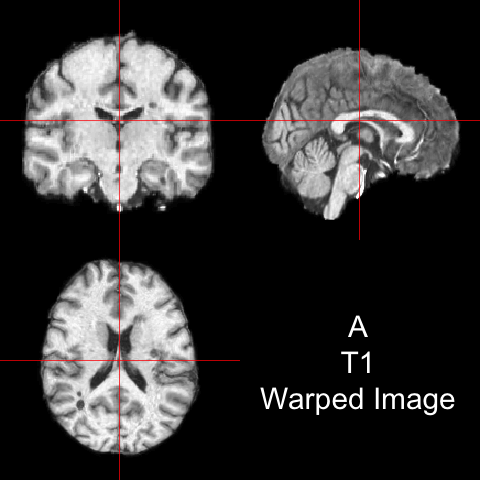
\includegraphics[width = 0.48\textwidth]{figure/T1_MNI_Warp.png}
% }
% \caption{{\bf Results from FNIRT.} In~\protect\subref{mni_ortho}, we display the MNI template image.  In~\protect\subref{t1_warp} we display the registered-to-template, brain-extracted T1 image.  We note that areas of the brain coincide between the template and registered image.}
% \label{fig:fnirt_ortho}
% \end{figure}


\begin{figure}
  \subfloat{
  \label{mni_ortho_25}
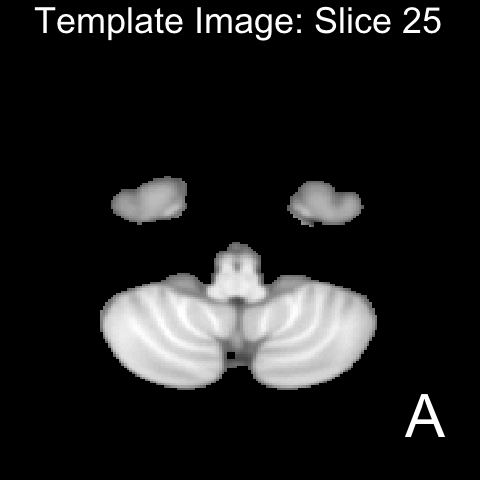
\includegraphics[width = 0.245\textwidth]{figure/MNI_Warp_Slice_25.png} 
} \hspace*{-0.9em}
  \subfloat{
  \label{t1_warp_25}
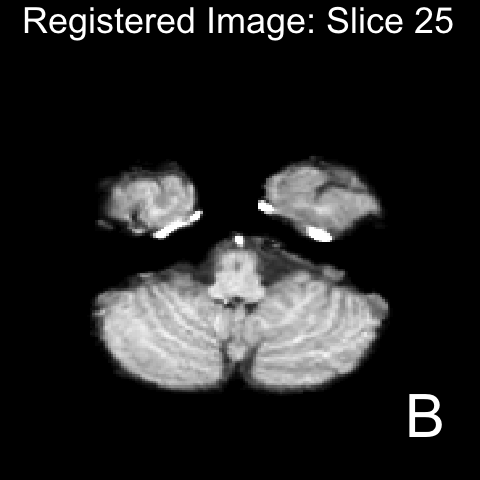
\includegraphics[width = 0.245\textwidth]{figure/T1_MNI_Ortho_Slice_25.png}
} \hspace*{-0.9em}
  \subfloat{
  \label{mni_ortho_45}
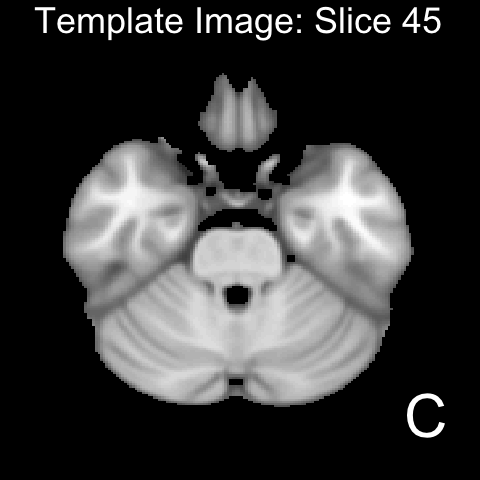
\includegraphics[width = 0.245\textwidth]{figure/MNI_Warp_Slice_45.png} 
} \hspace*{-0.9em}
  \subfloat{
  \label{t1_warp_45}
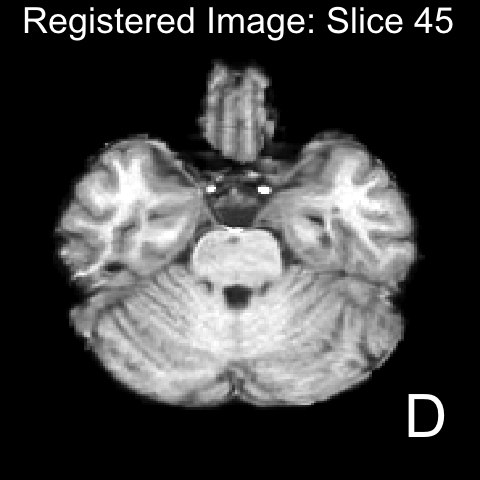
\includegraphics[width = 0.245\textwidth]{figure/T1_MNI_Ortho_Slice_45.png}
}\hspace*{-0.9em}
\newline
  \subfloat{
  \label{mni_ortho_92}
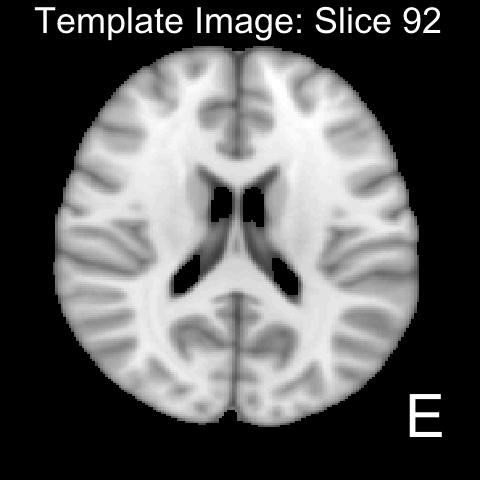
\includegraphics[width = 0.245\textwidth]{figure/MNI_Warp_Slice_92.png} 
} \hspace*{-0.9em}
  \subfloat{
  \label{t1_warp_92}
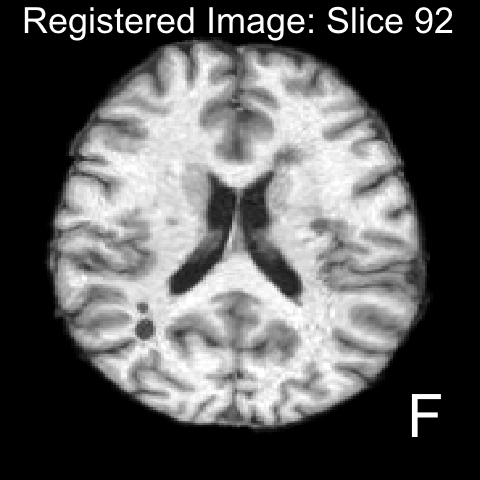
\includegraphics[width = 0.245\textwidth]{figure/T1_MNI_Ortho_Slice_92.png}
} \hspace*{-0.9em}
  \subfloat{
  \label{mni_ortho_137}
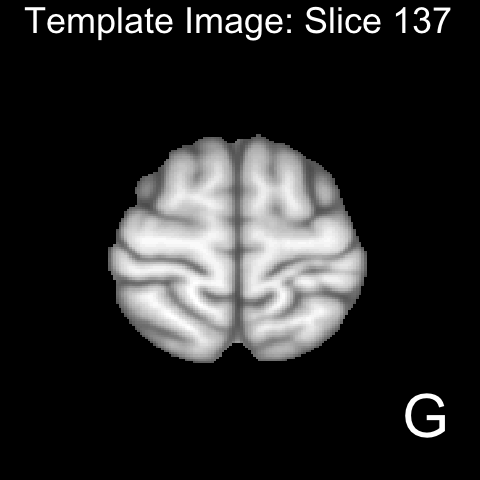
\includegraphics[width = 0.245\textwidth]{figure/MNI_Warp_Slice_137.png} 
} \hspace*{-0.9em}
  \subfloat{
  \label{t1_warp_137}
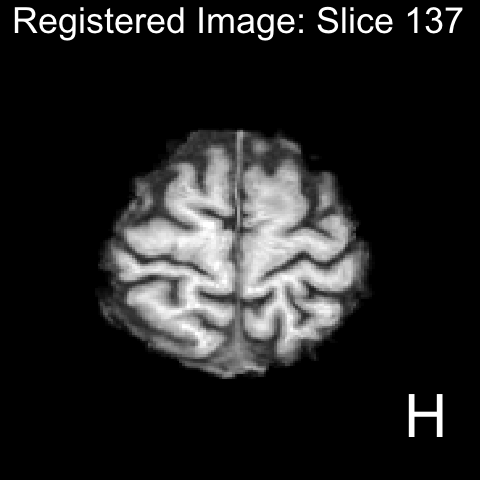
\includegraphics[width = 0.245\textwidth]{figure/T1_MNI_Ortho_Slice_137.png}
}\hspace*{-0.9em}
\caption[{\bf Results from FNIRT.}]{{\bf Results from FNIRT.} We present different axial slices of the template (\protect\subref*{mni_ortho_25}, \protect\subref*{mni_ortho_45}, \protect\subref*{mni_ortho_92}, \protect\subref*{mni_ortho_137}) and the registered T1 image (\protect\subref*{t1_warp_25}, \protect\subref*{t1_warp_45}, \protect\subref*{t1_warp_92}, \protect\subref*{t1_warp_137}).  The slices represented are 25 (\protect\subref*{mni_ortho_25}, \protect\subref*{t1_warp_25}), 45 (\protect\subref*{mni_ortho_45}, \protect\subref*{t1_warp_45}), 92 (\protect\subref*{mni_ortho_92}, \protect\subref*{t1_warp_92}) and 137 (\protect\subref*{mni_ortho_137}, \protect\subref*{t1_warp_137}).  We note that areas of the brain coincide between the template and registered image.}
\label{fig:fnirt_slice}
\end{figure}



\subsection{Applying transformations to co-registered data}
Since all the data is represented in the same image space, we can apply the estimated affine transformation and non-linear warping coefficient field to each image to represent that image in template space.  The affine transformation must be applied with \code{flirt\_apply} and the warping coefficient using \code{fsl\_applywarp}, which calls the FSL \code{applywarp} function.  



Here we present the application of the transformations to the baseline T2 image, previously registered to the baseline T1.  

\begin{Schunk}
\begin{Sinput}
flirt_apply(infile = "01-Baseline_T2_FSL_BiasCorrect_rigid_to_T1_Brain",
            reffile = file.path(fsldir(), "data", "standard", "MNI152_T1_1mm_brain"),
            initmat = "01-Baseline_T1_FSL_BiasCorrect_Brain_affine_toMNI.mat",
            outfile = "01-Baseline_T2_FSL_BiasCorrect_rigid_to_T1_Brain_toMNI")
fsl_applywarp(infile = "01-Baseline_T2_FSL_BiasCorrect_rigid_to_T1_Brain_toMNI",
              reffile = file.path(fsldir(), "data", "standard", "MNI152_T1_1mm_brain"),          
              warpfile = "01-Baseline_T1_FSL_BiasCorrect_Brain_affine_toMNI_warpcoef",
              outfile = "01-Baseline_T2_FSL_BiasCorrect_rigid_to_T1_Brain_toMNI")
\end{Sinput}
\end{Schunk}

These two operations can also be performed in a single call to the \pkg{fslr} \code{fnirt\_with\_affine\_apply} function.  

With multiple participants, this process yields a multi-person, multi-modal, longitudinal imaging dataset that can be used for analyses.





\section{Conclusion}
The neuroimaging community has developed a large collection of tools for image processing and analysis.  R has a number of packages to perform operations on images; \BIOpkg{EBImage} is one good example \citep{EBImage}. Much of the fundamental functionality of neuroimage processing is not currently available in R, such as brain extraction and tissue segmentation.  We present \pkg{fslr} to provide R users functions for image processing and analysis that are based on FSL, an established image processing and analysis software suite.  Interfacing R with existing, powerful software provides users with thoroughly-tested software and an additional community of users, which would not be available if the functions were rewritten in R.  \pkg{fslr} should be easy to use for any standard R user; the workflow allows R users to manipulate array-like \code{nifti} objects, pass them to \pkg{fslr} functions, which return \code{nifti} objects.  Moreover, as FSL and R are open source and free, this software is readily available to all users.  

There has been an increasing popularity of similar interfacing of tools within the Python community such as Nipype \citep{gorgolewski_nipype:_2011} (https://qa.debian.org/popcon.php?package=nipype).  As many users of R may not have experience with Python or bash scripting, we believe \pkg{fslr} provides a lower threshold for use in the R community.  Other packages provide R users additional neuroimaging processing functionality such as \CRANpkg{AnalyzeFMRI} \citep{bordier_temporal_2011}, \CRANpkg{RNiftyReg} \citep{modat_rniftyreg:_2013}, and \CRANpkg{fmri} \citep{tabelow_statistical_2011}.   

For example, other inhomogeneity correction methods exist, such as the popular N3 \citep{sled_nonparametric_1998} and N4 \citep{tustison_n4itk:_2010}, methods which are not implemented in \pkg{fslr}. \pkg{ANTsR} (\url{http://stnava.github.io/ANTsR/index.html}) is a currently unpublished R package that interfaces with the ANTs (advanced normalization tools) software suite \citep{avants_reproducible_2011}.  ANTs has implementations of these correction methods, an increased set of registration techniques, and other methods for image processing.  Other packages such as this, along with \pkg{fslr}, can create a diverse set of tools for neuroimaging within R, building on preexisting and widely-accepted software.  

%For example, we present one inhomogeneity correction method, yet other inhomogeneity correction methods exist, such as the popular N3 \citep{sled_nonparametric_1998} and novel N4 \citep{tustison_n4itk:_2010}, which are not implemented in \pkg{fslr}.  ANTsR (\url{http://stnava.github.io/ANTsR/index.html}), an R package that interfaces with the ANTs (advanced normalization tools) software suite \citep{avants_reproducible_2011}, has implementations of these correction methods and an increased set of registration techniques within R.

Most importantly, as \pkg{fslr} is based on the R framework, all the benefits of using R are available, such as dynamic documents, reproducible reports, customized figures, and state-of-the-art statistical methods.  These benefits provide unique functionality compared to other software packages for neuroimaging.  

All data and code processed here is located at \url{https://github.com/muschellij2/FSLR_Data}.  


%
%\section{Smoothing}
%In many analyses, integrating neighboring voxels intensities can increase information.  







% \begin{figure}
%   \subfloat{
%   \label{bet_img}
% 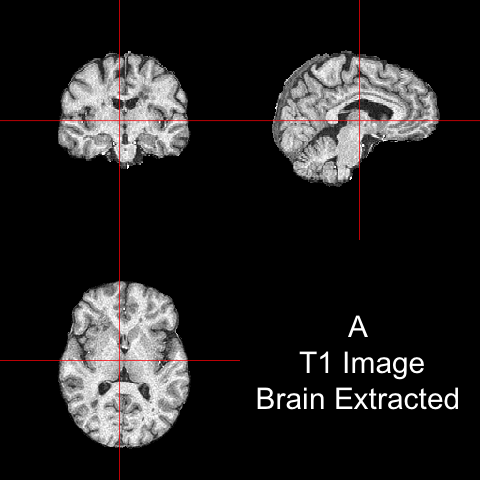
\includegraphics[width = 0.48\textwidth]{figure/Bet_Brain_A.png}
% }
% \hfill
%   \subfloat{
%   \label{bet_smooth}
% 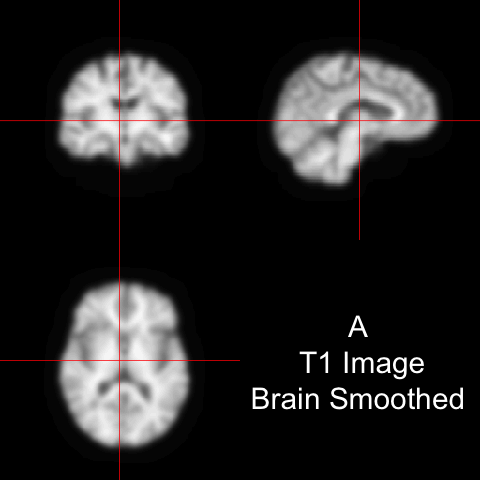
\includegraphics[width = 0.48\textwidth]{figure/T1_Smooth_Img.png}
% }
% \caption{{\bf Smoothing the Baseline T1 Brain Image.}  }
% \label{fig:smooth}
% \end{figure}


\section{Supplemental material}


\subsection{Smoothing images}
Let us show how to pass a Gaussian smoother over an image using \code{fslsmooth} (FSL \code{fslmaths -s} function).  First we will read in the registered-to-template baseline T1 brain image:

\gobblepars
\begin{Schunk}
\begin{Sinput}
t1_to_temp = readNIfTI("01-Baseline_T1_FSL_BiasCorrect_Brain_toMNI", reorient=FALSE)
\end{Sinput}
\end{Schunk}

We will smooth the image using a Gaussian smoother with $\sigma = 3\text{mm}^3$: 

\gobblepars
\begin{Schunk}
\begin{Sinput}
smooth = fslsmooth(t1_to_temp, sigma = 3, retimg=TRUE)
\end{Sinput}
\end{Schunk}

The result is presented in Figure~\ref{fig:fslr_func}\protect\subref*{smooth}.


\subsection{Thresholding images}
The \pkg{fslr} \code{fslbin} function will binarize a \code{nifti} image object: all values $\leq 0$ are set to $0$, and set to $1$ otherwise.  Let us binarize the registered image:


\gobblepars
\begin{Schunk}
\begin{Sinput}
binned = fslbin(t1_to_temp, retimg=TRUE)
\end{Sinput}
\end{Schunk}

The result is presented in Figure~\ref{fig:fslr_func}\protect\subref*{bin}.



The \pkg{fslr} \code{fslthresh} function provides more control for thresholding by setting a lower threshold (\code{thresh} argument) and upper threshold (\code{uthresh} argument).  These thresholds are inclusive, and will set values less than (but not equal to) \code{thresh} or greater than (but not equal to) \code{uthresh} to $0$.  Voxels with values between \code{thresh} and \code{uthresh} (inclusive) will be returned as their original value.  Let us threshold the smoothed image between $30$ and $50$:


\gobblepars
\begin{Schunk}
\begin{Sinput}
thresh = fslthresh(t1_to_temp, thresh = 30, uthresh = 50, retimg=TRUE)
\end{Sinput}
\end{Schunk}

The result is presented in Figure~\ref{fig:fslr_func}\protect\subref*{thresh}.

\subsection{Eroding and dilating images}
In many applications, one wants to erode (i.e. shrink) an image mask.  The \pkg{fslr} function \code{fslerode} performs this operations.  Note, if no options are specified for the kernel (in the \code{kopts} argument), the default $3\times3\times3$ voxel box kernel is used.  Here we erode the binarized image from above and plot the voxels eroded:




\begin{Schunk}
\begin{Sinput}
eroded = fslerode(binned, retimg=TRUE)
\end{Sinput}
\end{Schunk}

The result is presented in Figure~\ref{fig:fslr_func}\protect\subref*{ero}.  If one inverts the binary mask, performs erosion, and then inverts the resulting erosion mask, this procedure is equivalent to dilation.  The \pkg{fslr} function \code{fsldilate} (version 1.4 and above) will also perform image dilation.

\begin{figure}
  \subfloat{
  \label{smooth}
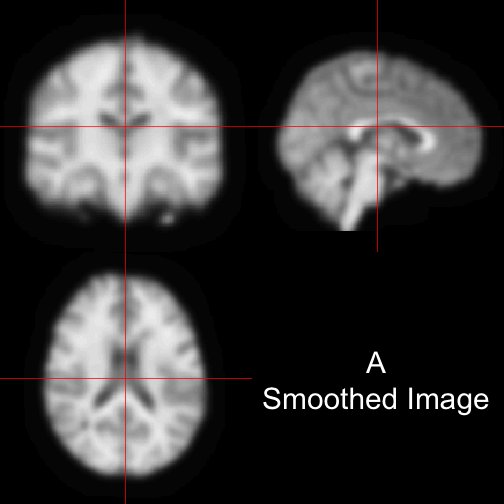
\includegraphics[width = 0.245\textwidth]{figure/smoother-1.png}
} \hspace*{-0.9em}
\hfill
  \subfloat{
  \label{bin}
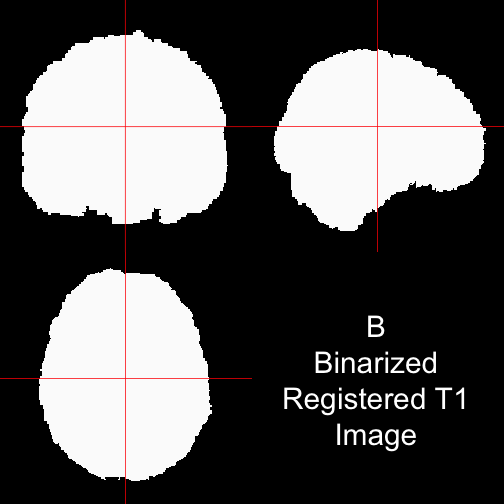
\includegraphics[width = 0.245\textwidth]{figure/binned-1.png}
} \hspace*{-0.9em}
\hfill
  \subfloat{
  \label{thresh}
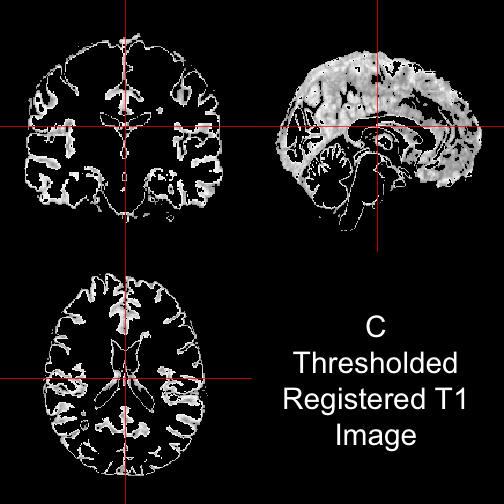
\includegraphics[width = 0.245\textwidth]{figure/thresh-1.png} 
} \hspace*{-0.9em}
\hfill
  \subfloat{
  \label{ero}
  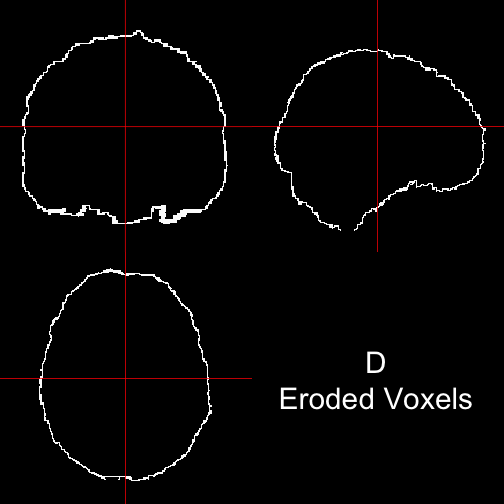
\includegraphics[width = 0.245\textwidth]{figure/ero-1.png}
}
\caption[{\bf Results of \pkg{fslr} functions.}]{{\bf Results of \pkg{fslr} functions.}  We present the smoothed registered-to-template T1 image~\protect\subref{smooth}, binarized image~\protect\subref{bin}, thresholded image~\protect\subref{thresh}, and image of the eroded voxels after eroding the binarized image \protect\subref{ero}.  }
\label{fig:fslr_func}
\end{figure}


\subsection{Extracting image information}
Although most \pkg{fslr} functions provide an image as the designated output, one may wish to extract image information from a NIfTI file on disk, without reading it into R.  The \pkg{fslr} \code{fslstats}, \code{fslval}, and \code{fslhd} functions are particularly useful and call functions of the same name from FSL.

For example, we can extract the number of slices in of the third dimension of the bias-corrected T1 image using \code{fslval}:
\begin{Schunk}
\begin{Sinput}
fslval("01-Baseline_T1_FSL_BiasCorrect_Brain", keyword = "dim3")
\end{Sinput}
\end{Schunk}
\gobblepars
\begin{Schunk}
\begin{Soutput}
[1] "124"
\end{Soutput}
\end{Schunk}

We could also extract the entire header using \code{fslhd} and assign it to an object:
\begin{Schunk}
\begin{Sinput}
img_hdr = fslhd("01-Baseline_T1_FSL_BiasCorrect_Brain")
\end{Sinput}
\end{Schunk}

We can extract the mean of the image of non-zero voxels:
\begin{Schunk}
\begin{Sinput}
fslstats("01-Baseline_T1_FSL_BiasCorrect_Brain", opts = "-M")
\end{Sinput}
\end{Schunk}
\gobblepars
\begin{Schunk}
\begin{Soutput}
[1] "51.264791"
\end{Soutput}
\end{Schunk}

Overall, there are many functions and options that allow the user to compute statistics or obtain header information from an image on disk without having to load it into R, which can reduce computation time.  

\subsection{Additional \pkg{fslr} functionality}

Although the main goal of \pkg{fslr} is to interface R and FSL, there is a set of functions in \pkg{fslr} that are not designed to interface with FSL, but rather provide helper functions for \code{nifti} objects from the \pkg{oro.nifti} package.  We will display 2 example functions: \code{cal\_img} and \code{niftiarr}.  The \code{cal\_img} function resets the \code{cal\_min} and \code{cal\_max} slots on a \code{nifti} object, which are used to determine colors when plotting.  The \code{niftiarr} function copies a \code{nifti} object and replaces the \code{.Data} slot, which contains the actual image intensity values, with a provided array. 

Let us illustrate by discussing 2 ways to mask an image.   We will read in the bias-corrected T1 image and the mask from BET:



\begin{Schunk}
\begin{Sinput}
base_t1 = readNIfTI("01-Baseline_T1_FSL_BiasCorrect", reorient=FALSE)
base_t1_mask = readNIfTI("01-Baseline_T1_FSL_BiasCorrect_Brain_mask", reorient=FALSE)
\end{Sinput}
\end{Schunk}


One way to mask the T1 image is to multiply the image by the binary mask:
\begin{Schunk}
\begin{Sinput}
base_t1_1 = base_t1 * base_t1_mask
class(base_t1_1)
\end{Sinput}
\begin{Soutput}
[1] "array"
\end{Soutput}
\end{Schunk}

We see that the resulting object is an array and not a \code{nifti} object (as of \pkg{oro.nifti} version \code{0.4.3}).  This may be a problem when trying to plot or manipulate this object using methods for \code{nifti} objects.  To address this problem, the \code{niftiarr} function in \pkg{fslr} inputs a \code{nifti} object and an \code{array}, and returns a \code{nifti} object with the provided \code{array} in the \code{.Data} slot, copying over the image information from the input \code{nifti} object.   As of \pkg{oro.nifti} version \code{0.5.0}, the output from above will be a \code{nifti} object, but the function explained below, \code{niftiarr}, is still of use in cases when creating a new \code{nifti} object.

\begin{Schunk}
\begin{Sinput}
base_t1_1 = niftiarr(base_t1, base_t1_1)
class(base_t1_1)
\end{Sinput}
\begin{Soutput}
[1] "nifti"
attr(,"package")
[1] "oro.nifti"
\end{Soutput}
\end{Schunk}

Another way of masking the image is to subset the values of the image that are not in the mask and setting those values to $0$ (or some other value).
\begin{Schunk}
\begin{Sinput}
base_t1_2 = base_t1
base_t1_2[base_t1_mask == 0] = 0
class(base_t1_2)
\end{Sinput}
\begin{Soutput}
[1] "nifti"
attr(,"package")
[1] "oro.nifti"
\end{Soutput}
\end{Schunk}

We see that this correctly returns an object of class \code{nifti}.  One problem is that the we have changed the data in the \code{nifti} object  \code{base\_t1\_2} but did not reset the other slots in this object to reflect this change.


In a \code{nifti} object, the \code{cal\_min} and \code{cal\_max} slots equal the minimum and maximum values, respectively, of the data.   The \code{orthographic} function (from \pkg{oro.nifti}) uses these values for plotting; also, if these slots do not equal the minimum and maximum, the \code{writeNIfTI} function (from \pkg{oro.nifti}) will fail.  The \code{cal\_img} is a simple helper function that will set the  \code{cal\_min} and \code{cal\_max} slots to the correct values.  Let us look at the range of the data and the \code{cal\_min} and \code{cal\_max} slots:
\begin{Schunk}
\begin{Sinput}
range(base_t1_2)
\end{Sinput}
\begin{Soutput}
[1]   0.0000 409.3908
\end{Soutput}
\begin{Sinput}
c(base_t1_2@cal_min, base_t1_2@cal_max)
\end{Sinput}
\begin{Soutput}
[1] 0 0
\end{Soutput}
\end{Schunk}
An issue with \code{readNIfTI} function from \pkg{oro.nifti} is that the \code{cal\_min} and \code{cal\_max} slots may be both read as zero.  Let us set these to the range using the \code{cal\_img} command from \pkg{fslr}:
\begin{Schunk}
\begin{Sinput}
base_t1_2 = cal_img(base_t1_2)
c(base_t1_2@cal_min, base_t1_2@cal_max)
\end{Sinput}
\begin{Soutput}
[1]   0.0000 409.3908
\end{Soutput}
\end{Schunk}
We see that after these operations are done 2 in different ways, the resulting \code{nifti} objects are equivalent.  
\begin{Schunk}
\begin{Sinput}
identical(base_t1_1, base_t1_2)
\end{Sinput}
\begin{Soutput}
[1] TRUE
\end{Soutput}
\end{Schunk}

Additional helper functions such as these are included in \pkg{fslr} for plotting and image manipulation.

%\section{Difference between Images}
%Now that we have the images in the same space and a mask for the brain image, we can take a difference of brain-only tissues.  



% \bibliography{FSLR}
%\bibliography{muschelli}
%\AtEveryBibitem{\clearfield{note}}    % clears notes

%
%\section{Supplemental Material}
%\section{Z-score and threshold}











\cleardoublepage
\printbibliography[title={References}]
\end{refsection}

\begin{refsection}[ich_chapter/ich_chapter.bib]
\chapter{PItcHPERFeCT: Primary Intracranial Hemorrhage Probability Estimation using Random Forests on CT}
\label{chap:ich_seg}


\renewcommand{\thesubfigure}{\Alph{subfigure}} % OK


\newcommand{\mywidth}{0.23}

\newcommand{\stubber}[1]{figures/Reseg_161-413_20110710_1619_CT_2_HEAD_Head#1.png}
%trim = 3in 10in 4in 3in, clip, 
\newcommand{\makeimg}[2]{\includegraphics[width=#1\linewidth]{\stubber{#2}}}











\section{Introduction}


%Bleeding may cause distension of the brain structures an increase in potentially lethal intracranial pressure (ICP).  ICH is a serious condition; it accounts for approximately 10-15\% of all strokes, corresponding to an estimated 79,500 annual cases \citep{go_heart_2013} and approximately 30,000 deaths \citep{qureshi_spontaneous_2001} in the US and approximately 5 million cases worldwide \citep{krishnamurthi_global_2014}. In addition to the increased likelihood of death, ICH has debilitating health effects on survivors who do not have full functional recovery after stroke.

Intracerebral hemorrhage (ICH) is a neurological condition that results from a blood vessel rupturing into the tissue and possibly the ventricles of the brain.   The use of X-ray computed tomography (CT) scans allows clinicians and researchers to qualitatively and quantitatively describe the characteristics of a hemorrhage to guide interventions and treatments.  CT scanning is widely available and is the most commonly used diagnostic tool in patients with ICH \citep{sahni_management_2007}.  The volume of ICH has been consistently demonstrated to be an important diagnostic predictor of stroke severity, long-term functional outcome, and mortality \citep{broderick_volume_1993, hemphill_ich_2001, tuhrim_volume_1999}.  ICH volume change is also common primary outcome \citep{anderson_intensive_2008, anderson_effects_2010, qureshi_association_2011, mayer_recombinant_2005} and secondary outcome \citep{morgan_preliminary_2008_mistie, anderson_intensive_2008, morgan_preliminary_2008_clear} in clinical trials.  Moreover, the location of the ICH has been shown to affect functional outcome in patients with stroke \citep{rost_prediction_2008, castellanos_predictors_2005}.

ICH volume can be rapidly measured using techniques such as the ABC/2 method \citep{broderick_volume_1993}.  In this method, a reader chooses which slice has the largest area of hemorrhage, draws a line along the longest axis of the hemorrhage (denoted A) and the orthogonal line that bisects the hemorrhage (B).  The reader then counts the number of slices where hemorrhage is present (C).  The volume estimate is $\frac{A\times B\times C}{2}$, which is an approximation of an ellipsoid \citep{kothari_abcs_1996}.  As this method only requires 3 measurements, this method can be done rapidly. 

Although ABC/2 is widely used, \citet{divani_abcs_2011} found that volume measurement errors using ABC/2 were significantly greater than those using planimetry measurements at measuring the true volume of a hemorrhage, especially for irregularly shaped ICH and for smaller thickness (i.e.~higher resolution) scans.  Recently, \citet{webb_accuracy_2015} found that ABC/2 measurements at a clinical site, 81\% of the $4,369$ scans were within 5 milliliters (mL) of ICH volume compared to planimetry methods, but only 41\% were within 20\%.   Moreover, ICH may initially have a regular shape where ABC/2 performs well, but many surgical intervention and procedure targets the removal of ICH, which changes its shape or cause re-bleeding and additional ICH.  ABC/2 does not perform well in these cases.  Moreover, ABC/2 also does not take into account any intraventricular hemorrhage (IVH) present within the image, which has been shown to be prognostic of 30-day mortality \citep{hemphill_ich_2001, tuhrim_volume_1999}.  ABC/2 also been shown to consistently over-estimate infarct volume \citep{pedraza_reliability_2012}, and can have significant inter-rater variability \citep{hussein_reliability_2013}. Therefore, we believe a rapid, automated method for estimating hemorrhage from CT scans has diagnostic and prognostic value.

Methods have been proposed for segmentation of ICH on magnetic resonance images (MRI) \citep{wang_hematoma_2013, carhuapoma2003brain}.  In our current study and most clinical settings, protocol are not standardized for MRI scans as these are not uniform across clinical sites for which sequences are taken and which scans are standard of care for ICH.  Therefore, we required a method that relied solely on CT scan information.

We wish to create an algorithm that can estimate the probability of ICH at a voxel-level, a binary ICH image, and the volume of ICH.  We will compare our predicted ICH maps to the gold standard -- manual segmentation.  Other methods have been presented for automated methods for estimating ICH from CT scans \citep{ gillebert_automated_2014, prakash_segmentation_2012, loncaric_hierarchical_1996, loncaric_quantitative_1999, perez_set_2007}.  These methods include fuzzy clustering \citep{prakash_segmentation_2012, loncaric_hierarchical_1996}, simulated annealing \citep{loncaric_quantitative_1999}, 3-dimensional (3D) mathematical morphology operations \citep{perez_set_2007}, and template-based comparisons \citep{gillebert_automated_2014}.  With the exception of \citet{gillebert_automated_2014} (with request), no software for ICH segmentation is publicly available.  In addition, this software requires varied level of technical knowledge.  Therefore, we provide a completely automated pipeline of analysis from raw images to binary hemorrhage masks and volume estimates, and provide a webpage to test the software. 


\section{Methods}

\subsection{Data} 
\subsection{ Participants and Imaging Data }
We used CT images from patients enrolled in the MISTIE (Minimally Invasive Surgery plus recombinant-tissue plasminogen activator for Intracerebral Evacuation) stroke trial \citep{morgan_preliminary_2008_mistie}. We analyzed $112$ scans taken prior to randomization and treatment, corresponding to the first scan acquired post-stroke for $112$ unique patients.  Inclusion criteria into the study included: $18$ to $80$ years of age, spontaneous supratentorial intracerebral hemorrhage above $20$ milliliters (mL) in size (for full criteria, see \citet{mould_minimally_2013}).  The population analyzed here had a mean (SD) age was $60.7$ $(11.2)$ years, was $68.8\%$ male, and was 53.6\% Caucasian, 31.2\% African American, 10.7\% Hispanic, and 4.5\% Asian or Pacific islander.  CT data were collected as part of the Johns Hopkins Medicine IRB-approved MISTIE research studies with written consent from participants.  

% Do not wrap $ in man.tab. 
The study protocol was executed with minor, but important, differences across the $26$ sites.  Scans were acquired using $4$ scanner manufacturers: GE ($N=46$),  Siemens ($N=38$),  Philips ($N=20$),  and Toshiba ($N=8$).   In head CT scanning, the gantry may be tilted so that sensitive organs, such as the eyes, are not exposed to X-ray radiation.  This causes scan slices to be acquired at an oblique angle with respect to the patient.  This gantry tilt was observed in $88$ scans.
%n.gant scans.  
Slice thickness of the image varied within the scan for 14 scans.
%n.var.slice scans. 
For example, a scan may have $10$ millimeter (mm) slices at the top and bottom of the brain and $5$mm slices in the middle of the brain.  Therefore, the original scans analyzed had different voxel (volume element) dimensions.  These conditions represent how scans are presented for evaluation in many diagnostic cases.

% All CT scans used in template creation were acquired on the same Siemens Sensation 64, peak 120 kV, 348 mA X-ray Tube Current. The reconstructed resolution of all the images ranged from 0.69 × 0.69 × 0.5 mm to 0.45 × 0.45 × 0.5 mm with full brain coverage. 


\subsection{Hemorrhage Segmentation and Location Identification}
ICH was manually segmented on CT scans using the OsiriX imaging software by expert readers (OsiriX v. 4.1, Pixmeo; Geneva, Switzerland).  Readers employed a semiautomated threshold-based approach using a Hounsfield unit (HU) range of $40$ to $80$ to select potential regions of ICH \citep{bergstrom_variation_1977, smith_imaging_2006}; these regions were then further quality controlled and refined by readers using direct inspection of images.  Binary hemorrhage masks were created by setting voxel intensity to $1$ if the voxel was classified as hemorrhage, regardless of location, and $0$ otherwise.  
%previous to this analysis as a standard hemorrhage characteristic.

\subsection{Image Processing: Brain Extraction, Registration}
CT images and binary hemorrhage masks were exported from OsiriX to DICOM (Digital Imaging and Communications in Medicine) format.   The image processing pipeline can be seen in Figure~\ref{fig:framework}.   Images with gantry tilt were corrected using a customized MATLAB (The Mathworks, Natick, Massachusetts, USA) user-written script ({\scriptsize \url{http://bit.ly/1ltIM8c}}). Images were converted to the Neuroimaging Informatics Technology Initiative (NIfTI) data format using \code{dcm2nii} (provided with MRIcro \citep{rorden_stereotaxic_2000}).  Images were constrained to values $-1024$ and $3071$ HU to remove potential image rescaling errors and artifacts.   No interpolation was done for images with a variable slice thickness. Thickness was determined from the first converted slice and the NIfTI format assumes homogeneous thickness throughout the image.  
% This loss of information, if not properly accounted for, affects volume estimation, which relies on accurate pixel dimensions in millimeters.  Variable slice thickness should have no affect on the other estimates of performance described below, such as sensitivity, as they are calculated at a voxel level and do not rely on pixel resolution.  Although the NIfTI images store the data with only one pixel dimension for the height of the voxel, we use the ImagePositionPatient DICOM field to determine the accurate height of each voxel to calculate an accurate volume.  

All image analysis was done in the R statistical software \citep{RCORE}, using the \pkg{fslr} \citep{muschelli2015fslr} package to call functions from the FSL \citep{jenkinson_fsl_2012} neuroimaging software (version 5.0.4), and the \pkg{ANTsR} package to call functions from the ANTs (Advanced Normalization Tools) neuroimaging software \citep{avants_reproducible_2011}.

Brains were extracted to remove skull, eyes, facial and nasal features, extracranial skin, and more importantly non-human elements of the image captured by the CT scanner, such as the gantry, pillows, or medical devices.  Removal of these elements was performed using the brain extraction tool (BET) \citep{smith_fast_2002}, a function of FSL, using a previously published validated CT-specific brain extraction protocol \citep{muschelli_validated_2015}.  

%Different reconstructions of CT images are not available via the data-acquiring center, and 


\tikzstyle{bblock} = [rectangle, draw, text width=8em, text centered, minimum height=2em, rounded corners]
\tikzstyle{line} = [draw, text centered , -latex']
\tikzstyle{line node} = [draw, fill=white, font=\tiny ]
\tikzstyle{block} = [rectangle, draw, text width=5em, text centered, minimum height=4em, rounded corners]    
%
%\begin{figure}
%\centering
%\begin{tikzpicture}[node distance = 1.5cm, every node/.style={rectangle,fill=white}, scale=0.75, transform shape]
% Place nodes
%\node [bblock] (raw) {DICOM images};
%\node [bblock, below = 2.5cm of raw] (dcmnii) {NIfTI image};
%\node [bblock, below of=dcmnii] (thresh) {Threshold to 0-100 HU };
%\node [bblock, above right=1cm and 1.25cm of dcmnii] (gantry) {Gantry tilt correction};
%\node [bblock, below of=thresh] (BET) {BET for CT};
%
%\node [block, below left=2cm and -4em of BET] (native) {Native Image};
%\node [block, left = 1.5em of native] (n4) {N4 Correction};
%\node [block, left = 1.5em of n4] (n3) {N3 Correction};
%\node [block, right = 1.5em of native] (rigid) {Rigid Registration};
%\node [block, right = 1.5em of rigid] (affine) {Affine Registration};
%\node [block, right = 1.5em of affine] (syn) {SyN Registration};
%
%\node [bblock, below right=1.5cm and -4em of native] (predictors) {ICH Predictors};
%
%
%\node [bblock, below of=predictors] (Models) {Prediction Models};
%
%\node [bblock, below of=Models] (Measures) {Performance Measures};
%
%\node [bblock, above right=.2cm and .6cm of Measures] (smooth) {Smoothed predictions};
%
%
% Draw edges
%\path [line] (raw) -- node {dcm2nii} (dcmnii);
%\path [line] (raw) -- (gantry);
%\path [line] (gantry) -- node {dcm2nii} (dcmnii);
%\path [line] (dcmnii) -- (thresh);
%\path [line] (thresh) -- (BET);
%\path [line] (BET) -- (syn);
%\path [line] (BET) -- (n3);
%\path [line] (BET) -- (n4);
%\path [line] (BET) -- (affine);
%\path [line] (BET) -- (rigid);
%\path [line] (BET) -- (native);
%\path [line] (BET) -- node {Different Processing Pipelines} (native);
%
%\path [line] (BET) -- node {Inhomogeneity Correction} (n3);
%
%\path [line] (BET) -- node {Registration} (affine);
%
%\path [line] (native) -- (predictors);
%\path [line] (affine) -- (predictors);
%\path [line] (rigid) -- (predictors);
%\path [line] (syn) -- (predictors);
%\path [line] (n3) -- (predictors);
%\path [line] (n4) -- (predictors);
%
%\path [line] (predictors) -- (Models);
%\path [line] (smooth) -- (Measures);
%\path [line] (Models) -- (smooth);
%\path [line] (Models) -- (Measures);
%\end{tikzpicture}
%\caption{{\bf Processing Pipeline}.  Images in DICOM (Digital Imaging and Communications in Medicine) format were gantry tilt corrected if necessary and converted to NIfTI (Neuroimaging Informatics Technology Initiative) format using \texttt{dcm2nii}.  After NIfTI conversion, the data is thresholded to tissue ranges of $0$-$100$ Hounsfield units (HU).  BET was applied to the image using a previously published protocol.  Different image registration techniques and inhomogeneity correction methods were derived from the native image.  Imaging predictors were created and used in logistic regression models. }
%\label{fig:framework}
%\end{figure}


\begin{figure}
\centering
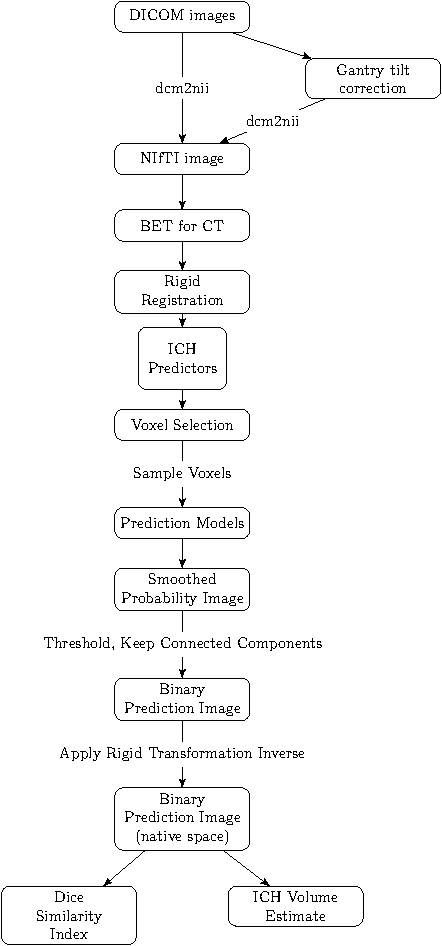
\includegraphics[width=0.5\linewidth]{Imaging_Pipeline_Flowchart_with_Rigid.pdf}
\caption{{\bf Processing Pipeline}.  Images in DICOM (Digital Imaging and Communications in Medicine) format were gantry tilt corrected if necessary and converted to NIfTI (Neuroimaging Informatics Technology Initiative) format using \texttt{dcm2nii}.  After NIfTI conversion, the brain extraction tool (BET) was applied to the image using a previously published protocol.  The image was rigidly registered to a brain CT template.  We estimated imaging predictors and used these predictors to estimate the probability of ICH in a prediction model.  The probability of ICH was thresholded, connected component below $100$ voxels ($0.1$mL) were discarded, and the image was transformed back into original space of the patient.  The ICH volume and the Dice Similarity Index, an overlap measure, were calculated compared to the true estimate from the manual segmentation.  }
\label{fig:framework}
\end{figure}

\subsection{Image Registration}
\citet{rorden_age-specific_2012} introduced a CT template based on $35$ individuals who presented with specific neurological deficits that were suspected to be caused by a stroke, but were later found to be due to a metabolic abnormality.  This CT template is represented in MNI (Montreal Neurological Institute) space and brain-extraction was performed on the template.  Prior to image processing, brain-extracted images were registered to this brain-extracted template using a rigid-body (6 degrees of freedom) and linearly interpolated to a $1\times1\times1$mm voxel resolution.  Transformed hemorrhage masks and brain masks were thresholded using a value of $0.5$ to preserve mask volume \cite{flirt_reg}. This operation reoriented the image, ensured isotropic voxel sizes for smoothing and other operations below, and preserved the relative volume of the ICH.  All image preprocessing and analysis are done in MNI space, described as template space, unless otherwise specified.


\subsection{Brain Mask Erosion}
Each brain mask was eroded by a box kernel ($3\times3\times1$mm).  Though this erosion may exclude voxels from superficial bleeds towards the cortical surface, it excludes voxels with similar ranges as ICH voxels, caused by 1) incomplete skull stripping or 2) partial voluming effects with the skull.  If any voxels from the hemorrhage mask was removed due to brain extraction or brain mask erosion, these voxels were included in estimating model performance but their predicted probability of ICH was set to $0$.  Therefore, these deleted ICH voxels will always be incorrectly predicted as not ICH.  

%This eroded mask and any excluded ICH voxels contained all voxels used for exploratory analysis and model fitting, which we will refer to as candidate voxels.



\subsection{Imaging Predictors}
We derived a set of imaging predictors from each CT scan.  We will describe each here with their rationale for use.  These features make up the potential set of predictors for image segmentation.
%Note that the corresponding images have roughly a distribution of between $0$ and $100$ HU as they have been skull stripped.  

\subsubsection{CT voxel intensity information} The raw voxel intensity value in HU was included $x(v)$, as it is the main predictor used in visual inspection; high HU values are indicative of hemorrhage. We created an indicator if the value was greater than $40$ and less than $80$ HU, similar to the criteria used for manual segmentation, denoted $I_{\text{thresh}}(v)$. 

\subsubsection{Local Moment Information} For each voxel, we extracted a neighborhood, denoted $N(v)$, of all adjacent neighboring voxels in $3$ dimensions and the voxel itself.  Let $x_k(v)$ denote the voxel intensity in HU for voxel neighbor $k$, where $k = 1, \dots, 27$.  We created the voxel neighborhood mean intensity ($\bar{x}(v)$):
\begin{equation}
\bar{x}(v) = \frac{1}{N(v)} \sum_{k \in N(v)} x_k(v) \label{eq:mean}
\end{equation}
We calculated the voxel neighborhood standard deviation (SD), skew, and kurtosis using the following method of moments estimators:
\begin{eqnarray*}
\text{SD}(v) &=& \sqrt{ \frac{1}{N(v)} \sum_{k \in N(v)} \left(x_k(v) - \bar{x}(v)\right)^2 } \\
\text{Skew}(v) &=& \frac{ \frac{1}{N(v)} \sum\limits_{k \in N(v)} (x_k(v)-\bar{x}(v) )^3 } {\left[ \frac{1}{N(v)} \sum\limits_{k \in N(v)} (x_k(v)- \bar{x}(v))^2\right]^{3/2}} \\
\text{Kurtosis}(v) &=& \frac{ \frac{1}{N(v)} \sum\limits_{k \in N(v)} (x_k(v)-\bar{x}(v) )^4 }{ \left( \frac{1}{N(v)} \sum\limits_{k \in N(v)} \left(x_k(v) - \bar{x}(v)\right)^2\right)^2} \\
\label{eq:moment}
\end{eqnarray*}
We acknowledge that we did not divide by $N(v) - 1$ for standard deviation and skew, nor did we subtract by $3$ for kurtosis.  As $N(v)$ should be the same per voxel, this should not affect the estimates for prediction: it will be accounted for in any generalized linear model by the intercept and scaling of the beta coefficients and a tree-based decision algorithm will simply have a different cutoff value for binning.

Voxels higher in their local mean correspond to voxels adjacent to higher HU voxels on average, which are more likely to be ICH.  The higher order moments can provide information about how homogeneous the intensities in the neighborhood are and where edges occur.  We also calculate the percentage of voxels in each neighborhood ($p_{\text{thresh}}(v)$) that have HU values between $40$ and $80$:
\begin{equation}
p_{\text{thresh}}(v) = \frac{1}{N(v)} \sum_{k \in N(v)} I\{ 40 \leq x_k(v) \leq 80 \} \label{eq:pct}
\end{equation}
which should be higher for ICH voxels as they are surrounded by high HU values.  

Voxels that are on the surface or surrounded by non-brain tissue are less likely to be ICH.  Voxels not within the eroded mask are set to $0$; the following predictors assume that voxels close to many voxels with intensity $0$ are less likely to be ICH.    
We calculated the percentage of voxels that have neighbors of value of $0$:
\begin{equation}
p_{0}(v) = \frac{1}{N(v)} \sum_{k \in N(v)} I\{ x_k(v) = 0 \} \label{eq:pct0}
\end{equation}
and an indicator of whether any voxels in the neighborhood had a value of $0$:
\begin{equation}
\bar{I}_{0}(v) = I\{ p_{0}(v) > 0 \} \label{eq:I0}
\end{equation}
 
\subsubsection{Within-plane Standard Scores} Some brain structures have high HU values but are not ICH, such as the falx cerebri, which lies largely on the mid-sagittal plane.  Moreover, tissues in the top of the brain may have a higher average HU than those in the middle or bottom of the brain.  Thus, if values are standardized within each plane (axial, sagittal, coronal), these standard-plane scores may distinguish high values within a plane regardless of a mean shift, which may indicate ICH voxels.

We created standard-plane scores for each voxel on a slice-based level for axial, sagittal, and coronal planes. For each plane $o \in \{$axial, sagittal, and coronal$\}$, we calculated the standard-plane score as follows: 
\begin{equation}
z_{o}(v) = \frac{x(v) - \bar{x}(v, o)}{\sigma(v, o)} \label{eq:z}
\end{equation}
where $\bar{x}(v, o)$ and $\sigma(v, o)$ denote the mean and standard deviation of plane $o$ which contains voxel $v$, excluding voxels outside the brain mask.   In addition to the standardized images within plane we created a Winsorized standardized image, using the Winsorized mean and standard deviation, with a 20\% trimming of the distribution, which may allow for better standardization with artifacts of the distribution (such as gross hyperintensities). 

\subsubsection{First-pass Segmentation} We used a previously-published, open-source, general segmentation tool based on Markov random fields for image segmentation, called Atropos \citep{atropos}.  We used a 4-tissue class segmentation, and added the top probability values from the top 2 classes to combine them into one class.  We used this probability image as a predictor, denoted by $\text{prior}(v)$.  Although this tool has been shown to perform well in other studies for tissue-class segmentation, it did not perform adequately as a standalone segmentation tool for ICH in CT.  

\subsubsection{Contralateral Difference Images}  As most hemorrhages are constrained to one side of the brain, the contralateral side should have lower HU values.  For non-hemorrhage voxels, however, the contralateral voxels would have similar HU values, and thus their difference would be small or negative.  Thus, we right-left flipped the image, and took a difference image: 
\begin{equation}
f(v) = x(v) - x(v^{*}) \label{eq:flip}
\end{equation}
where $v^{*}$ is the voxel from the contralateral side.  



\subsubsection{Global Head Information} We used the distance to the brain centroid ($d(v)$) to potentially down-weight voxels that are very far from the brain center, which may be artifacts.    We also created $3$ images that were obtained by smoothing the original image using large Gaussian kernels ($\sigma = 5mm^3, 10mm^3, 20mm^3$), which can capture any potential homogeneity throughout the scan, denoted by $s_{5}(v)$, $s_{10}(v)$ and $s_{20}(v)$, respectively.   

\subsubsection{Standardized-to-template Intensity}  
Although standardizing voxels compared to within-scan measurements can detect anomalous tissue, one powerful tool is to use a measure how different a voxel is compared to that voxel in a person from a non-stroke population.  We registered the brain-extracted image to the brain-extracted CT template using an affine transformation, followed by a non-linear transformation estimated using Symmetric Normalization (SyN) \citep{avants_symmetric_2008}.  
From $30$ CT images from non-stroke patients from Dr.~Rorden (personal communication), we registered these non-stroke, brain-extracted scans to the CT template, and created a voxel-wise mean image $M$ and voxel-wise standard deviation $S$ image in template space.  For each scan in our study, we created a standardized voxel intensity with respect to this population ($z_{\text{template}}$) using the following equation:
$$
z_{\text{template}}(v) = \frac{x(v) - M(v)}{S(v)}
$$
This image is warped back into the rigid-body-registered space so that these standardized voxels are aligned with other predictors.  This predictor is similar to that used in \citet{gillebert_automated_2014}.  


\begin{figure}
\centering
\begin{center}
\begin{tabular}{@{}c@{}c@{}c@{}c@{}}
$x(v)$ & Atropos $\text{prior}(v)$ & $f(v)$ & $d(v)$ \\
\makeimg{\mywidth}{_SS} & \makeimg{\mywidth}{_prob_img} & \makeimg{\mywidth}{_flipped_value}   & \makeimg{\mywidth}{_dist_centroid} \\
$\bar{x}(v)$ & $\text{SD}(v)$ & $\text{Skew}(v)$ & $\text{Kurtosis}(v)$\\
\makeimg{\mywidth}{_moment1} & \makeimg{\mywidth}{_moment2} &  \makeimg{\mywidth}{_skew} &  \makeimg{\mywidth}{_kurtosis}\\
$p_{0}(v)$ & $\bar{I}_{0}(v)$  & $p_{\text{thresh}}(v)$ & $I_{\text{thresh}}(v)$\\
\makeimg{\mywidth}{_pct_zero_neighbor} & \makeimg{\mywidth}{_any_zero_neighbor} & \makeimg{\mywidth}{_pct_thresh_40_80} & \makeimg{\mywidth}{_thresh_40_80}   \\
$s_{5}(v)$ & $s_{10}(v)$  & $s_{20}(v)$& $z_{\text{template}}(v)$ \\
\makeimg{\mywidth}{_smooth5}  & \makeimg{\mywidth}{_smooth10} & \makeimg{\mywidth}{_smooth20} & \makeimg{\mywidth}{_zscore_template} 
\end{tabular}
\end{center}
\caption{{\bf Predictor Images}. Here we display one slice from one patient for predictor images.  
The within-plane and Winsorized predictor images were not shown as they are within-subject scaled version of the image $x(v)$ and would appear very similar.  Although they appear similar at a subject level, the distribution of these predictors is different across patients.  The images that visually separate the areas of ICH compared to the rest of the image are likely to be better predictors. 
}
\end{figure}




%To further illustrate how smoothing affects brain extraction, we present one example case where brain extraction performance with BET was acceptable only after smoothing.  





\subsection{Voxel Selection Procedure}
We chose $10$ scans from $10$ patients to perform exploratory data analysis, model fitting, and estimation of model cutoffs, denoted as training data. We used the $102$ remaining scans as test data to estimate performance.
%Of the non_nmods remaining scans, we split the data into $groups["Validation"]$ validation scans and  $groups["Test"]$ test scans.  


From the training data we estimated the $0.5\%$ and $99.5\%$ quantiles for all ICH voxels in the predictors.  Voxels that were jointly within these quantiles for $z_{\text{axial}}$, $z_{\text{coronal}}$, $p_{\text{thresh}}$, and within HU between $30$ and $100$ were considered candidate voxels of ICH; voxels outside of the intersection of these ranges were given a $0$ probability of ICH. These cutoffs empirically found to be robust in the test scans; they excluded a mean 63.6 (min: 37.1, max: 89.8) percentage of non-ICH voxels, while including a mean 97.9 (min: 91.6, max: 99.9) percentage of ICH voxels.  This voxel selection procedure should improve the specificity of model predictions, and improve computational speed.  

\subsection{Models}

From these 10 scans, we collapsed all the voxels passing the voxel selection procedure.  From these voxels, we randomly sampled $100{,}000$ to fit the models and do data exploration, and used the remaining voxels to estimate the model cutoffs of the probability of ICH.   All models were fit with all predictors.  

% get Reseg_Aggregate_data Rda for nunmber of voxels 

Using the sampled training voxels, we created predictions for the probability of ICH using a 1) logistic regression model, 2) logistic regression model with a penalty, 3) generalized additive model (GAM), and 4) classifier fit with the random forest algorithm.

For the standard and penalized logistic regression model, we used all predictors.  The penalized model was fit using the LASSO (Least Absolute Shrinkage and Selection Operator) penalty \citep{tibshirani_regression_1996} using the \pkg{glmnet} package \citep{friedman_regularization_2010}.  The tuning parameter ($\lambda$) for the penalization was chosen using 10-fold cross-validation (of only the training voxels in the model), with the cost function of misclassification rate.  The parameter was chosen using the largest value of $\lambda$ such that the error is within 1 standard error of the minimum, chosen for out-of-sample performance stability.

The generalized additive model (GAM) \citep{hastie_generalized_1986, hastie_generalized_1990} was also created using indicator variables for binary variables and thin-plate splines for all continuous measures, fit with fast-estimation of restricted maximum likelihood (fREML) using the \pkg{mgcv} package \citep{wood_fast_2011, wood_generalized_2015}.   Model specifications can be seen in Section~\ref{sec:modspec}.


We fit a random forest \citep{breiman2001random} using the \pkg{randomForest} package in R \citep{randomForest}, using the default pruning parameters and number of trees (\code{ntree=500}, \code{mtry=4}). 



\subsection{Estimating a Cutoff for Model Probability}

Each model gives the estimate of the probability a voxel is ICH.  In the end, however, we want a predicted binary hemorrhage mask to compare to the manual segmentation. 
Using the voxels from the training data, we estimated the probability of ICH from each model.  For each model probability, we smoothed this probability image using the neighborhood voxels (1 voxel in every direction).  To choose a probability cutoff to make a binary image, we used the voxels in the training data that were not sampled for estimating the model.  Using these voxels in the smoothed images, we estimated the probability cutoff that minimized the Dice Similarity Index (DSI) \citep{dice_measures_1945} between the prediction and true value.  
 The DSI is measure of overlap insensitive to values where neither the true segmentation nor predicted segmentation were considered ICH, and will be used as a performance measure when comparing models.  DSI for scan $i$ is calculated by 
 $$
 DSI_i = \frac{2 \times TP}{2\times TP + FN + FP}
 $$
 where $TP$ denotes the number of ``true positives'', where the manual and predicted segmentation are both $1$, $FP$ denotes the number of ``false positives'', where the manual segmentation is $0$ and predicted segmentation is $1$, and $FN$ denotes the number of ``false negatives'', where the manual segmentation is $1$ and predicted segmentation is $0$.  DSI ranges from $0$ to $1$; $0$ indicates no overlap and $1$ denotes perfect overlap.

After thresholding the smoothed image using this probability cutoff, we discarded regions with fewer than $100$ ($0.1$mL) connected voxels.  We then transformed this binary mask back to original (i.e.~native) space using the inverse from the previously estimated rigid-body transformation.  As the linear interpolation results in a non-binary mask, we thresholded this image at $0.5$ to preserve volume \cite{flirt_reg}.  

For each scan in the test data, this voxel selection and prediction process was performed and each scan has a corresponding binary prediction  image.  For evaluation of all measures, the comparison was done in the native space of the patient, not in the template space, as this was where the manual segmentation was done.


\subsection{Measuring and Testing ICH Prediction Performance}





For all measures, we used the binary prediction masks from the test scans.  We measured performance for each model using the DSI and also estimated the ICH volume of the prediction. The number of true negatives inflates specificity and overall accuracy, since most of the voxels within the brain are non-ICH, and are not reported.  We tested the difference between median DSI across models using a Kruskal-Wallis test.  If a difference was present, we tested each combination of models ($6$ combinations) using a Wilcoxon signed rank test, and corrected the p-value using a Bonferroni correction.


We also calculated the relationship of estimated volume of ICH compared to the manual segmentation using the Pearson correlation and root mean squared (RMSE) between volumes measures.  Similarly, we did performed a Kruskal-Wallis test on the medians of the absolute value of the difference in estimated volume from each model and the true volume and performed pairwise tests if necessary.  For DSI and correlation, higher values indicate better agreement with the manual segmentation.  For RMSE, lower indicates better agreement.


\section{Results}

\subsection{Dice Similarity Index}
In Figure~\ref{fig:dice}, we show the DSI distributions from the test data for each model.  We see that DSI is high on average for all models, with a few scans having a very small DSI (i.e.~failures).   The median DSI for each model was: $0.89$ (logistic), $0.885$  (LASSO), $0.88$ (GAM), and $0.899$ (random forest). 
We also note that using the random forest results in a slightly higher median DSI compared to the other models, and there was a difference across medians ($\chi^{2}(3)=13.49$, $p < 0.05$).  Indeed, after Bonferroni correction, the only comparisons that were significant were comparing the random forest DSI to the DSI from the logistic ($p < 0.001$), LASSO ($p < 0.001$), or GAM ($p < 0.001$) models.

In Figure~\ref{fig:dice_img}, we display the CT scan of the patient in the test data that has the median DSI in the test scans. The image depicts the brain-extracted CT scan and then the CT scan with overlaid colors.  The green indicates a correct classification of ICH from the model (true positive), blue indicates a false negative, and red indicates a false positive.  Note, the image has finer resolution in the axial slice ($0.5$mm by $0.5$mm) than in the inferior/superior planes ($5$mm), as is commonly used for radiological evaluation of hemorrhages.  Patients with the lowest, $25^{\text{th}}$, $75^{\text{th}}$, and highest DSI are shown in Supplemental Figures~\ref{fig:dice_img0}, \ref{fig:dice_img25}, \ref{fig:dice_img75}, and \ref{fig:dice_img100}, respectively.



\begin{figure}
\centering
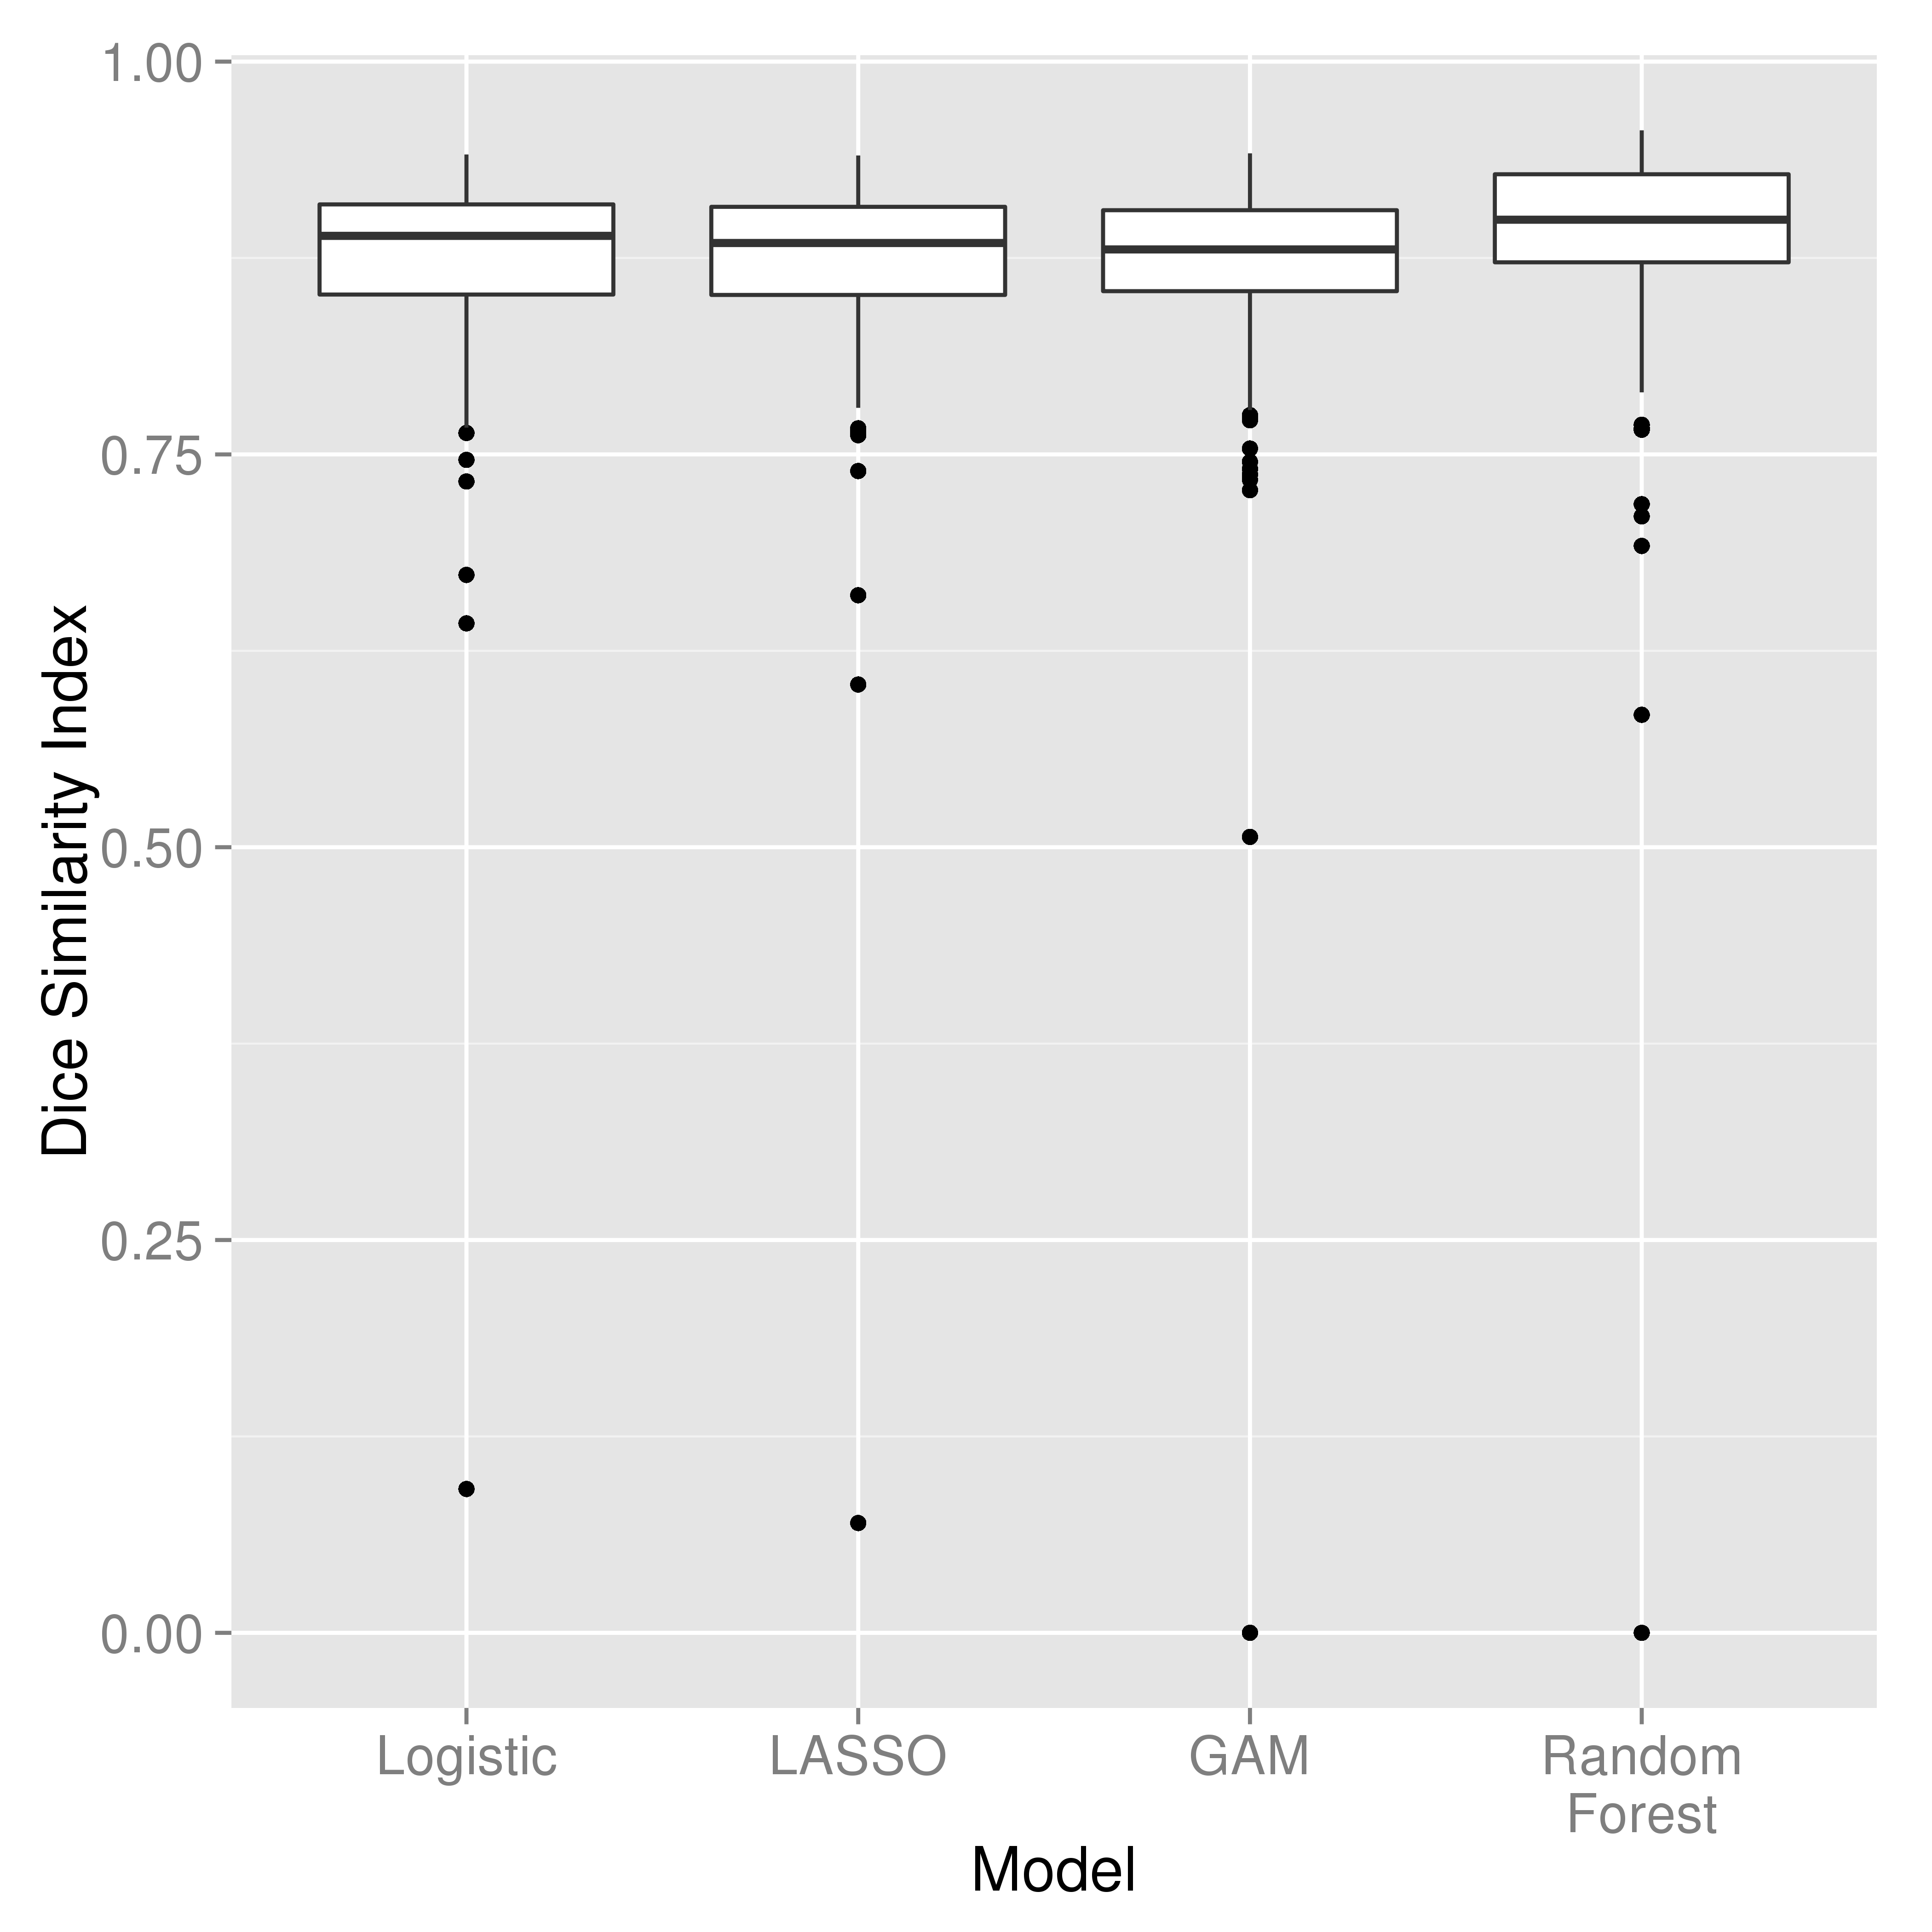
\includegraphics[width=0.75\linewidth,keepaspectratio]{Reseg_Dice_Comparison.png}
\caption{{\bf Distribution of Dice Similarity in Test Scans}.  Here we display the boxplot of the Dice Similarity Index (DSI), a measure of spatial overlap between the estimated hemorrhage mask and the manually-delineated hemorrhage mask, in the $102$ test scans.  We present the DSI distribution for each model fit: a logistic regression, a logistic model penalized with the Least Absolute Shrinkage and Selection Operator penalty (LASSO), a generalized additive model (GAM), and a random forest algorithm.  Overall, we see high agreement between the manual and estimated hemorrhage masks with the median of $0.89$ for the logistic model, $0.885$ for the LASSO, $0.88$ for the GAM, and $0.899$ for the random forest. The median DSI for the random forest was significantly higher than those of the other 3 models, after adjusting for multiplicity using a Bonferroni correction (all $p < 0.05$).   }
\label{fig:dice}
\end{figure}



\begin{figure}
\centering
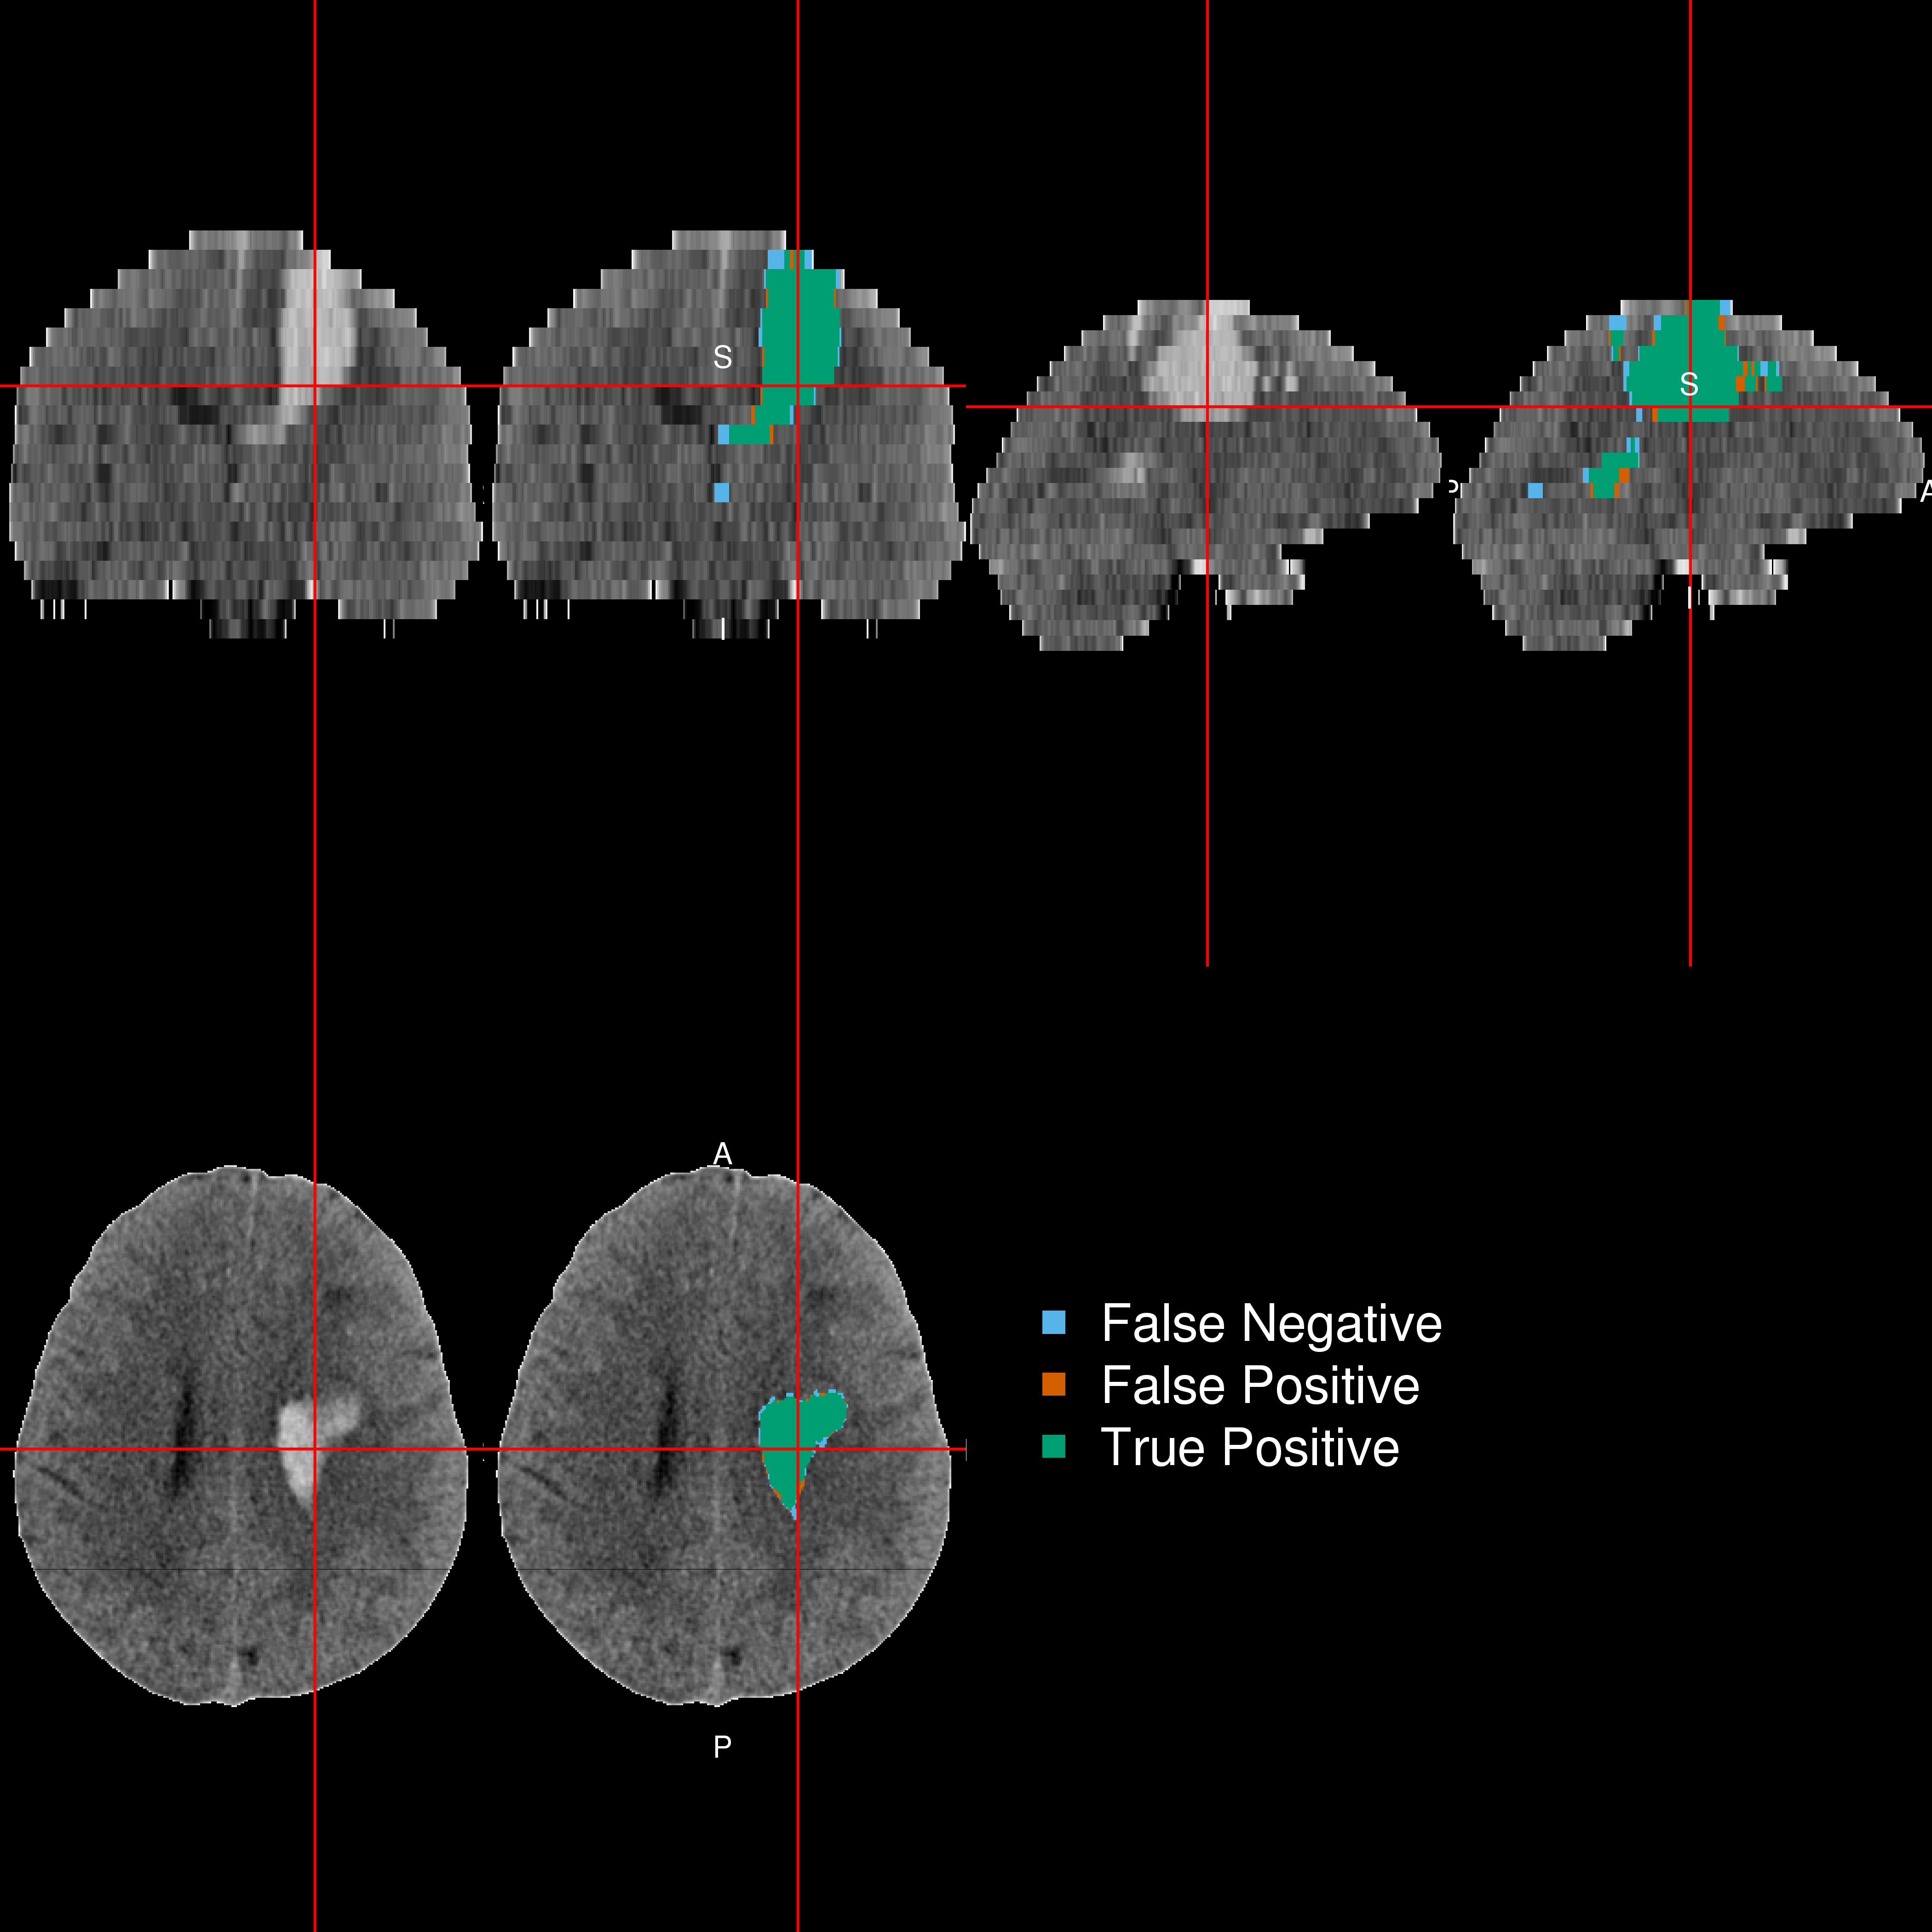
\includegraphics[width=0.75\linewidth,keepaspectratio]{Reseg_Figure_DSI_Quantile_050_native.png}
\caption{{\bf Patient with Median Dice Similarity Index}. We present the patient with the median Dice Similarity Index (DSI), a measure of spatial overlap, from the chosen predictor model fit with a random forest.  The median DSI was $0.899$, which indicates high spatial overlap. The green indicates a correct classification of ICH from the model, blue indicates a false negative, where the manual segmentation denoted the area to be ICH but the predicted one did not, and red indicates a false positive, where the predicted segmentation denoted the area to be ICH but the manual one did not. }
\label{fig:dice_img}
\end{figure}

\subsection{ICH Volume Estimation}
In Figure~\ref{fig:vol}, we show the estimated ICH volume versus that from the manual segmentation.  The pink line represents the $X = Y$ line, where the estimated and true volume are identical.  The blue line represents the linear fit; the line equation and correlation are printed on the plot.  The farther away the slope of the equation is from $1$ represents a multiplicative bias, where values greater than $1$ represents larger estimated volumes.  The farther the intercept is from $0$ represents and additive bias in the estimated volume, where values greater than $0$ again represent larger estimated volumes.  The correlation (95\% confidence interval (CI)) between the true volume and the volume predicted volume were $0.92$ (95\% CI: $0.884, 0.945$) for the logistic model, 
$0.916$ ($0.878, 0.942$) for the LASSO, 
$0.908$ (95\% CI: $0.866, 0.937$) for the GAM, and  
$0.932$ (95\% CI: $0.901, 0.954$) for the random forest.  The RMSE for all the logistic (RMSE: $10.67$ mL), LASSO ($10.83$ mL), and random forest ($10.27$ mL) models, but was slightly higher for the GAM model ($11.36$ mL).  The  Kruskal-Wallis test indicated no significant difference in the median absolute value of the difference in estimated versus true volume over models ($\chi^{2}(3)=2.3$, $p = 0.51$).  



\begin{figure}
\centering

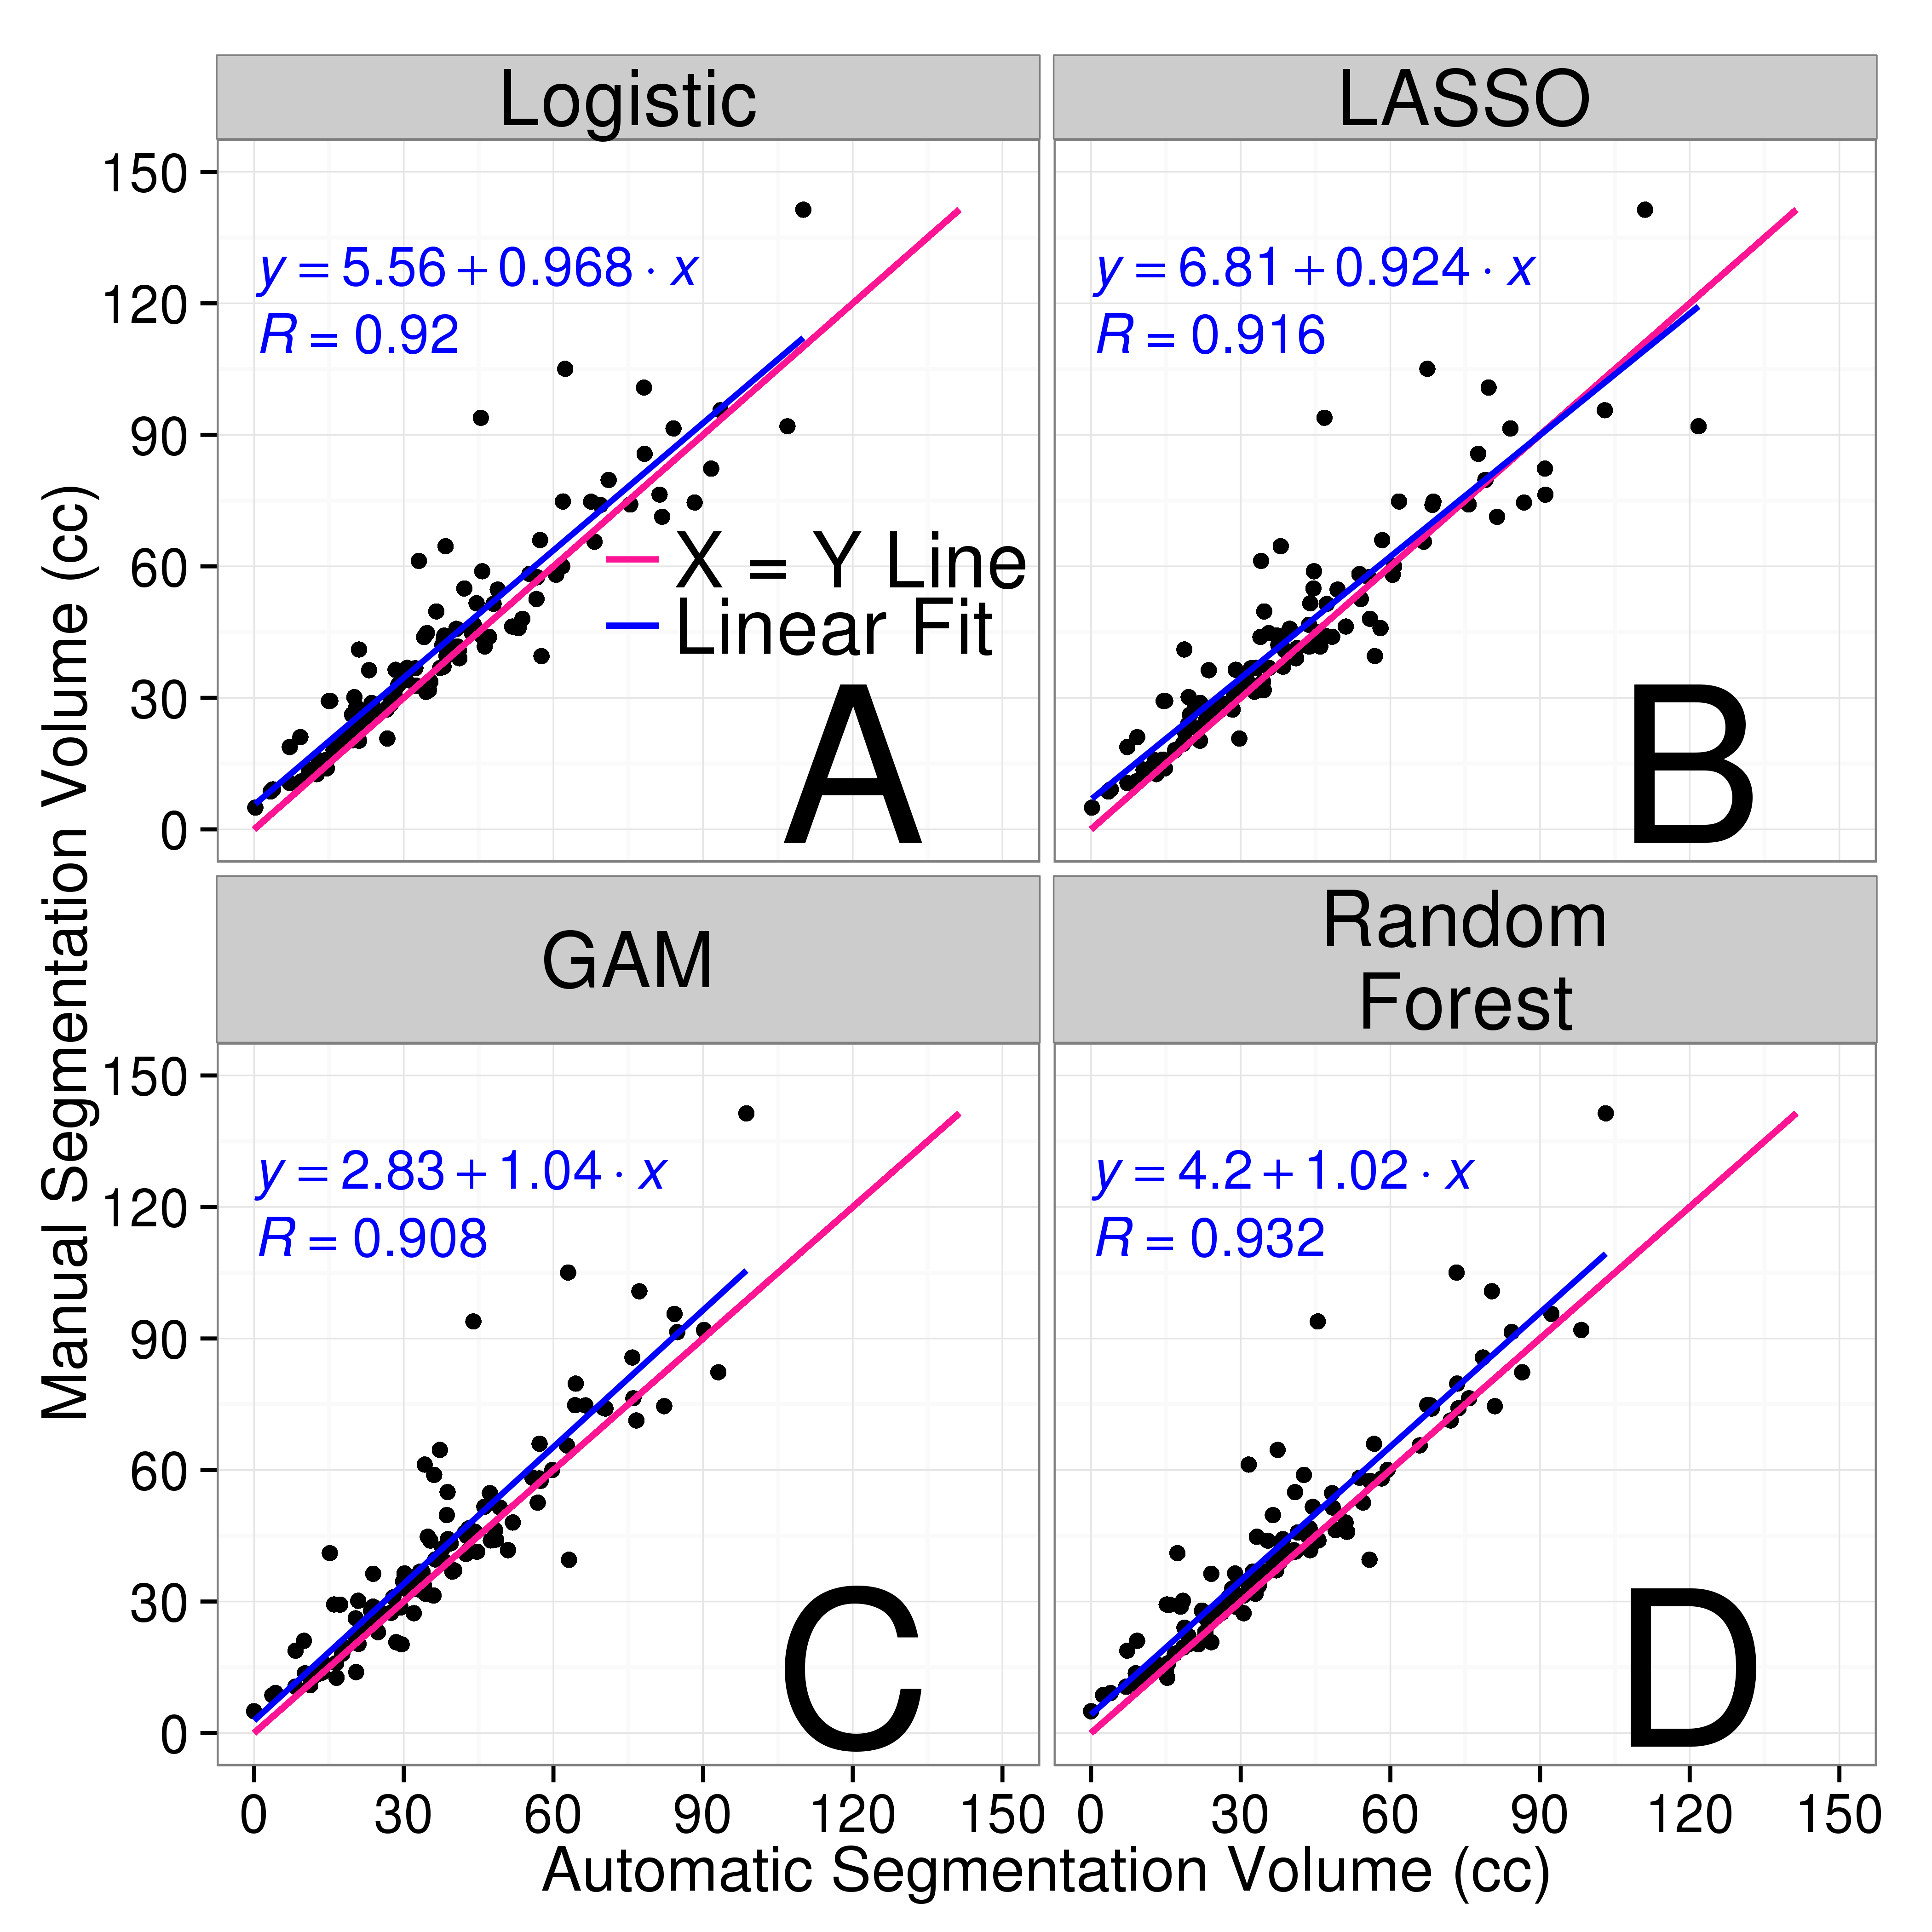
\includegraphics[width=\linewidth,keepaspectratio]{Reseg_Volume_Comparison.png}
\caption{{\bf Comparison of Estimated and Manual Intracerebral Hemorrhage Volume for Each Model}.  In each panel, we show the volume of intracerebral hemorrhage (ICH) estimated from each model (x-axis) versus that from the gold-standard manual segmentation (y-axis) in the $102$ test scans.  The pink line represents the $X=Y$ line, which represents perfect agreement.  The blue line represents a linear fit of the data, and the estimated slope equation is displayed along with the Pearson correlation.  Panel A represents the volume from the logistic regression model, B represents that from logistic model penalized with the LASSO, C represents that from a generalized additive model (GAM), and D represents that from a random forest algorithm.  Overall, we see high agreement between the estimated volume from automated segmentation from each model as all correlations are above $0.9$.  The farther away the slope of the equation is from $1$ represents a multiplicative bias, where values greater than $1$ represents larger estimated volumes.  The farther the intercept is from $0$ represents and additive bias in the estimated volume, where values greater than $0$ again represent larger estimated volumes.  }
\label{fig:vol}
\end{figure}

\subsection{Model Choice}
Overall, all models perform well for ICH segmentation.  Some failures exist, but the algorithm using the random forest to fit the probability of ICH had higher median DSI, the lowest RMSE, and the highest correlation compared to the other models.  Therefore, when implementing the algorithm, the model used will be the random forest.



\section{Discussion}
We have presented a novel, fully automated method for segmentation of ICH from CT scans. Our method uses only CT scans from patients with stroke as additional information from MRI was not standardized nor is the standard of care with the disease. We validated this method against the manual segmentation of ICH as a gold standard.  We used the Dice Similarity Index and correlation between the volume of ICH from manual and automatic segmentation as measures to determine how well an algorithm performed.  

We create a set of predictors that attempt to capture the features relevant to distinguishing ICH versus non-ICH areas and described the rationale for each predictor.  We have used these predictors in a series of models, including those fit with logistic regression, logistic regression penalized with the LASSO, generalized additive models, and random forests.  All models result in high values for the DSI and high correlations for the volume of ICH from manual and automatic segmentation. Estimating the probability of ICH using random forests appeared was chosen as the final algorithm based on DSI; that algorithm also had high correlations of automated versus manual ICH volume.  

Comparing the manual to the automatic segmentation in each quantile of DSI showed that some cases may fail ($N = 1$ with DSI below $0.5$), but much of the discrepancy occurs at the edges of the hemorrhage.  This may be due to the smoothing operations performed in the model, which are isotropic and do not preserve edges.  Anisotropic smoothing, such as those presented in \citet{perona1994anisotropic}, may help preserve edges and result in better segmentation.  



Other methods have been presented for segmentation of ICH from CT scans \citep{ gillebert_automated_2014, prakash_segmentation_2012, loncaric_hierarchical_1996, loncaric_quantitative_1999, perez_set_2007}.  \citet{loncaric_hierarchical_1996} performed an analysis on only one 2-dimensional scan and could not be compared.  The method in \citet{perez_set_2007} was semiautomated and was validated by visual inspection, which did not succeed in $6$ out of $36$ scans ($16.7\%$).  If we use the criteria of a DSI below $0.5$ as a failure, we had $1$ fail out of $102$ test scans ($1\%$).  We have higher median DSI ($0.899$) than those reported in \citet{gillebert_automated_2014} (approximately $0.62$ and $0.78$ for hemorrhagic strokes from graphs) and were comparable to \citep{prakash_segmentation_2012} ($0.897$, $0.858$, and $0.9173$ for different groups with hemorrhage). \citet{loncaric_quantitative_1999} did not compare hemorrhage masks to the manual segmentation, but compared ICH volumes on the manual and automatic segmentation on $5$ subjects measured $3$ times, which had a Pearson correlation of $0.917$ on all $15$ scans, similar to that reported from the random forest model selected above (R = $0.932$).  

Only \citet{gillebert_automated_2014} responded with any requests for software to perform the segmentation.  Although we believe that the method from \citet{gillebert_automated_2014} is comparable, it has not been packaged for general use.  As the analysis above was done in R, we have released a package that can perform ICH segmentation (\url{https://github.com/muschellij2/ichseg}), 
including the models for prediction, CT template from \citet{rorden_age-specific_2012}, standardized mean and standard deviation images, and functions to register the images, create the predictors, predict from the models, and return a binary hemorrhage mask.  Although a package is ideal for prediction on a large number of images, we believe that this limits those who can test or try the software.  Therefore, we have released a Shiny \citep{shiny} R application online (\url{http://bit.ly/ICH_SEG}) for researchers to input CT scans and the application will output ICH segmentation masks, while giving an image depicting each processing step.  

One of the potential concerns with image registration with patients with ICH is image registration.  Although this method uses non-linear registration for one predictor, the standardized-to-template intensity, this predictor is transformed back to the rigid-to-template space after standardization.  The method generally relies only rigid-body registration to a template.  This registration is largely done for head reorientation and resampling to isotropic voxel sizes across patients.  Thus, when morphological operations  are performed, such as smoothing using millimeter specifications, they do not depend on the original voxel sizes.  Although the models were fit in the rigid-to-template space, voxels from the same space in template space are not compared across patients in the models.  Also, the method returns hemorrhage masks in the native space of the patient, so they are easily comparable to any segmentation method performed on the original scan, such as clustering.  Thus, we use non-linear registration in one step, but do not rely on highly accurate image registration for comparability of voxels across patients, which can be problematic with patients with large hemorrhages.


Another concern from the process above is that the algorithm was only fit on $10$ patient scans.  Moreover, it was only fit with the sampled $100{,}000$ voxels that passed the voxel selection procedure from these scans.  Although this is a small sample, the models have shown to have high out-of-sample accuracy.  As this was the original procedure done, the training and test sets were not changed after this analysis to help avoid overfitting the models to the test set.  If a cross-validation approach was done across the entire set of scans,  the models must also be combined in some way to give a final prediction.  Validation of this method on additional data is required, but the test scans used are from multiple sites, different scanners, and have patients with heterogeneous hemorrhages both heterogeneous in size and location.  Thus, we believe this method to have good out-of-sample accuracy in a similar population.

As the process results in binary hemorrhage masks, one can use methods described in \citet{muschelli2015quantitative} to estimate quantitative measures of hemorrhage location.  Other automated analysis of hemorrhages can be done, such as shape analysis, which could not be done without a binary mask.  Overall, this process allows for researchers to use these hemorrhage masks for other voxel-based analyses that can yield novel insights into the relationship between hemorrhage characteristics and patient outcomes.

%Overall, the DSI results indicate good overlap between the predicted ICH segmentation and manual ICH segmentation on average with few failures.  Some non-contiguous areas may not be accurately segmented, but the estimate if ICH volume, which is used in prognostic models for stroke function outcome is accurate.


\subsection{Conclusions}
We have implemented and validated a fully automated segmentation algorithm of ICH in CT scans.  The method relies on series of processing steps and  creating a set of relevant predictors based on morphological operations such as smoothing, registration, and intensity normalization.  This method has been shown to agree with the gold standard of manual delineation of hemorrhages.  As an automated process, it is faster, does not require extensive radiologic image experience, is scalable to thousands of images, and does not have inter-reader variability.  As the process results in binary hemorrhage masks, one can then use these to define or test characteristics of ICH compared to patient-level information, such as those described in \citet{muschelli2015quantitative}) to estimate quantitative measures of hemorrhage location.  Most importantly, the volume of ICH is automatically calculated and can be used as a covariate in analysis, as this has been shown to be associated with long-term functional outcome \citep{broderick_volume_1993, jordan2009intracerebral, tuhrim_volume_1999}.  


\section*{Acknowledgments}
We would like to thank the patients and families who volunteered for this study, Genentech Inc. for the donation of the study drug (Alteplase), and the readers who manually segmented the ICH.  Dr. Chris Rorden was also extremely helpful in adapting his \code{dcm2nii} software to some issues specific to CT scans.

\section*{Sources of Funding}
The project described was supported by the NIH grant RO1EB012547 from the National Institute of Biomedical Imaging And Bioengineering, T32AG000247 from the National Institute on Aging, R01NS046309, RO1NS060910, RO1NS085211, R01NS046309, U01NS080824 and U01NS062851 from the National Institute of Neurological Disorders and Stroke, and RO1MH095836 from the National Institute of Mental Health. Minimally Invasive Surgery and rt-PA in ICH Evacuation Phase II (MISTIE II) was supported by grants R01NS046309 and U01NS062851 awarded to Dr. Daniel Hanley from the National Institutes of Health (NIH)/National Institute of Neurological Disorders and Stroke (NINDS).  Minimally Invasive Surgery and rt-PA in ICH Evacuation Phase III (MISTIE III) is supported by the grant U01 NS080824 awarded to Dr. Daniel Hanley from the National Institutes of Health (NIH)/National Institute of Neurological Disorders and Stroke (NINDS). Clot Lysis: Evaluating Accelerated Resolution of Intraventricular Hemorrhage Phase III (CLEAR III) is supported by the grant U01 NS062851 awarded to Dr. Daniel Hanley from the National Institutes of Health (NIH)/National Institute of Neurological Disorders and Stroke (NINDS). 

\newpage
%\section*{References}
%\bibliographystyle{elsarticle-num-names}
%\bibliography{CT_ICH_Segmentation}
%\bibliography{CT_Skull_Stripping_Bib}
\printbibliography

\clearpage
\section{Supplemental Material}

\subsection{Examples of Dice Similarity Index in Test Scans}

\begin{figure}
\centering
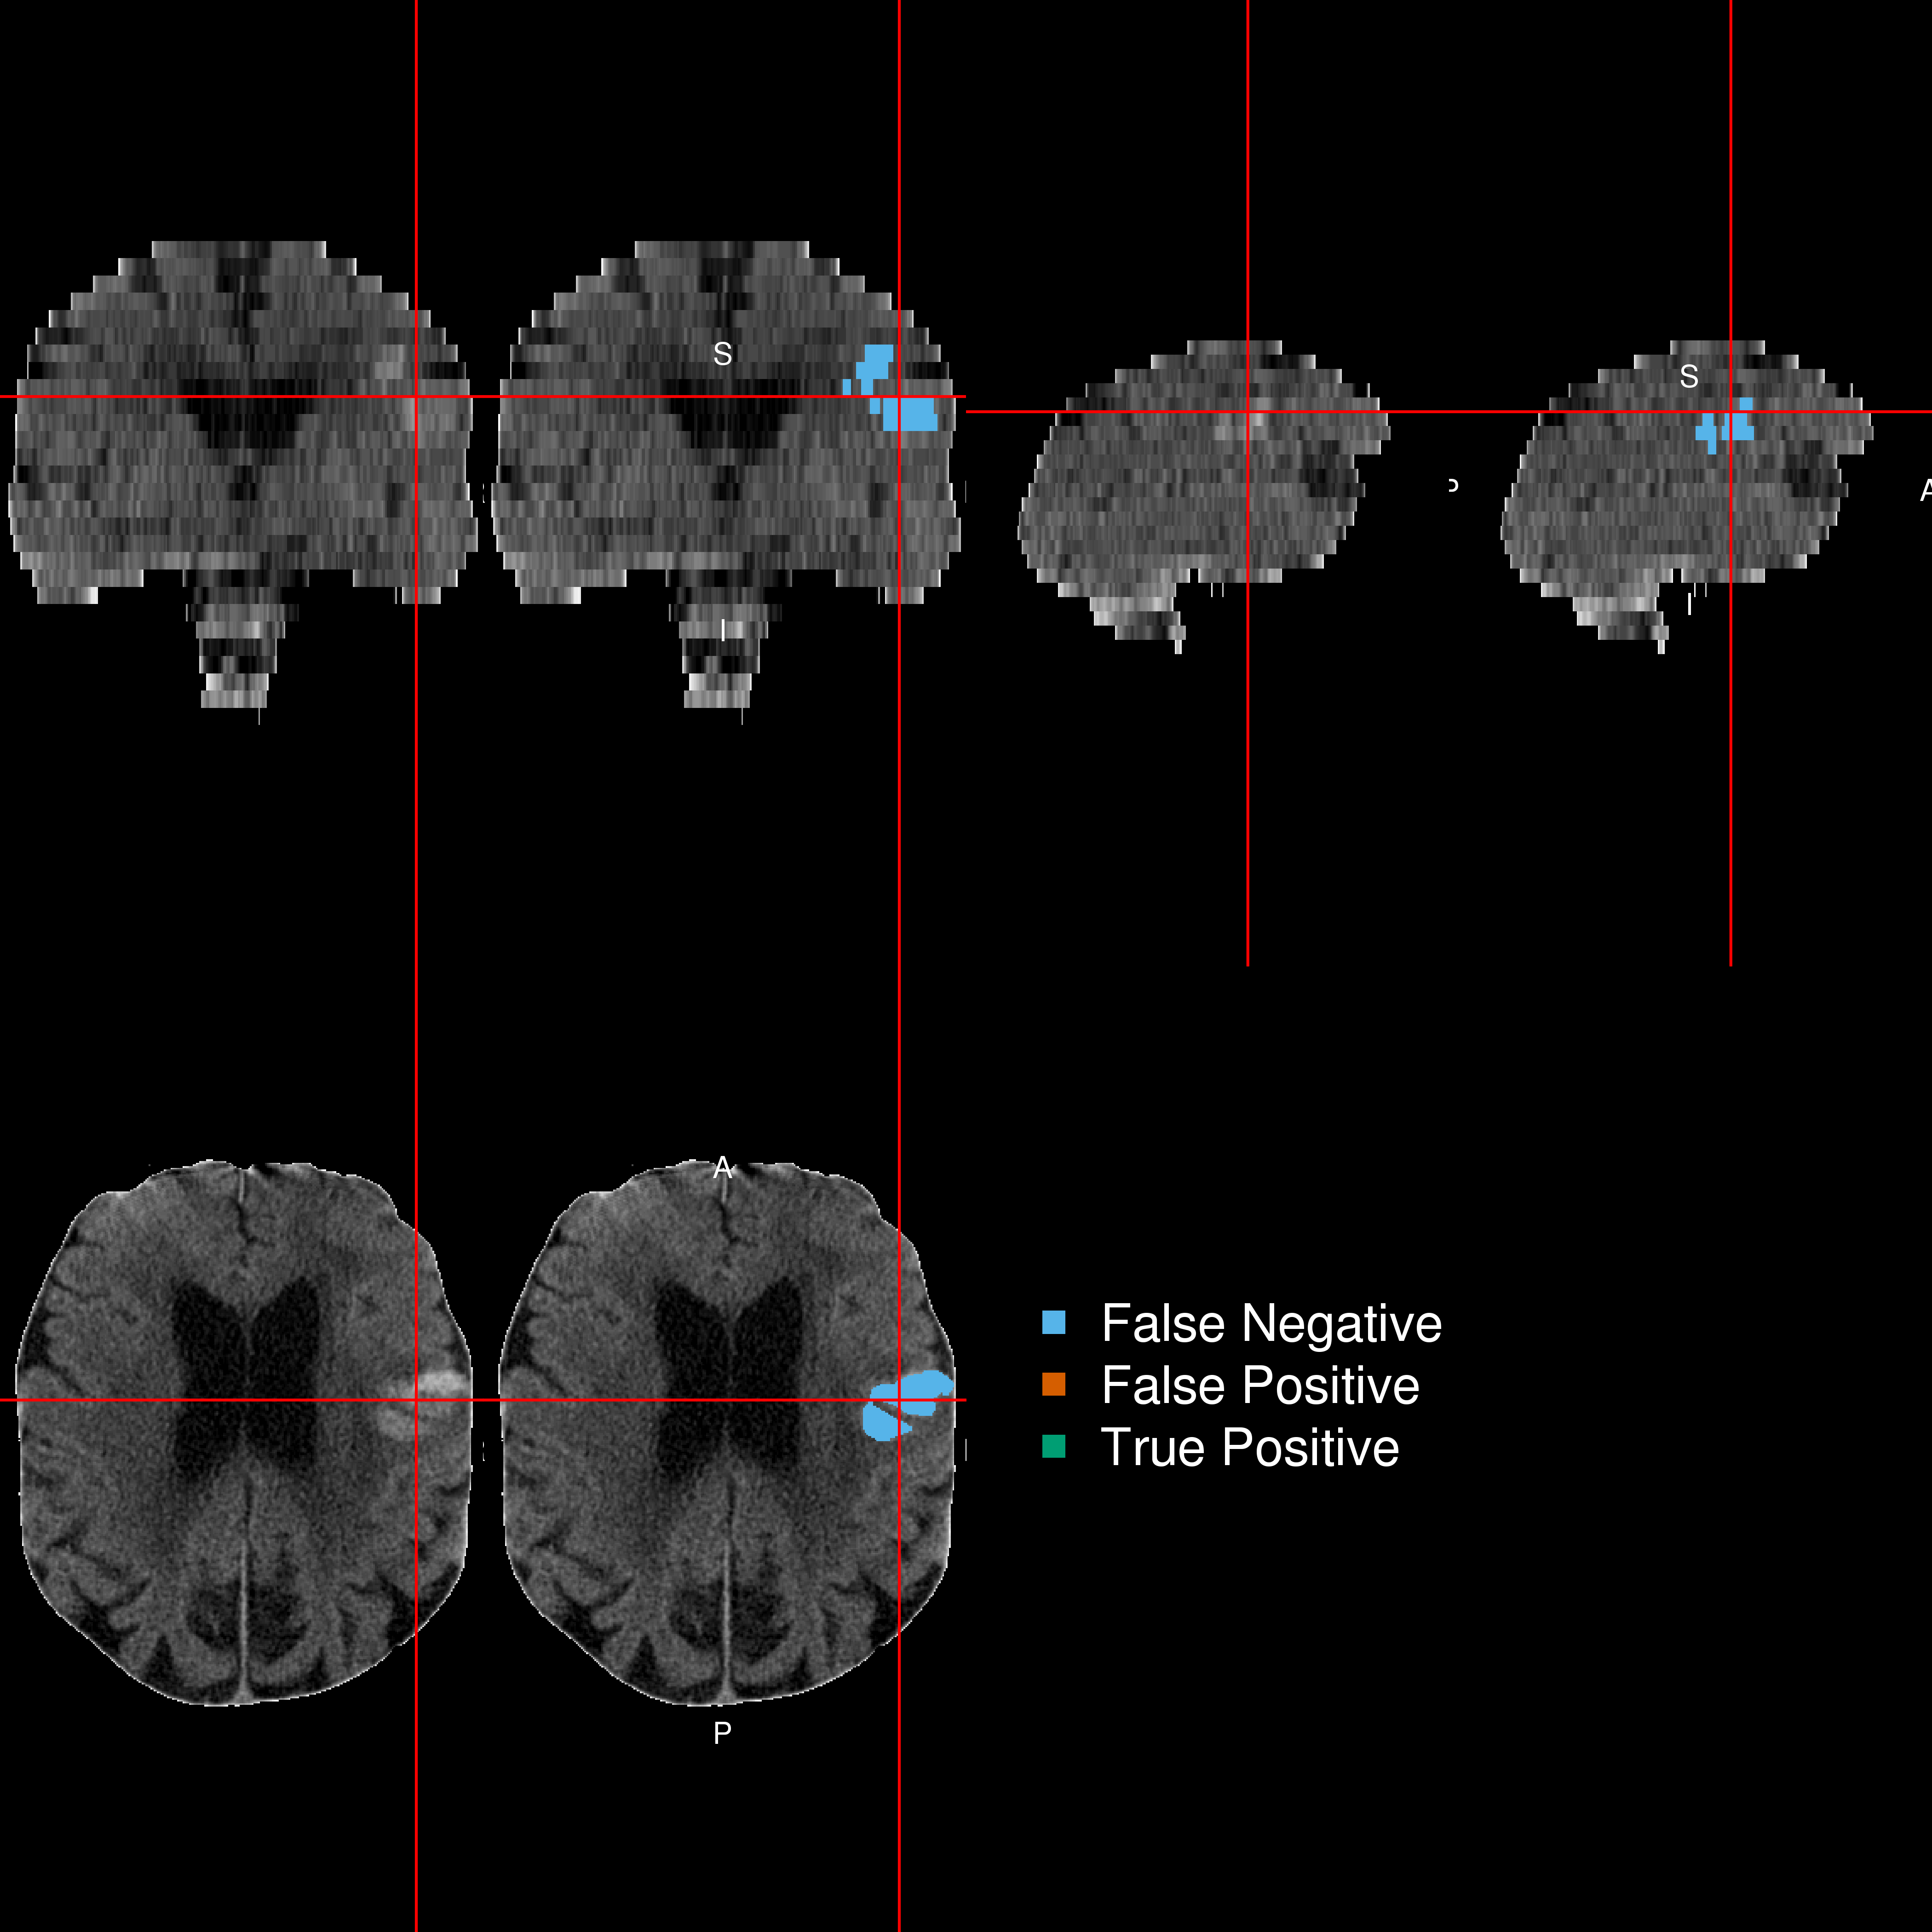
\includegraphics[width=0.75\linewidth,keepaspectratio]{Reseg_Figure_DSI_Quantile_000_native.png}
\caption{{\bf Patient with  Lowest Dice Similarity Index}. We present the patient with the lowest Dice Similarity Index (DSI), a measure of spatial overlap, from the chosen predictor model fit with a random forest.  The lowest DSI was 0. The green indicates a correct classification of ICH from the model, blue indicates a false negative, where the manual segmentation denoted the area to be ICH but the predicted one did not, and red indicates a false positive, where the predicted segmentation denoted the area to be ICH but the manual one did not. }
\label{fig:dice_img0}
\end{figure}

 \begin{figure}
\centering
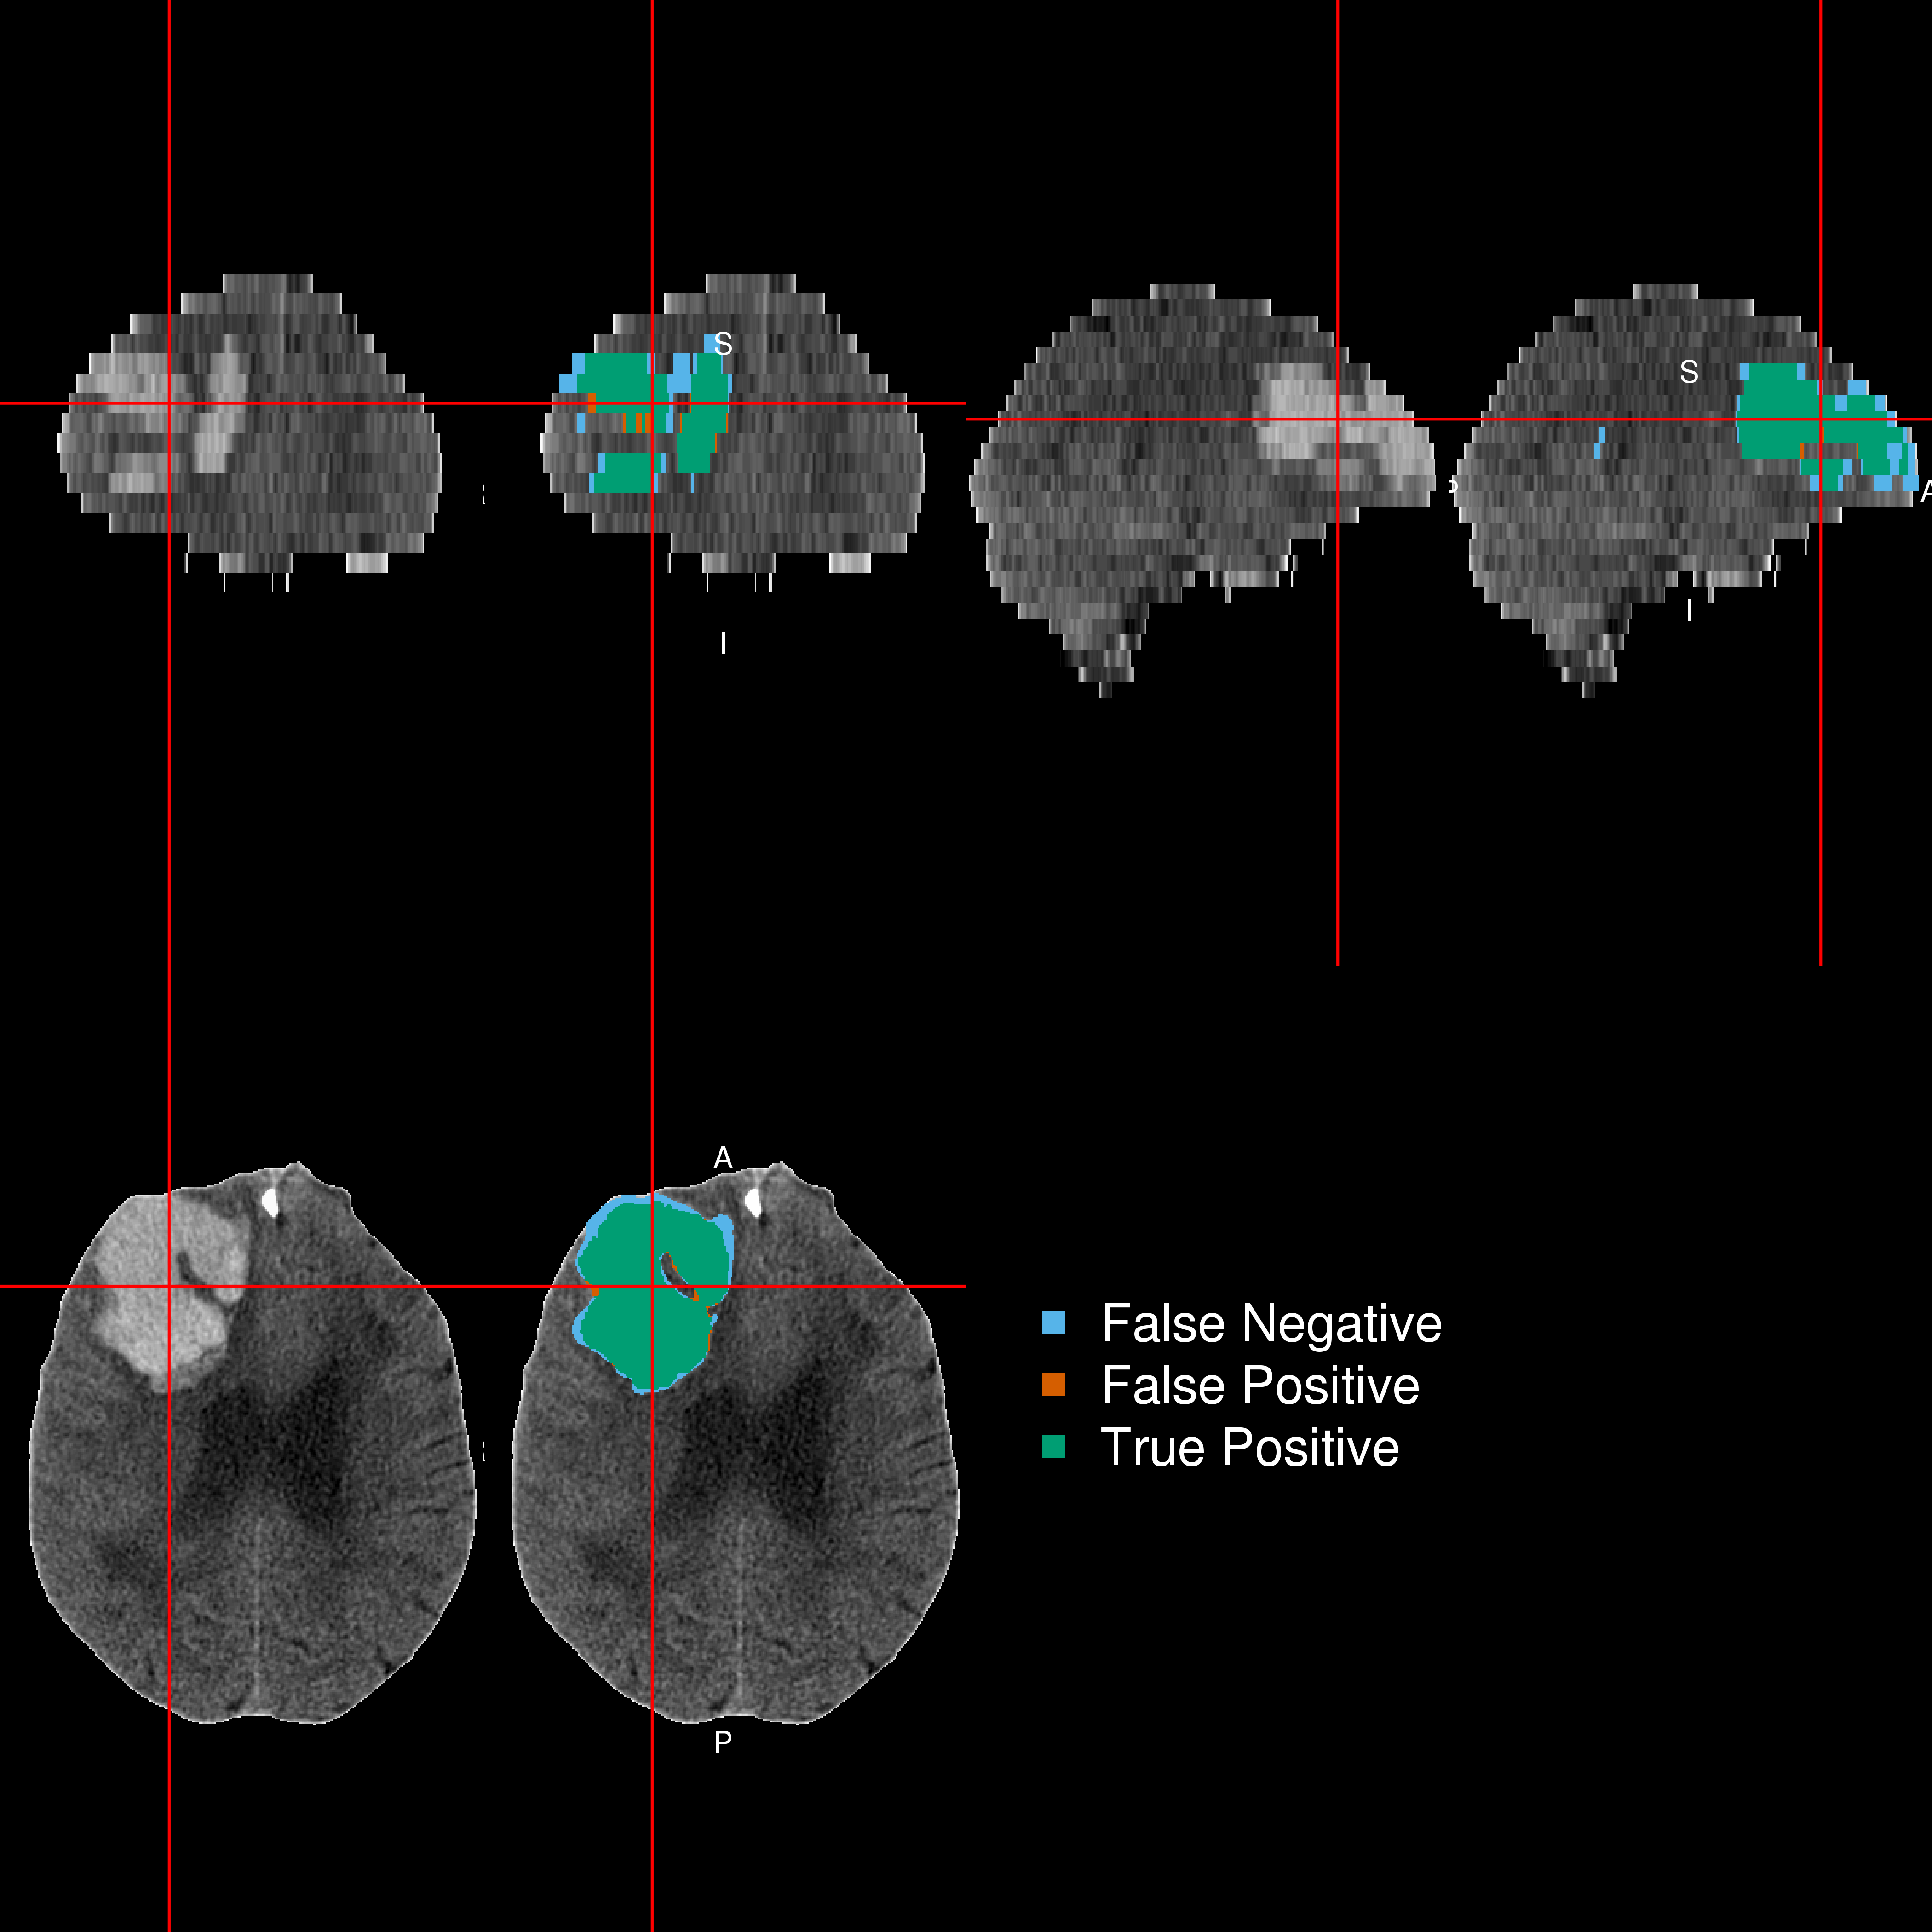
\includegraphics[width=0.75\linewidth,keepaspectratio]{Reseg_Figure_DSI_Quantile_025_native.png}
\caption{{\bf Patient with  25$^{\text{th}}$ Quantile Dice Similarity Index}. We present the patient with the 25$^{\text{th}}$ quantile Dice Similarity Index (DSI), a measure of spatial overlap, from the chosen predictor model fit with a random forest.  The 25$^{\text{th}}$ quantile DSI was 0.872. The green indicates a correct classification of ICH from the model, blue indicates a false negative, where the manual segmentation denoted the area to be ICH but the predicted one did not, and red indicates a false positive, where the predicted segmentation denoted the area to be ICH but the manual one did not. }
\label{fig:dice_img25}
\end{figure}

 \begin{figure}
\centering
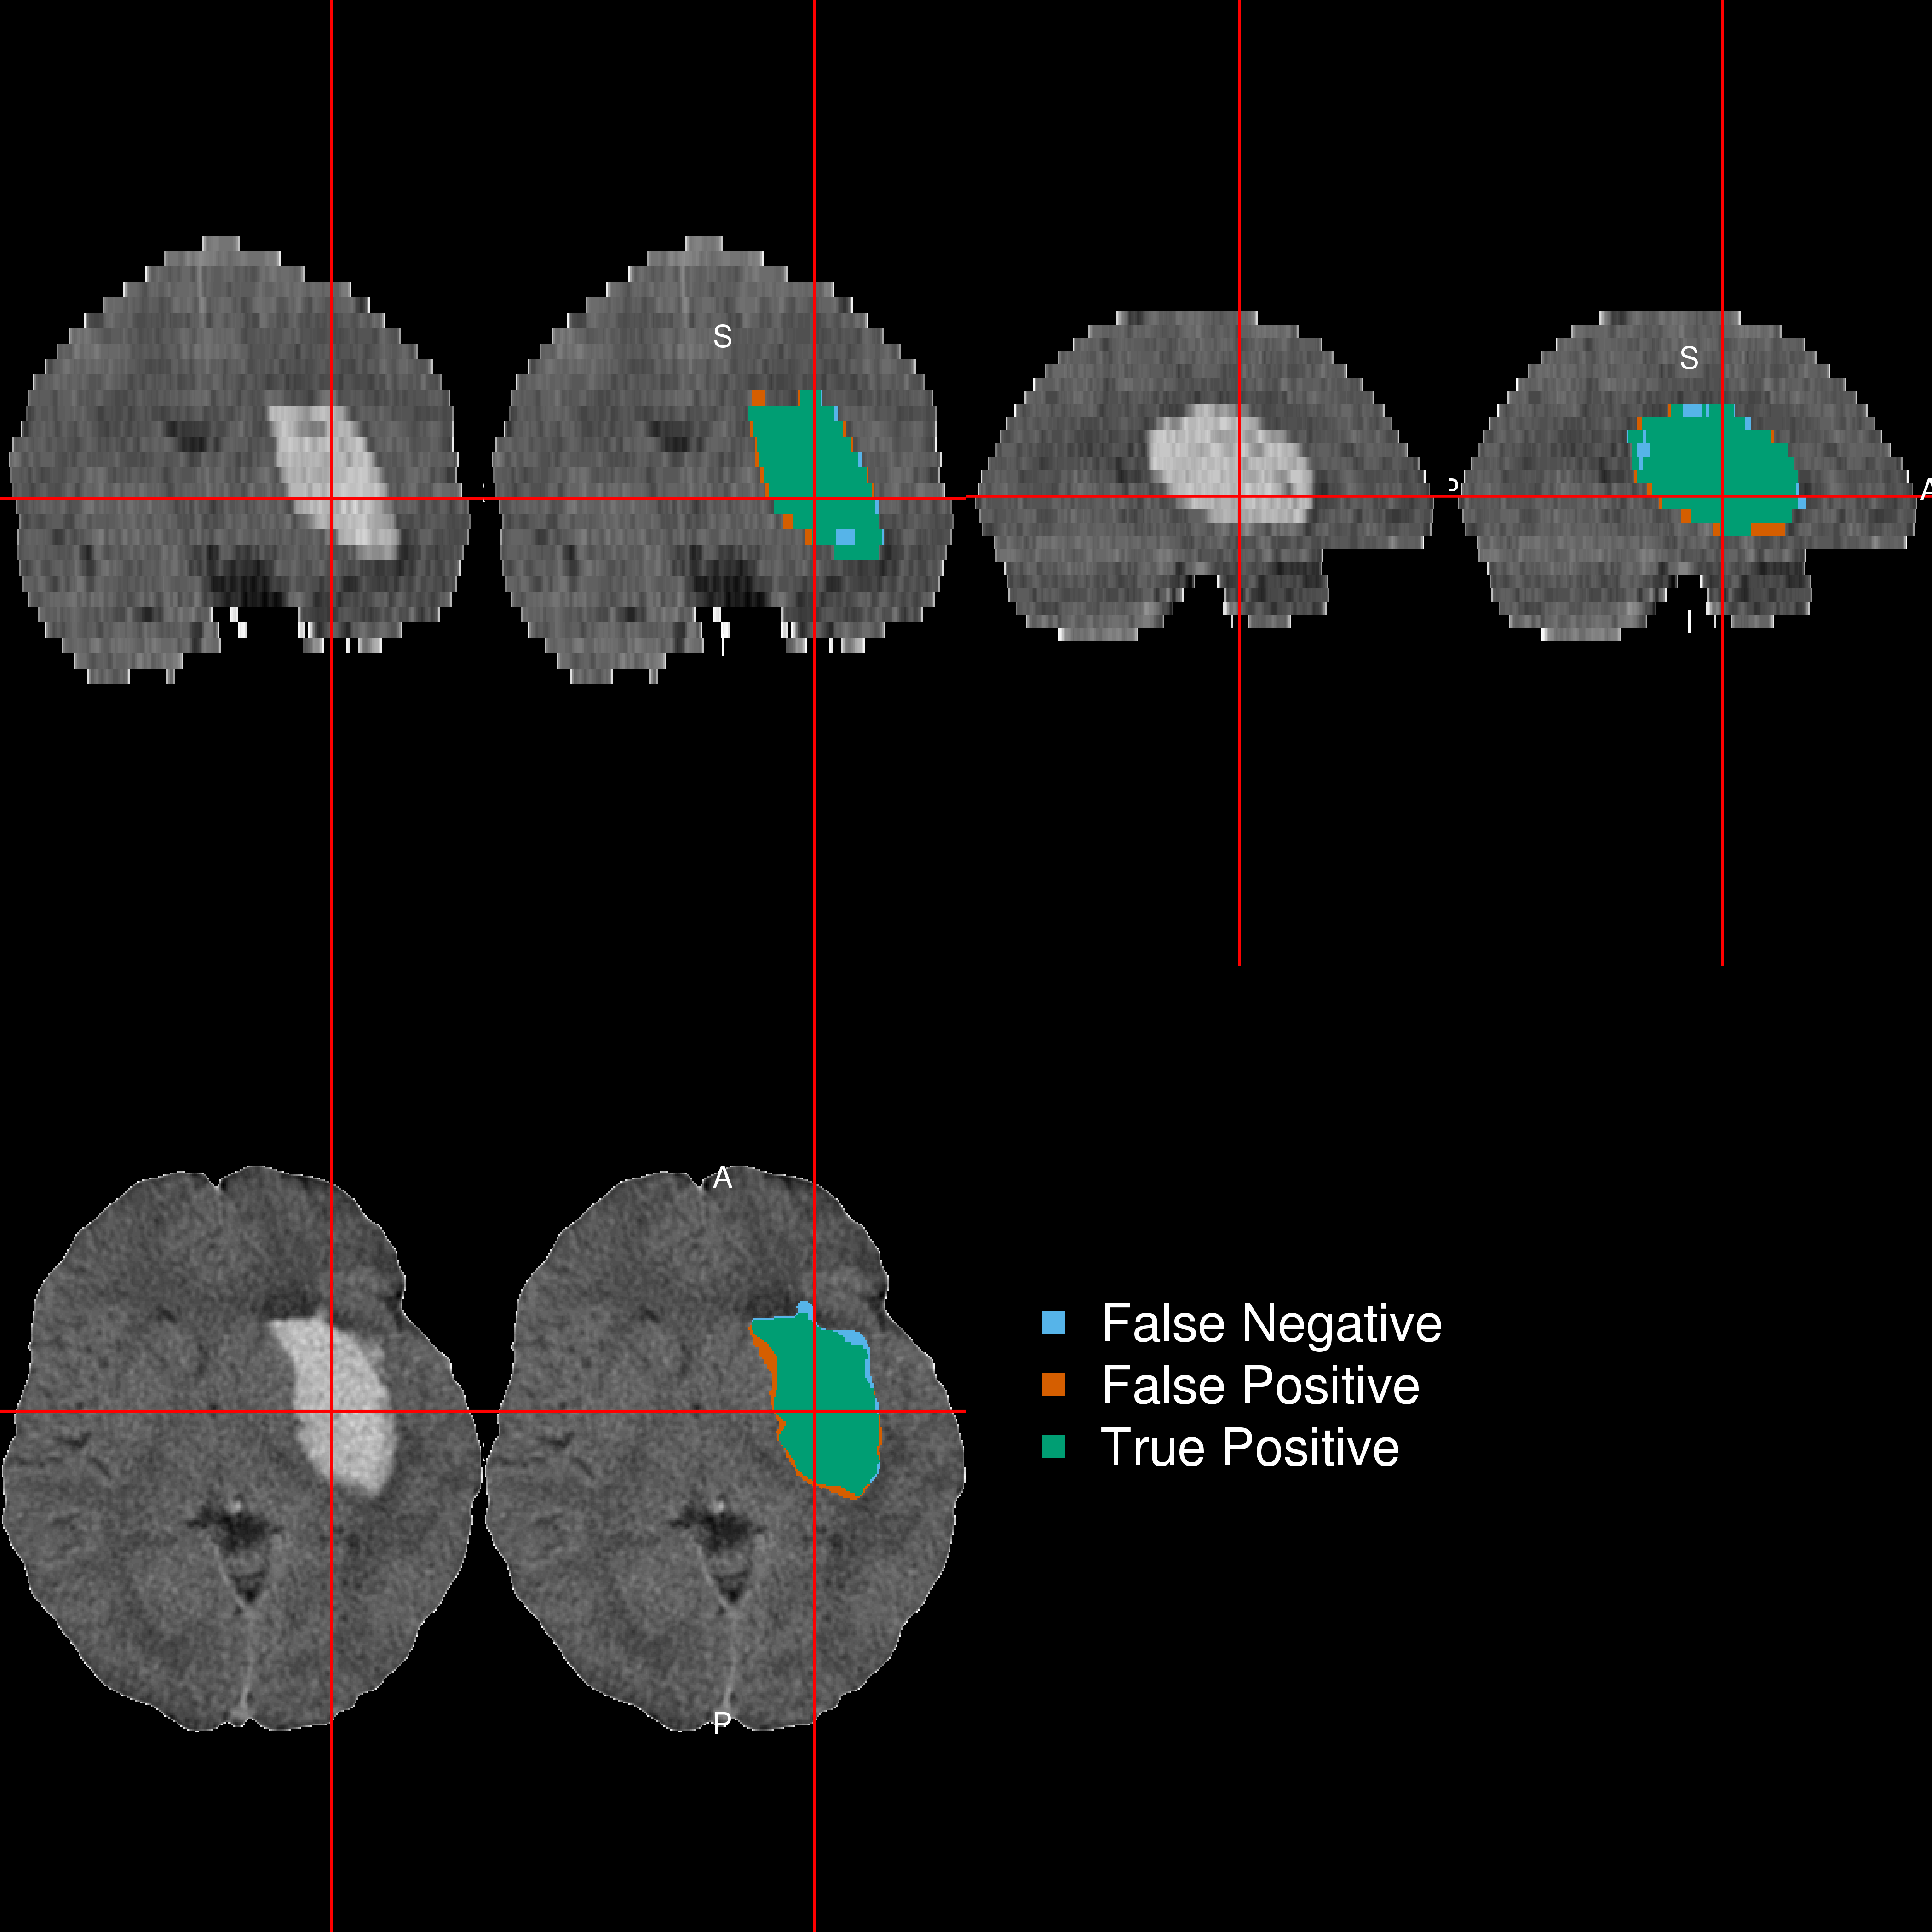
\includegraphics[width=0.75\linewidth,keepaspectratio]{Reseg_Figure_DSI_Quantile_075_native.png}
\caption{{\bf Patient with  75$^{\text{th}}$ Quantile Dice Similarity Index}. We present the patient with the 75$^{\text{th}}$ quantile Dice Similarity Index (DSI), a measure of spatial overlap, from the chosen predictor model fit with a random forest.  The 75$^{\text{th}}$ quantile DSI was 0.928. The green indicates a correct classification of ICH from the model, blue indicates a false negative, where the manual segmentation denoted the area to be ICH but the predicted one did not, and red indicates a false positive, where the predicted segmentation denoted the area to be ICH but the manual one did not. }
\label{fig:dice_img75}
\end{figure}

 \begin{figure}
\centering
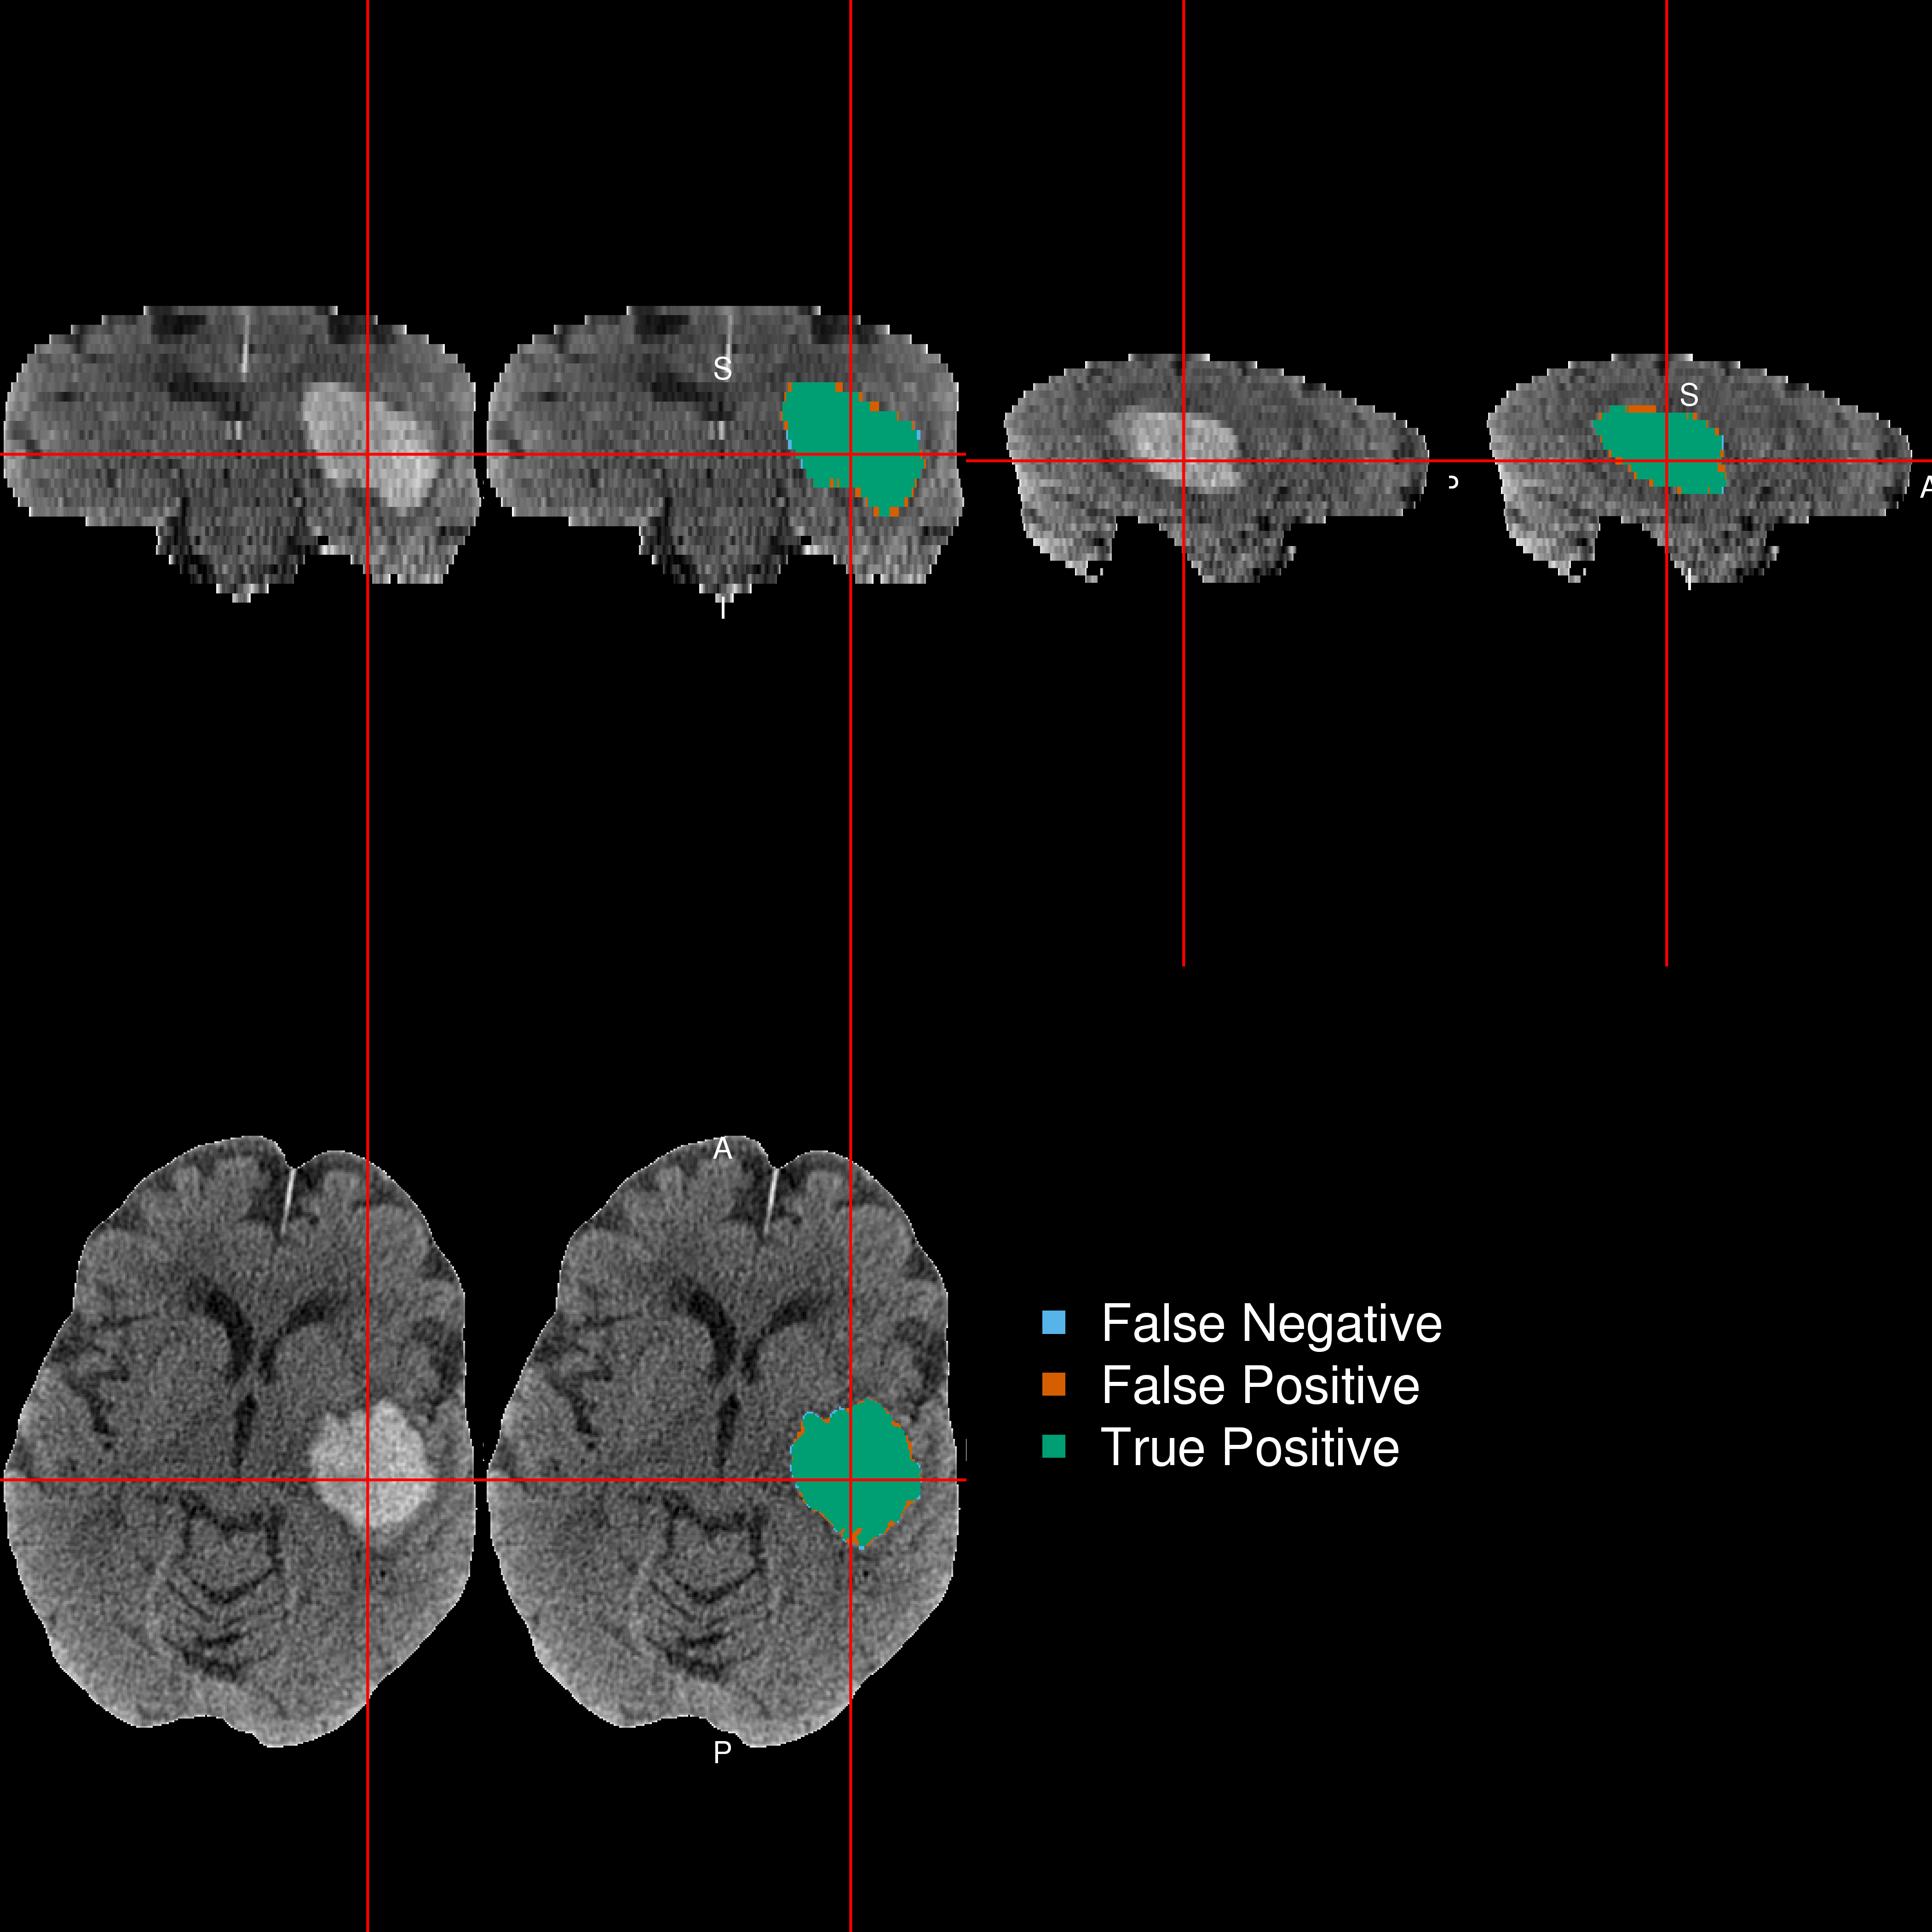
\includegraphics[width=0.75\linewidth,keepaspectratio]{Reseg_Figure_DSI_Quantile_100_native.png}
\caption{{\bf Patient with  Highest Dice Similarity Index}. We present the patient with the highest Dice Similarity Index (DSI), a measure of spatial overlap, from the chosen predictor model fit with a random forest.  The highest DSI was 0.956. The green indicates a correct classification of ICH from the model, blue indicates a false negative, where the manual segmentation denoted the area to be ICH but the predicted one did not, and red indicates a false positive, where the predicted segmentation denoted the area to be ICH but the manual one did not. }
\label{fig:dice_img100}
\end{figure}




\subsection{Model Specification}
\label{sec:modspec}

Let $Y_{i}(v)$ represent the binary hemorrhage mask indicator for voxel $v$, from patient $i$, and $x_{i,v}(k)$ represent the predictor image for image $k$, $k = 1, \dots 21$.
$$
\text{logit}\left(P(Y_{i}(v) = 1)\right) = \beta_0 + \sum_{k = 1}^{21} x_{i, k}(v)\beta_{k}
$$

The coefficients for the logistic model are (in log odds or log odds ratios):

% latex table generated in R 3.2.2 by xtable 1.8-0 package
% Fri Jan 29 01:30:54 2016
\begin{table}[ht]
\centering
\begin{tabular}{lr}
  \hline
Predictor & Beta \\ 
  \hline
Intercept & 1.008 \\ 
  Neighborhood mean & 0.051 \\ 
  Neighborhood sd & 0.000 \\ 
  Neighborhood skew & 0.065 \\ 
  Neighborhood kurtosis & -0.352 \\ 
  Image intensity (HU) & -0.172 \\ 
  Threshold ($>$= 40 and $<$= 80) & -0.151 \\ 
  Within-plane Coronal & -0.632 \\ 
  Within-plane Sagittal & -0.249 \\ 
  Within-plane Axial & 1.037 \\ 
  Winsorized standardized (20$\backslash$\% trim) & 0.547 \\ 
  Percentage thresholded neighbors & 2.061 \\ 
  Atropos probability image & 0.150 \\ 
  Percent of zero neighbors & -9.180 \\ 
  Indicator of any zero neighbors & 0.071 \\ 
  Distance to Image centroid & -0.087 \\ 
  Gaussian smooth (5mm\verb|^|3) & -0.051 \\ 
  Gaussian smooth (10mm\verb|^|3) & 0.550 \\ 
  Gaussian smooth (20mm\verb|^|3) & -0.390 \\ 
  Standardized-to-template Intensity & 1.460 \\ 
  Contralateral difference & 0.033 \\ 
   \hline
\end{tabular}
\end{table}


The specification for the functional form of the model fit with the LASSO penalty, is the same, but optimizes the following criteria:
$$
\min_{\beta} - \left( \frac{1}{\sum_{i}V_i} \sum_i Y_{i}(v) \times X_i(v)\beta - \log \left(1 + e^{X_i(v)\beta}\right) \right) +\lambda\sum_{k}\left|\beta_k\right|
$$






\cleardoublepage
\printbibliography[title={References}]
\end{refsection}

\begin{refsection}[stroke_chapter/stroke_chapter.bib]

































%\newpage 
%%\section{Title Page}
%\begin{flushleft}
%{\Large
%\textbf{Quantitative Localization of Supratentorial Intracranial Hemorrhage}
%}
%\\
%John Muschelli$^{1,\ast}$, ScM;
%Natalie L. Ullman$^{2}$, BS;
%Elizabeth M. Sweeney$^{1}$, ScM;
%Ani Eloyan$^{1}$, PhD; 
%Neil Martin$^{3}$, MD;
%Paul Vespa$^{3}$, MD;
%Daniel F. Hanley$^{2}$, MD;
%Ciprian M. Crainiceanu$^{1}$, PhD
%\\
%\bf{1} Department of Biostatistics, Bloomberg School of Public Health, Johns Hopkins University, Baltimore, MD
%\\
%\bf{2} Department of Neurology, Division of Brain Injury Outcomes,  Johns Hopkins Medical Institutions, Baltimore, MD
%\\
%\bf{3} Department of Neurosurgery, David Geffen School of Medicine at UCLA, Los Angeles, CA
%\\
%%\bf{4} Section of Neurosurgery and the Neurovascular Surgery Program, University of Chicago Pritzker School of Medicine, Chicago, IL
%%\\
%$\ast$ E-mail: jmusche1@jhu.edu
%\end{flushleft}
%

\newif\ifseverity
\severitytrue
\chapter{Quantitative Localization of Supratentorial Intracranial Hemorrhage}
\label{chap:stroke}


%% Please keep the abstract between 250 and 300 words
%\section{Abstract}
%
%
%\subsection{Background and Purpose}
%Standard radiologic description of intracranial hemorrhage (ICH) location is subjective and qualitative.  Using registration of computed tomography (CT) brain images, we provide objective, detailed quantification of ICH location.
%
%\subsection{Methods}
%We analyzed images from patients ($N{=}N$) enrolled in the MISTIE (Minimally Invasive Surgery plus recombinant-tissue plasminogen activator for Intracerebral Evacuation) trial.  We registered CT scans to a CT template, estimated a 3-dimensional map of ICH engagement location, and estimated areas of ICH engagement. 
%
%\subsection{Results}
%In this sample, ICH primarily located in deep brain nuclei and lobar white matter, including the insula, superior temporal gyrus, and the putamen.
%
%\subsection{Conclusions}
%Objective measures of ICH location and engagement using advanced CT imaging processing provide finer, objective, and more quantitative anatomic information than that provided by human readers. 
%
%\subsection{Clinical Trial Registration Information}
%Clinical Trial Registration-URL: \url{http://www.clinicaltrials.gov}. Unique identifier: NCT00224770.
%
%
%{\bf Keywords:} Intracerebral Hemorrhage; CT and MRI
%
%\newpage

\section{Introduction}

Intracranial hemorrhage (ICH) results from a blood vessel rupturing into brain tissues and possibly the ventricles. The classification and quantitative descriptions of hemorrhage location using X-ray computed tomography (CT) is complicated: it may extend into multiple brain areas, distend tissues, and break through the ventricular wall. Therefore, routine practice identifies one primary affected anatomic region (e.g.~caudate) \citep{mendelow_early_2013, anderson_intensive_2008, antihypertensive_treatment_of_acute_cerebral_hemorrhage_atach_investigators_antihypertensive_2010} or describes the hemorrhage in relation to a landmark \citep{ziai_multicenter_2014}.

Detailed localization information can be obtained, however, by registering scans to a common template where labeled brain atlases are available. After registration, each patient scan is located in the same stereotaxic template space so information may be combined spatially across scans. We registered CT images to a previously-published CT template \citep{rorden_age-specific_2012}, located in MNI (Montreal Neurological Institute) space, using the provided software. 

Our goal is to quantitatively and objectively characterize ICH location\ifseverity
, compare this characterization to human labeling, and predict stroke severity scores using ICH location information. 
\else
.
\fi


\section{Methods}

To achieve this goal, we 1) created a 3-dimensional (3D) density map of supratentorial hemorrhages\ifseverity
, 
\else
 and 
\fi 2) provided detailed quantification of hemorrhage engagement of individual neuroanatomic regions\ifseverity
, 3) performed voxel-wise tests of ICH location on 2 severity scores: Glasgow Coma Scale (GCS) and National Institutes of Health Stroke Scale (NIHSS) and 4) summarized significantly predictive voxel regions into patient-level covariates.
\else 
.
\fi



\subsection{Subjects and Demographics}
The population studied consists of 111 patients from the MISTIE (Minimally Invasive Surgery plus recombinant-tissue plasminogen activator for Intracerebral Evacuation) \citep{morgan_preliminary_2008} trial recruited from 26 centers with lobar and deep ICHs $\geq$20mL in volume.    This sample was $31.5$\% female with mean (SD) age of 60.8 (11.2) years.

% Descriptive demographics of age, sex, race, and baseline ICH and intraventricular hemorrhage (IVH) volumes are shown in Table~\ref{t:dem}.  

% CT and clinical data were collected as part of the Johns Hopkins Medicine IRB-approved MISTIE research studies with written consent from participants. 

\thickmuskip=0mu

\subsection{Imaging Data}
Standard diagnostic CT images were acquired under a standard protocol but with differences across sites.  Scans were acquired using GE ($N{=}46$), Siemens ($N{=}37$), Philips ($N{=}20$), and Toshiba ($N{=}8$) scanners, had gantry tilt ($N{=}87$), and the slice thickness of the image varied within some scans ($N{=}14$). Therefore, the scans analyzed had different voxel (volume element) dimensions and image resolution prior to registration to the template. 
%These conditions represent a pragmatic sample of stroke center diagnostic imaging.
\thickmuskip=5mu plus 5mu


\subsection{Hemorrhage Segmentation and Location Identification}
ICH was manually segmented using the OsiriX (v.4.1, Pixmeo; Geneva, Switzerland) by expert readers.  Readers employed a semi-automated approach: a Hounsfield unit range of $40$ to $80$ selected potential regions of ICH \citep{bergstrom_variation_1977, smith_imaging_2006}, then these regions were manually adjusted. Readers identified the anatomic location most engaged by the ICH: putamen ($N{=}68$), lobar ($N{=}33$), globus pallidus ($N{=}6$), and thalamus ($N{=}4$).  The initial mean (SD) ICH volume of this sample was 37.4 (20.1) mL.


\subsection{Image Registration}
The brain image was spatially registered to the CT template using the Clinical toolbox \citep{rorden_age-specific_2012} and the statistical parametric mapping software (SPM8, Wellcome Trust Centre for Neuroimaging, London, UK) in MATLAB (Mathworks, Natick, Massachusetts, USA).  The binary hemorrhage mask was transformed into the template space. No scans were excluded due to inadequate registration, determined by visual inspection.


\subsection{ICH Localization and Engagement}
\label{sec:engage}
We estimated a 3D histogram of ICH localization: for every voxel in template space, we calculated the proportion of patients who have an ICH at that particular voxel.  
 
%Although prediction of severity score is of interest, standard practice conveys information based on known neuroanatomic regions.  
We calculated spatial ICH engagement by neuroanatomic region using the ``Eve" atlas \citep{oishi_human_2008}, which segments gray matter (GM) and white matter (WM) regions.  
Ventricular regions were not explicitly segmented in the Eve atlas.  Any region not classified was reported as cerebrospinal fluid (CSF).


From this atlas, we estimated ICH engagement at the population level: 1) the percent of the ICH engaged by region (e.g.~putamen engages 20\% of the ICH) and 2) the percent of each region engaged by the ICH (e.g.~ICH engages 78\% of the putamen).  These summaries of ICH engagement provide a finer description than one location (e.g.~putamen).  

\ifseverity
In the study population, 1,045,174 voxels (denoted by $V$) had at least one patient with ICH.  We limited our analysis to voxels in the template space where at least 10 patients exhibit ICH (166,202 voxels) to optimize the models for a substantial proportion of the study population.

We tested the association between hemorrhage location and stroke severity by running voxel-wise t-tests, testing the null hypothesis $H_{0}(v):\mu_{1}(v)=\mu_{0}(v)$, where $\mu_{1}(v)$ corresponds to the mean score (NIHSS or GCS) in patients where $ICH{=}1$ at voxel $v$, similarly for $\mu_{0}(v)$. 


We created a patient-level covariate that summarizes ICH location information by selecting regions using a sequence of nested p-value thresholds.  We call these regions ``highest predictive regions'' (HPR) because they contain the voxels that are most predictive of the severity scores. 
We obtained $6$ different HPR, $3$ based on the smallest $1000$, $2000$, or $3000$ lowest p-values and three based on p-values thresholds of $.05$, $.01$, and $.001$. For each HPR, we calculated the HPR ``coverage" for scan $i$: 
$$
\text{HPR Coverage}_i = \frac{\text{\# Voxels classified ICH in HPR for scan } i}{\text{\# Voxels in HPR}} \times 100\% \nonumber
$$
and used this as a predictor of the severity score ($Y_i$), adjusting for age, sex, and baseline ICH volume (ICHVol):
\begin{equation}
{\rm Y}_i = \beta_0 + \beta_1 {\rm Coverage}_i + \gamma_1{\rm Age}_i  +\gamma_2{\rm Sex}_i +\gamma_3{\rm ICHVol}_i + \epsilon_{i} \label{eq:cov}
\end{equation}
\thickmuskip=0mu
We compared model~\eqref{eq:cov} using adjusted $R^2$ to one using a categorical indicator of the expert-specified ICH location, with categories: thalamus, globus pallidus, putamen, and lobar.  
A permutation test was used: the severity score was randomly permuted, the HPR was estimated, and the adjusted $R^2$ was calculated. The p-value was obtained by comparing the distribution of permuted adjusted $R^2$ with the estimated adjusted $R^2$ from the HPR model. 
\fi
\section{Results}

\subsection{Prevalence of ICH Engagement in the Brain}

Figure~\ref{fig:StrokeHist} represents the 3D histogram of hemorrhage prevalence, where colors represent the percentage of patients with ICH engagement at that voxel.  ICH is distributed medially in the brain in this cohort, with a lower concentration at the cortical surface and higher on the left side of the brain.   The majority of voxels have a low prevalence of ICH engagement; the median number of patients with ICH at a voxel is 3 (3\%), though some voxels ($V{=}5685$) have a high prevalence of ${>}40\%$ of the sample population.  


\thickmuskip=5mu plus 5mu

%***
%Combining regions of engagement from the left and right sides of the brain is worthwhile as regions will likely affect severity regardless of the hemisphere engaged. We did not combine these areas, as it may not be straightforward to combine ICH that crosses the mid-sagittal plane. We did attempt to ``symmetrize'' the HPR by including voxels regardless of the side of the brain.  If a voxel on the left side of the brain was included in the HPR, the corresponding voxel on the right side was included in the symmetrized HPR.  We observed similar patterns to Figure 3C and 3D using the symmetrized HPR  (see \url{http://stroke.ahajournals.org}).


\subsubsection{ICH Localization and Engagement}
Table~\ref{t:breakdown} represents the 10 most-engaged regions for the population 3D histogram.  The engagement represents the percent engagement of a specific area compared to all areas engaged.  The 3D histogram of ICH is engaged in areas of the insula, putamen, and primarily the CSF (i.e.~ventricles and subarachnoid spaces). 

We also calculated the engagement of the thalamus, putamen, and globus pallidus by the population 3D histogram.  The population engagement represents the mean proportion of ICH prevalence in the population for that brain region.  On average, 23\% of the putamen, 20\% of the globus pallidus, and 8\% of the thalamus are engaged with ICH from patients in this study. 

Registering images with large deformations caused by the hemorrhage, even those using non-linear registration, will likely have mis-registration artifacts.  Lateral shift caused by the hemorrhage, resulting in compression of ventricles, may lead to mapping some areas of the hemorrhage or tissue to the ventricles in template space.  Combining multiple registration approaches may achieve better results.



\ifseverity
\subsubsection{Highest Predictive Region Analysis}




\thinmuskip=0mu


For illustration, panel (\protect\subref*{pvals:nihss}) in Figure~\ref{f:roi} displays the region of p-values smaller than $.01$ for the voxel-wise t-tests of NIHSS and panel~(\protect\subref*{pvals:gcs}) displays voxels with the smallest $1000$ p-values testing GCS score. These regions were the HPR with the highest adjusted $R^2$ in \eqref{eq:cov}. We show three orthographic slices for each HPR; the entire regions are available in MNI coordinates. 
\thinmuskip=3mu

Figure~\ref{f:roi}\protect\subref*{pvals:regnihss} displays the NIHSS score as a function of the coverage of the HPR from Figure~\ref{f:roi}\protect\subref*{pvals:nihss}. Similarly, Figure~\ref{f:roi}\protect\subref*{pvals:reggcs} displays the GCS score as a function of the coverage of the HPR in Figure~\ref{f:roi}\protect\subref*{pvals:gcs}.  The blue line represents a non-parametric LOESS (local regression) \citep{cleveland_local_1992} fit and the red line represents an unadjusted linear model fit.  As expected, the larger the HPR coverage the higher (more severe stroke) the NIHSS score and the lower (deeper unconsciousness) the GCS score.

Adjusted $R^2$ model estimates indicated all HPR coverage models strongly outperform reader-classified location models: the adjusted $R^2$ almost doubled from $0.129$  for the reader-classified location model to $0.254$ for NIHSS; the adjusted $R^2$ more than tripled from $0.069$ for the reader-classified location model to $0.214$ for the HPR coverage model for GCS. 

The permutation test p-values were $<.001$ for HPR of NIHSS and $<.01$ for HPR of GCS, indicating that the selected HPRs were more predictive than HPRs obtained using the same selection procedure when there is no association between location and stroke severity scores. 
\fi

\section{Discussion}

We have characterized the localization of ICH in a population from prospective clinical trial images using a 3D histogram. We found the well-described medial location of most supratentorial ICHs.   We can create 3D histograms based on subgroups or different study populations and test differences between groups at a voxel level using proportion tests, allowing a fine-scale comparison ICH location across groups.

We also demonstrate how labeled atlases can automatically describe ICH engagement by neuroanatomic regions at a patient or population level. These measures are more interpretable for clinical relevance and may translate to better determination of disability.


\subsection{Summary}
The summary of Eve-atlas ICH engagement presented provided a finer description of location than previously possible by human readers. This type of analysis provides a framework for derivation and testing measures of ICH engagement.  We hope this method will engage others with larger data sets and methodological skills to enhance the use of quantitative localization. 



\section{Sources of Funding}
The project described was supported by the grant RO1EB012547 (NIH), T32AG000247 (NIA), R01NS046309, RO1NS060910, RO1NS085211, R01NS046309, U01NS080824 and U01NS062851 (NINDS), and RO1MH095836 (NIMH).

\section{Disclosures}
Johns Hopkins University holds a use patent for intraventricular tissue plasminogen activator.



% \section{Acknowledgments}


%\clearpage
%\newpage
%\thispagestyle{empty}
%\pagestyle{plain}
%
%% \bibliographystyle{plainnat}
%% \bibliography{CT_Pipeline}
%\defbibheading{myheading}[References]{%
%  \section{#1}}
%\printbibliography[heading=myheading]
  
%\printbibliography[title=References]




\clearpage
\newpage
\thispagestyle{empty}
\pagestyle{plain}


\section{Tables}


%% latex table generated in R 3.2.2 by xtable 1.8-0 package
% Fri Jan 29 01:56:29 2016
\begin{table}[ht]
\centering
\begin{tabular}{lc}
  \hline { Variable (N=111)} & { N (\%) or Mean (SD)} \\ 
  \hline
Age in Years: Mean (SD) & 60.8 (11.2) \\ 
   \hline
Female & 35 (31.5\%) \\ 
   \hline
ICH Volume: Mean (SD) & 37.4 (20.1) \\ 
   \hline
IVH Volume: Mean (SD) & 3.2 (6.3) \\ 
   \hline
Reader-Classified ICH Location &  \\ 
   \hline
\text{  } Putamen & 68 (61.3\%) \\ 
   \hline
\text{  } Lobar & 33 (29.7\%) \\ 
   \hline
\text{  } Globus Pallidus & 6 (5.4\%) \\ 
   \hline
\text{  } Thalamus & 4 (3.6\%) \\ 
   \hline
\end{tabular}
\caption{} 
\label{t:dem}
\end{table}








%% latex table generated in R 3.2.2 by xtable 1.8-0 package
% Fri Jan 29 01:56:30 2016
\begin{table}[ht]
\centering
\begin{tabular}{lccc}
  \hline
Area & Population Prevalence & NIHSS HPR & GCS HPR \\ 
  \hline
CSF (ventricular \& subarachnoid spaces) & 7.9 & 10.0 & 4.2 \\ 
  Insula & 4.7 &  &  \\ 
  Superior temporal gyrus & 3.8 &  &  \\ 
  Putamen left & 3.0 &  &  \\ 
  Insular right & 2.9 &  &  \\ 
  External capsule left & 2.3 &  &  \\ 
  Superior corona radiata left & 1.9 & 11.8 & 27.9 \\ 
  Superior temporal wm left & 1.9 &  &  \\ 
  Superior corona radiata right & 1.8 &  &  \\ 
  Putamen right & 1.8 &  &  \\ 
  Posterior limb of internal capsule left &  & 10.1 & 3.9 \\ 
  Thalamus left &  & 7.6 & 33.9 \\ 
  Caudate nucleus left &  & 5.4 & 9.6 \\ 
  Superior longitudinal fasciculus left &  & 4.9 & 5.9 \\ 
  Globus pallidus left &  & 3.7 &  \\ 
  Anterior limb of internal capsule left &  & 3.6 &  \\ 
  Outside brain mask &  & 3.5 &  \\ 
  Anterior limb of internal capsule right &  & 3.0 &  \\ 
  Postcentral wm left &  &  & 6.7 \\ 
  Posterior corona radiata left &  &  & 3.1 \\ 
  Precentral wm left &  &  & 1.3 \\ 
  Supramarginal wm left &  &  & 1.1 \\ 
   \hline
\end{tabular}
\caption{Percent engagement of the 3D histogram and top-performing HPR for the top 10 areas of engagement} 
\label{t:breakdown}
\end{table}

% latex table generated in R 3.2.2 by xtable 1.8-0 package
% Fri Jan 29 01:56:31 2016
\begin{table}[ht]
\centering
\begin{tabular}{lc}
  \hline
Area & Population Prevalence \\ 
  \hline
CSF (ventricular \& subarachnoid spaces) & 7.9 \\ 
  Insular & 7.6 \\ 
  Superior temporal gyrus & 5.5 \\ 
  Putamen & 4.8 \\ 
  External capsule & 3.9 \\ 
  Superior corona radiata & 3.7 \\ 
  Precentral gyrus & 3.3 \\ 
  Precentral WM & 3.1 \\ 
  Superior temporal WM & 3.1 \\ 
  Posterior limb of internal capsule & 3.0 \\ 
   \hline
\end{tabular}
\caption{{\bf Distribution of the Top 10 Areas of Engagement of Highest Predictive Regions.}} 
\label{t:breakdown}
\end{table}





\clearpage
\newpage

\section{Figures}

\setcounter{figure}{0}


\begin{figure}[H]
\centering
  \subfloat{
  \label{prop:img}	
	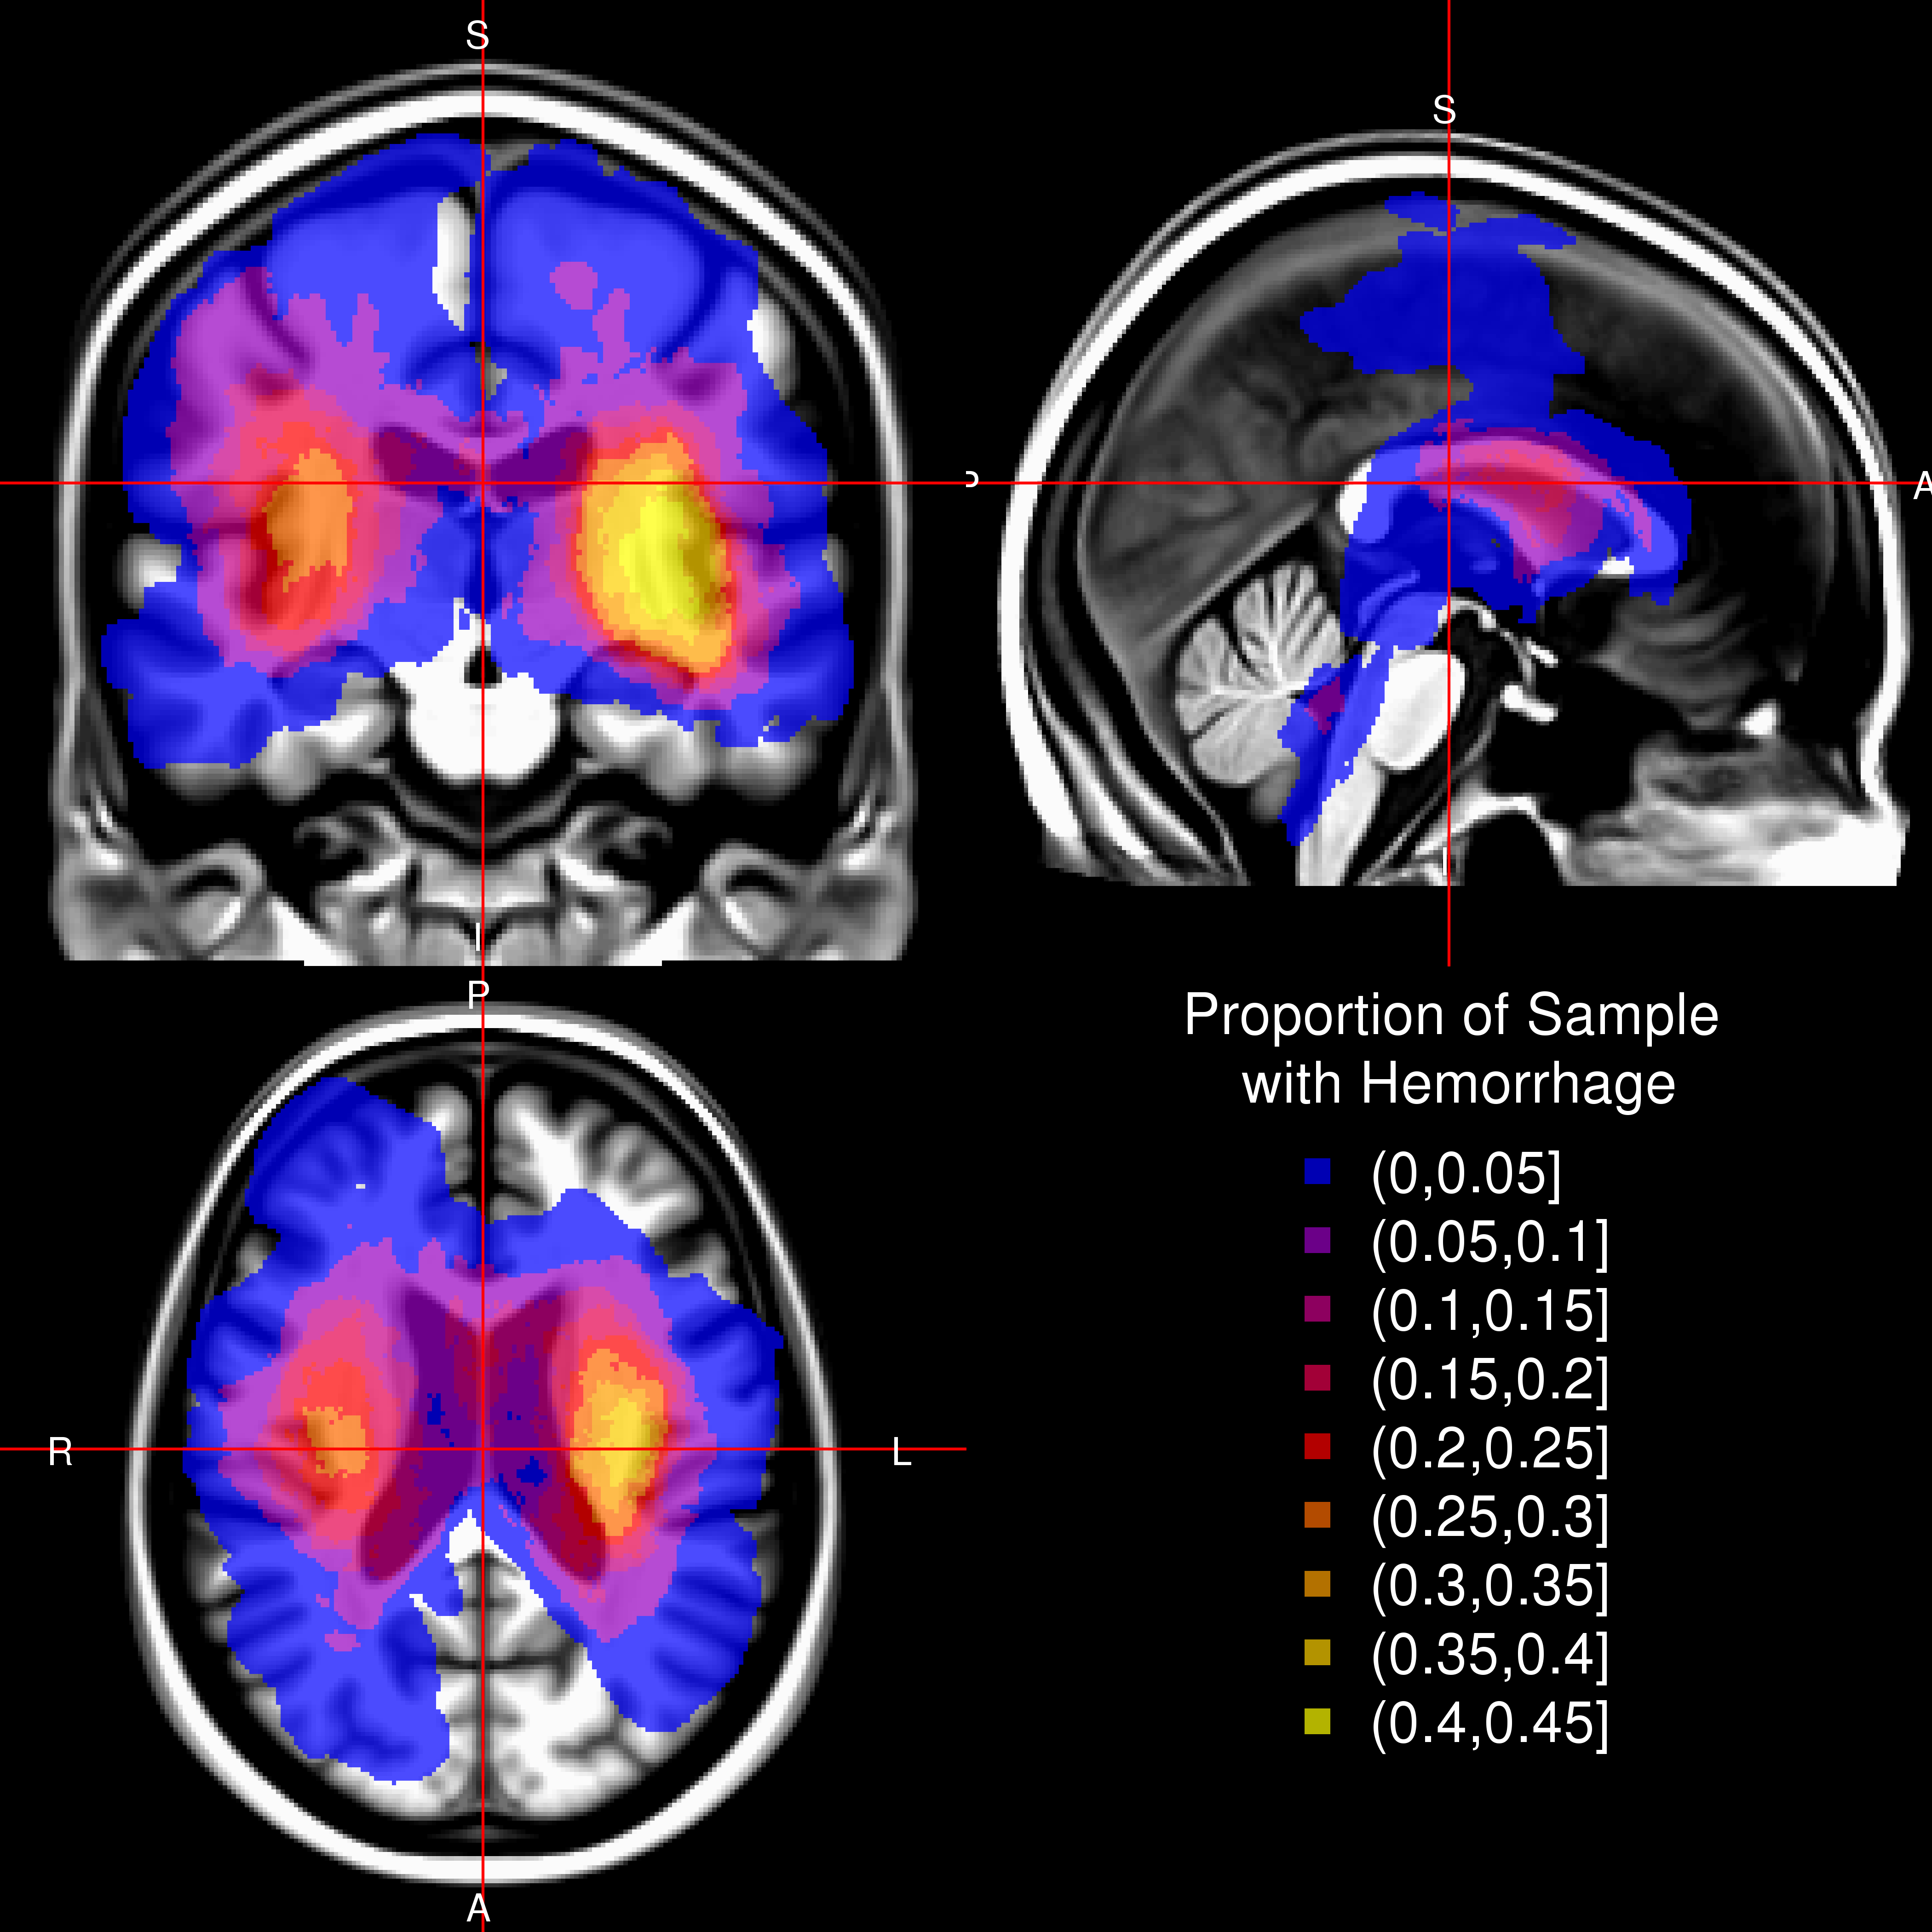
\includegraphics[width=.98\textwidth]{Figure4_Proportion_Final.png}
}
\caption[{\bf ICH Engagement Prevalence.}]{{\bf ICH Engagement Prevalence.} The proportion of patients with ICH engaging a given voxel are represented in a 3D histogram (right side of image is left side of brain) overlaid on an MRI T1 template. There is a higher prevalence of ICH on the left side of the brain, localized in the middle of the brain, with few extensions in the anterior and posterior areas. The interactive version of this figure is located at \url{http://muschellij2.github.io/CT_Pipeline/index.html}.}
  \label{fig:StrokeHist}
\end{figure}



\ifseverity
\begin{figure}[H]
\centering
  \hfill
  \subfloat{
 \label{pvals:nihss}
 \includegraphics[width=.48\textwidth]{{Top_0.01_pvalues_Final}.png}
 }
  \hfill
  \subfloat{
 \label{pvals:gcs} 
 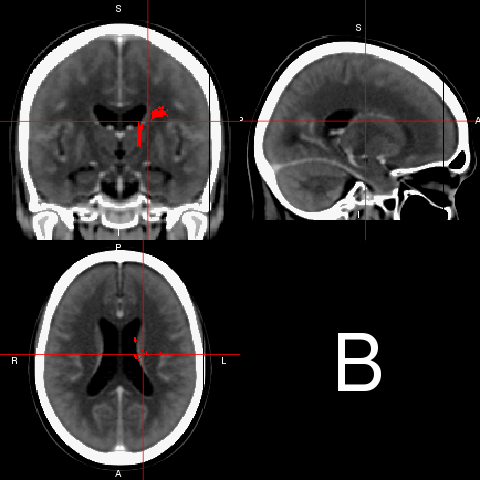
\includegraphics[width=.48\textwidth]{GCS_Top_1000_pvalues_Final.png}
 } 
 \newline
  \hfill
  \subfloat{
 \label{pvals:regnihss}
 \includegraphics[width=.48\textwidth]{Regress_ROI_NIHSS_Best_Model.png}
 }
  \hfill
  \subfloat{
 \label{pvals:reggcs}
 \includegraphics[width=.48\textwidth]{Regress_ROI_GCS_Best_Model.png}
 }  
  \caption[{\bf Highest Predictive Region (HPR) Analysis.}]{{\bf Highest Predictive Region (HPR) Analysis.}  Panels~\protect\subref{pvals:nihss} and~\protect\subref{pvals:gcs} correspond to the HPR for the top-performing model for NIHSS and GCS scores.  The HPR in \protect\subref{pvals:nihss} represents a p-value threshold of $.0100$ ($19047$ voxels) for the voxel-wise p-value of ICH on NIHSS. The HPR in \protect\subref{pvals:gcs} represents $1000$ with the lowest p-values for the voxel-wise ICH on GCS score regressions.
    Panels~\protect\subref{pvals:regnihss} and~\protect\subref{pvals:reggcs} plot the relationship of the HPR coverage and severity score.  The red line represents a linear fit, the blue line--a LOESS fit.  The larger the HPR coverage the higher (more severe) the NIHSS and the lower (deeper unconsciousness) the GCS.
}
  \label{f:roi}
\end{figure}
\fi



%
%\clearpage
%\newpage
%
%\thispagestyle{empty}
%\pagestyle{plain}
%
%\setcounter{figure}{0}
%\renewcommand{\thefigure}{\Roman{figure}}
%\setcounter{table}{0}
%\renewcommand{\thetable}{\Roman{table}}


\cleardoublepage
\printbibliography[title={References}]
\end{refsection}

\begin{refsection}[ss_chapter/ss_chapter.bib]
















\chapter{Validated Automatic Brain Extraction of Head CT Images}
\label{chap:ss}


\section{Introduction}

X-ray computed tomography (CT) scanning of the brain is widely available and is a commonly used diagnostic tool in clinical settings \citep{sahni_management_2007, chalela2007magnetic, schellinger1999standardized}. Though analysis of CT images is typically done by qualitative visual inspection, detailed quantification of information using neuroimaging tools is of interest.  The reason for this interest is that qualitative inspection of CT scans provides limited quantifiable information that can be used in research. A fundamental processing step for producing quantifiable and  reproducible information about the brain is to extract the brain from the CT image. This process is called brain extraction or skull stripping.  This step is necessary because CT images contain non-brain human tissues and non-human elements (e.g. pillow, medical devices) that are not pertinent to brain research.  We propose a validated automated solution to brain extraction in head CT scans using established neuroimaging software.

In magnetic resonance imaging (MRI), brain extraction has been extensively studied and investigated (see \citet{wang2014knowledge} for an overview of methods).  While an extensive literature accompanied by software exist for brain MRI scans, the same is not true for brain CT scans.  \citet{smith_fast_2002} introduced and validated the Brain Extraction Tool (BET), a function of the FSL \citep{jenkinson_fsl_2012} neuroimaging software (v5.0.4), to automatically extract the brain from MRI scans.  Here we propose to adapt BET and validate its brain extraction performance for CT scans.  

BET adaptations for this purpose have been presented before in \citet{solomon_user-friendly_2007}.  Although the method is similar to that outlined below, using thresholding and then applying BET, the authors did not publish the specific details of the method nor any code to evaluate it.  To replicate the method from \citet{solomon_user-friendly_2007}, \citet{rorden_age-specific_2012} thresholded voxels to be under 100 Hounsfield units, manually adjusted the image intensity to enhance the soft tissue in the brain, and then BET was applied with a fractional intensity of $0.35$.  Therefore, brain extraction methods from \citet{rorden_age-specific_2012} and \citet{solomon_user-friendly_2007} strongly parallels the proposed method described below, but neither studies presented a formal validation against a set of manually segmented brain images.  

\citet{mandell2014volumetric1} has recently proposed a brain extraction method for CT scans and has done a validation against manual segmentation.  This method was also performed on a set of brains with disease \citep{mandell2014volumetric2, mandell2014volumetric3}.  This method is not fully automated, however.   \citet{mandell2014volumetric1} has formally validated a brain extraction method against manually segmented images, but the method requires user interaction.  

Thus, the goals of our study are to propose an automated method that has been formally validated against a set of manually segmented images and estimate brain extraction performance of this method in a large number of CT scans.





\section{Methods}
\subsection{ Participants and CT data}
We used CT images from patients enrolled in the MISTIE (Minimally Invasive Surgery plus recombinant-tissue plasminogen activator for Intracerebral Evacuation) and ICES (Intraoperative CT-Guided Endoscopic Surgery) stroke trials \citep{morgan_preliminary_2008}.  Inclusion criteria into the study included: $18$ to $80$ years of age, spontaneous supratentorial intracerebral hemorrhage above $20$ milliliters (mL) in size (for full criteria, see \citet{mould_minimally_2013}).  The population analyzed here had a mean (SD) age was $60.6$ $(11.6)$ years, was $66.9\%$ male, and was 55.6\% Caucasian, 30.1\% African American, 9.8\% Hispanic, and 4.5\% Asian or Pacific islander.  CT data were collected as part of the Johns Hopkins Medicine IRB-approved MISTIE research studies with written consent from participants.  


\subsection{Imaging Data}
\subsubsection{Validation of Automated Head Segmentation}
For the validation of automated segmentation against gold standard manual segmentation, we analyzed 36 scans, corresponding to 36 unique patients.  The study protocol was executed with minor, but important, differences across the 19 sites.  Scans were acquired using Siemens ($N=14$), GE ($N=11$), Philips ($N=10$), and Toshiba ($N=1$) scanners. Gantry tilt was observed in 21 scans.  Slice thickness of the image varied within the scan for 7 scans. For example, a scan may have 10 millimeter (mm) slices at the top and bottom of the brain and 5mm slices in the middle of the brain.  Therefore, the scans analyzed had different voxel (volume element) dimensions and image resolution prior to registration to the template.  These conditions represent how scans are presented for evaluation in many diagnostic cases.  

%n_crani_problem 
%n_gantry_problem 


\subsection{Manual and Automated Brain Extraction}
Brain tissue was manually segmented as a binary mask from DICOM (Digital Imaging and Communications in Medicine) images using the OsiriX imaging software (OsiriX v.4.1, Pixmeo; Geneva, Switzerland) by one expert reader (reader 1: NU). 
CT brain images and the binary brain tissue mask obtained using manual segmentation were exported from OsiriX to DICOM format.  

\subsection{Image Processing}
The image processing pipeline is provided in Figure~\ref{fig:framework}.
Images with gantry tilt were corrected using a customized MATLAB (The Mathworks, Natick, Massachusetts, USA) user-written script (\url{http://bit.ly/1ltIM8c}).  Although gantry tilt correction is not inherently necessary for brain extraction, it is required for rigid co-registration of scans within a patient, which is a common processing step in longitudinal analysis of images post brain extraction. 

Images were converted to the Neuroimaging Informatics Technology Initiative (NIfTI) data format using \texttt{dcm2nii} (2009 version, provided with MRIcro \citep{rorden_stereotaxic_2000}).  Images were constrained to values between $-1024$ and $3071$ HU to remove potential image rescaling errors and artifacts.  No interpolation was done for images with a variable slice thickness. Thickness was determined from the first converted slice and the NIfTI format assumes homogeneous thickness throughout the image.  This loss of information, if not properly accounted for, affects volume estimation, which relies on accurate pixel dimensions in millimeters.  Variable slice thickness should have no affect on the other estimates of performance described below as they are calculated at a voxel level and do not rely on pixel resolution.  Although the NIfTI images store the data with only one pixel dimension for the height of the voxel, we use the ImagePositionPatient DICOM field to determine the accurate height of each voxel to calculate an accurate volume.  


\tikzstyle{bblock} = [rectangle, draw, text width=8em, text centered, minimum height=2em, rounded corners]
\tikzstyle{line} = [draw, text centered , -latex']
\tikzstyle{line node} = [draw, fill=white, font=\tiny ]
\tikzstyle{block} = [rectangle, draw, text width=5em, text centered, minimum height=4em, rounded corners]    

\begin{figure}
\centering
\begin{tikzpicture}[node distance = 2cm, every node/.style={rectangle,fill=white}, scale=0.75, transform shape]
% Place nodes
\node [bblock] (raw) {DICOM images};
\node [bblock, below = 2.5cm of raw] (dcmnii) {NIfTI image};
\node [bblock, below of=dcmnii] (thresh) {Threshold to 0-100 HU };
\node [bblock, above right=1cm and 1.25cm of dcmnii] (gantry) {Gantry tilt correction};
\node [bblock, below of=thresh, left of=thresh] (nosmooth) {No Smooth};
\node [bblock, below of=thresh, right of=thresh] (smooth) {Smooth ($1$mm$^3$)};

\node [bblock, below of=nosmooth, right of=nosmooth] (BET) {BET};

\node [block, below of=BET, node distance = 3cm] (SS_1) {FI=0.1};
\node [block, left = 1.75em of SS_1] (SS_01) {FI=0.01};
\node [block, right = 1.75em of SS_1] (SS_35) {FI=0.35};

\node [block, below of=SS_1] (Mask) {Threshold image $> 0$ (Mask)};

\node [block, below of=Mask, node distance = 2cm] (Fillin) {Fill mask holes};

\node [bblock, below of=Fillin, node distance = 2cm] (Measures) {Performance Measures};


% Draw edges
\path [line] (raw) -- node {dcm2nii} (dcmnii);
\path [line] (raw) -- (gantry);
\path [line] (gantry) -- node {dcm2nii} (dcmnii);
\path [line] (dcmnii) -- (thresh);
\path [line] (thresh) -- (nosmooth);
\path [line] (thresh) -- (smooth);
\path [line] (smooth) -- (BET);
\path [line] (nosmooth) -- node[above right= -0.15cm and -0.6cm of BET] {Threshold $0-100$ HU} (BET);
\path [line] (BET) -- (SS_01);
\path [line] (BET) -- (SS_35);
\path [line] (BET) -- node {Different fractional intensity (FI) Value} (SS_1);
\path [line] (SS_1) -- (Mask);
\path [line] (SS_01) -- (Mask);
\path [line] (SS_35) -- (Mask);
\path [line] (Mask) -- (Fillin);
\path [line] (Fillin) -- (Measures);
\end{tikzpicture}
\caption[{\bf Brain Extraction Processing Pipeline.}]{{\bf Brain Extraction Processing Pipeline.}  Images in DICOM (Digital Imaging and Communications in Medicine) format were gantry tilt corrected if necessary and converted to NIfTI (Neuroimaging Informatics Technology Initiative) format using \texttt{dcm2nii}.  After NIfTI conversion, the data is thresholded to tissue ranges of $0-100$ Hounsfield units (HU).  In one variant of the pipeline, the data was smoothed using a 3-dimensional Gaussian kernel ($\sigma=1$mm$^3$) and re-thresholded to $0-100$ HU; in the other, the data was not smoothed.  BET was applied to the image using 3 different fractional intensity (FI) values: $0.01$, $0.1$, and $0.35$.  The resultant image was masked to values greater than $0$ HU and FSL was used to fill in any holes.  These filled masks were used in comparison to the manually segmented image.  }
\label{fig:framework}
\end{figure}

Each image was thresholded using the brain tissue range ($0-100$ HU); voxels outside this range were set to $0$ HU.  In one variant of the pipeline, data were smoothed using a 3-dimensional (3D) Gaussian kernel ($\sigma=1$mm$^3$) and re-thresholded to $0-100$ HU; in the other, data were not smoothed.  BET was then applied, varying the fractional intensity (FI) parameter to determine its influence on performance: we used values of $0.35$ (as used in \citet{rorden_age-specific_2012}), $0.1$, and $0.01$.  

The FI parameter varies between $0$ and $1$ and determines the location of the edge of the segmented brain image; smaller values correspond to larger brain masks. \citet{smith_fast_2002} describes that the FI parameter determines a local threshold $t_{l}$ by the following equation:
$$
t_{l} = \left(I_{\text{max}} - t_2\right) \times \text{FI} + t_2
$$
where $I_{\text{max}}$ is a local maximum intensity along a line from an outer surface vertex pointing inward to the image center and $t_2$ is the $2^{nd}$ percentile of the image distribution.  As a result of thresholding in our pipeline, $t_2$ equals $0$ HU and $I_{\text{max}}$ must lie between $0$ and $100$ HU.  Therefore, after thresholding,
$$
t_{l} = I_{\text{max}} \times \text{FI}.
$$
With an $I_{\text{max}}$ of $100$ HU, using an FI lower than $0.01$ results in $t_{l}$ less than $1$ HU, but greater than $0$ HU.  As CT data is stored as integers, no intensities lie between $0$ and $1$, so a $t_{l}$ between $0$ or $1$ HU should provide similar local thresholds.  Therefore, we chose $0.01$ as a lower limit for testing FI. 


After BET was applied, we created a brain mask taking values $> 0$ HU and filled the holes in the mask (using \verb|fslmaths -fillh|).  


\subsection{Measuring and Testing Brain Extraction Performance}
We compared the masks obtained using the various choices of parameters to the manually segmented images.  Four common measurements of performance were calculated for each image: sensitivity, specificity, accuracy, and the Dice Similarity Index (DSI) \citep{dice_measures_1945}.  For each measure, higher values indicate better agreement with the manual segmentation.  See Inline Supplementary Methods 1 for the calculation of each measure.

[Insert Supplementary Methods 1 here]

We calculated the paired difference of each measure using different pipelines (e.g. $0.01$ vs. $0.1$, smoothed data).  We tested whether these differences were statistically different from zero using the Wilcoxon signed-rank test.

From each scan, we also calculated the intracranial volume (ICV), defined as all voxels inside the skull, by multiplying the number of voxels in the resulting mask by the dimensions of each voxel.  We calculated the ICV ratio comparing manual and automated segmentation: $\frac{\text{ICV}_{\text{automated}}}{\text{ICV}_{\text{manual}}}$.  A ratio of $1$ indicates the same volume; greater than $1$ indicates over-estimation of ICV; less than $1$ indicates underestimation of ICV.  As adjustment for ICV has been shown to reduce inter-subject variation in volumetric studies \citep{whitwell2001normalization}, we wish to estimate ICV accurately. 


\subsection{Consistency of Manual Brain Extraction}
As manual segmentation can have intra-reader variability, another reader (reader 2: AM) manually segmented brain tissue on the 36 scans.  We additionally estimated all four performance measurements, using the manual segmentation from reader 2 as the gold standard.  We also estimated the ICV from the segmentation from reader 2.   We calculated the ICV ratio $\left(\frac{\text{ICV}_{\text{reader 2}}}{\text{ICV}_{\text{reader 1}}}\right)$ and the correlation of ICV estimates across readers.

\subsection{Failure Rate and Intraclass Correlation Estimate}
Although comparison of automated methods to a manual gold standard is ideal, manual segmentation requires a significant amount of time.  Therefore, for a large number of scans, this procedure is impractical.  As multiple CT scans are obtained from patients in the MISTIE trial, we can estimate the reliability of our proposed brain extraction pipelines without manual segmentation by comparing intracranial volumes of the same patient on subsequent scans.  Moreover, we can estimate failure rate of each pipeline.  

For these tasks, we collected 1160 scans.  Of these scans, we excluded 27 scans due to craniotomy and 38 due to the gantry tilt correction forcing areas of the brain outside the field of view.   We executed the previous brain extraction pipelines on the remaining 1095 scans.  Of these scans, we visually assessed the quality of brain extraction: any scan excluding a significant portion of the brain or having holes due to mask self-intersection were classified as a failure.  These scans represent 129 patients from 26 sites, with a mean (SD) of 8.5 (2.8) scans per patient.  Scans were acquired using Siemens ($N=492$), GE ($N=298$), Philips ($N=207$), Toshiba ($N=66$), Neurologica ($N=30$), and Picker ($N=2$) scanners.  We estimated the failure rate for each processing pipeline and used a Fisher's exact test to test whether failure rates differed across scanners.


For each scan, we calculated the ICV.  Using only the scans with successful brain extraction, we estimated the intraclass correlation (ICC) and its confidence interval (CI) of ICV using a one-way ANOVA, where a patients was treated as a group, for unbalanced repeated measures \citep{searle_linear_2012, thomas_interval_1978, donner_use_1979, lessells_unrepeatable_1987} using the ICC package \citep{wolak_guidelines_2012} in R (\url{http://cran.r-project.org/}).  
%and the Jaccard index is defined as:
%$$
%\frac{ \sum_{i=1}^{V} \left( I_{ia} \times I_{im}\right) }{\sum_{i=1}^{V} I_{ia}  + \sum_{i=1}^{V} I_{im} - \sum_{i=1}^{V} \left(I_{ia} \times I_{im} \right)}
%$$



\section{Results}
\subsection{Manual and Automated Brain Extraction}
The following estimates use the manual segmentation from reader 1 as the gold standard. Figure~\ref{fig:metrics}\protect\subref*{unsmoothed} illustrates the performance of each variation of the BET pipeline in Figure~\ref{fig:framework}.  The pipelines using smoothing (top panel) perform better than the unsmoothed pipelines (bottom panel) on all measures except specificity (all $p < 0.01$, uncorrected for multiplicity).  BET also performed poorly on some scans without smoothing.  

Figure~\ref{fig:metrics}\protect\subref*{smoothed} displays the performance for brain extraction for the pipelines using smoothed images.   Because the performance for all metrics was high when using smoothed images, it was necessary to change the y-axis from $[0,1]$ to $[0.95,1]$. 
Using an FI of $0.01$ or $0.1$ performed better than $0.35$; thus, we will focus and compare results for these values of FI only for the case when BET was applied to smoothed images.  Using an FI of $0.01$ had a higher median sensitivity ($0.9901$) than an FI of $0.1$ ($0.9884$, median difference: $0.0014$, $p< 0.001$), accuracy ($0.9971$ vs. $0.9971$; median difference: $0.0001$, $p< 0.001$), and DSI ($0.9895$ vs. $0.9894$; median difference: $0.0004$, $p< 0.001$) and lower specificity ($0.9981$ vs. $0.9982$; median difference: $-0.0001$, $p< 0.001$).  Overall, regardless of p-values, these measures are all very high, indicating that multiple choices of parameters work well for brain extraction after CT image processing.  Moreover, a Bonferroni correction for multiple comparisons yields the same conclusions. 

The mean (SD) ICV ratio was $1.002$ ($0.0079$) using an FI of $0.01$ and $1$ ($0.0081$) using an FI of $0.1$.  Both mean ratios are close to $1$ with a small variance, indicating the ICV estimates are similar for automated and manual segmentation. 

The above results indicate that using smoothed data and an FI of $0.01$ or $0.1$ had high performance when compared to the manual segmentation of reader 1.  The results were similar using the scan-wise union of the segmentation from reader 1 and reader 2.  Using the manual segmentation from reader 2 or the scan-wise intersection of the segmentation from reader 1 and reader 2, the median values using and $0.1$ had higher marginally performance than using $0.01$ for DSI, accuracy, and specificity, but lower performance for sensitivity.  See Inline Supplementary Figure 1 for the distribution of performance metrics for each segmentation.

[Inline Supplementary Figure 1]

Regardless of which manual segmentation was used, estimates of performance for each scan using smoothed data and an FI of $0.01$ or $0.1$ remained above $0.95$.  Thus, these pipelines perform well, yet one FI may not perform universally better than the other.  

% Overall, using an FI of $0.35$ performs worse overall than $0.01$ or $0.1$ for all measures other than specificity.  
% 
% Without smoothing the images, BET performed poorly regardless of FI.  
% 












\begin{figure}
  \subfloat{
  \label{unsmoothed}
\includegraphics[width=.48\textwidth]{figure/CT_Skull_Stripping_Figure2.png}
}
\hfill
  \subfloat{
  \label{smoothed}
\includegraphics[width=.48\textwidth]{figure/CT_Skull_Stripping_Figure2b.png}
}
\caption[{\bf Performance Metric Distribution for Different Pipelines.}]{{\bf Performance Metric Distribution for Different Pipelines.} Panel~\protect\subref*{unsmoothed} displays the boxplots for performance measures when running the pipeline with a different fractional intensity (FI), using smoothed data (top) or unsmoothed data (bottom).  Panel~\protect\subref*{smoothed} presents the smoothed data only, rescaled to show discrimination between the different FI. Overall, FI of $0.01$ and $0.1$ perform better than $0.35$ in all categories other than specificity.  Using smoothed data improves performance in all performance metrics, markedly when an FI of $0.35$ is used.  Panel~\protect\subref*{smoothed} demonstrates that using an FI of $0.01$ on smoothed data has high performance on all measures.  }
\label{fig:metrics}
\end{figure}



\begin{figure}[htb]
\centering
  \subfloat{
  \label{ss:01_smooth}
	\includegraphics[width=.315\textwidth]{figure/{101-307_20061110_1638_CT_5_RM_Head_SS_0.01_Mask}.png} 
}
\hfill
  \subfloat{
  \label{ss:1_smooth}
	\includegraphics[width=.315\textwidth]{figure/{101-307_20061110_1638_CT_5_RM_Head_SS_0.1_Mask}.png} 
}
\hfill
  \subfloat{
  \label{ss:35_smooth}
	\includegraphics[width=.315\textwidth]{figure/{101-307_20061110_1638_CT_5_RM_Head_SS_0.35_Mask}.png} 
}
\newline
\hfill 
  \subfloat{
  \label{ss:01_nosmooth}
	\includegraphics[width=.315\textwidth]{figure/{101-307_20061110_1638_CT_5_RM_Head_SS_0.01_nopresmooth_Mask}.png} 
}
\hfill
  \subfloat{
  \label{ss:1_nosmooth}
	\includegraphics[width=.315\textwidth]{figure/{101-307_20061110_1638_CT_5_RM_Head_SS_0.1_nopresmooth_Mask}.png} 
}
\hfill
  \subfloat{
  \label{ss:35_nosmooth}
	\includegraphics[width=.315\textwidth]{figure/{101-307_20061110_1638_CT_5_RM_Head_SS_0.35_nopresmooth_Mask}.png} 
}
\caption[{\bf Example Case where Smoothing before BET is Required.}]{{\bf Example Case where Smoothing before BET is Required.} For one subject, the CT image is displayed with the brain extracted mask in red after running all pipelines.  Panels~\protect\subref*{ss:01_smooth}, \protect\subref*{ss:1_smooth}, and \protect\subref*{ss:35_smooth} represent applying BET using FI of $0.01$, $0.1$, and $0.35$, respectively, to smoothed data. Panels~\protect\subref*{ss:01_nosmooth}, \protect\subref*{ss:1_nosmooth}, and \protect\subref*{ss:35_nosmooth} correspond to applying BET using FI $0.01$, $0.1$, and $0.35$ on unsmoothed data.  Smoothing images improves brain extraction with BET.
}
\label{fig:ss_example}
\end{figure}



\subsection{Consistency of Manual Brain Extraction}
%The mean (95\% Confidence Interval (CI)) was $ests['dice', 'mean']$ ($ests['dice', 'lower'], ests['dice', 'upper']$) for DSI, $ests['accur', 'mean']$ ($ests['accur', 'lower'], ests['accur', 'upper']$) for accuracy, $ests['sens', 'mean']$ ($ests['sens', 'lower'], ests['sens', 'upper']$) for sensitivity, and $ests['spec', 'mean']$ ($ests['spec', 'lower'], ests['spec', 'upper']$) for specificity.  The estimated mean (95\% CI) ratio of the ICV was $ests['ratio', 'mean']$ ($ests['ratio', 'lower'], ests['ratio', 'upper']$). 

When comparing manual segmentations, we used the manual segmentation from reader 1 as the gold standard and the segmentation from reader 2 as the test segmentation similar to the automated segmentation above.  The mean (SD) was $0.989$ ($0.0030$) for DSI, $0.997$ ($0.0010$) for accuracy, $0.982$ ($0.0060$) for sensitivity, and $0.999$ ($0.0003$) for specificity.  

The estimated mean (SD) ratio of the ICV was $0.988$ ($0.0068$).  The correlation (95\% confidence interval) of ICV was $0.998$ ($0.997, 0.999$).  See Inline Supplementary Figure 2 for the comparison of ICV estimates from reader 1 and reader 2.

[Inline Supplementary Figure 2]


Overall, we observe high agreement of segmentation between raters and the estimates of performance in automated segmentation to be similar to multiple reader segmentation.  Differences between manual segmentation occurred on the boundary between bone and non-bone areas towards the surface of the cortex and inferior regions of the brain, where one may or may not classify areas as spinal cord and not part of the brain stem.  Thus, the difference observed in the performance of FI of $0.01$ compared to $0.1$ when using a reader 2 as the gold standard are likely due to these areas.  


\subsection{Failure Rate and Intraclass Correlation Estimate}
Although Figure~\ref{fig:metrics} indicates that using FI of $0.01$ or $0.1$ provides adequate brain extraction results for the cases analyzed, they perform relatively well regardless whether or not the data are smoothed.  Figure~\ref{fig:ss_example} displays an example where using unsmoothed data performs poorly for these FIs, demonstrating why smoothing may be necessary for some scans.  This is a high-resolution scan, with voxel size 0.49mm$\times$0.49mm$\times$1, which may result in more noise in the image that may affect the performance of BET.  Moreover, in Table~\ref{tab:fail}, the estimated failure rates were lower using the smoothed data compared to the unsmoothed data.  We observe the lowest failure rate in the pipelines using smoothed data and an FI of $0.01$ or $0.1$.  Though this represents a large number of scans, failure rates may also be affected by patient-level characteristics, including the center where the patient was scanned.  

% latex table generated in R 3.2.2 by xtable 1.8-0 package
% Fri Jan 29 01:56:41 2016
\begin{table}[ht]
\centering
\begin{tabular}{cr|r}
  \hline & \multicolumn{2}{c}{Failure Scans: N (\%)} \\Fractional Intensity & Unsmoothed & Smoothed \\ 
  \hline
0.01 & 161 (14.7\%) & 57 (5.2\%) \\ 
  0.1 & 192 (17.5\%) & 80 (7.3\%) \\ 
  0.35 & 1068 (97.5\%) & 154 (14.1\%) \\ 
   \hline
\end{tabular}
\caption{{\bf Failure Rates for each Processing Pipeline of Brain Extraction of the 1095 Scans Analyzed.}} 
\label{tab:fail}
\end{table}


As multiple scanners were used, we wanted to determine if the failure rate was different across scanners.  In Table~\ref{tab:sfail}, we present the failure rate for each scanner, using smoothed data and an FI of $0.01$.  The failure rates for all scanner types other than Neurologica were below $6\%$.  Although we see a failure rate above $16\%$ in the Neurologica scanners, only $30$ scans were acquired using this type of scanner.  Moreover, a Fisher's exact test did not find a difference in the failure rates across scanner type ($p=0.110$).

% latex table generated in R 3.2.2 by xtable 1.8-0 package
% Fri Jan 29 01:56:41 2016
\begin{table}[ht]
\centering
\begin{tabular}{cc}
 Scanner Type & Failure Rate: Fail/N (\%) \\ 
  \hline
Siemens & 28/492 (5.7\%) \\ 
  GE & 15/298 (5.0\%) \\ 
  Philips & 7/207 (3.4\%) \\ 
  Toshiba & 2/66 (3.0\%) \\ 
  Neurologica & 5/30 (16.7\%) \\ 
  Picker & 0/2 (0.0\%) \\ 
   \hline
\end{tabular}
\caption{{\bf Failure Rates for Different Scanner Types using Smoothed Data and an FI of $0.01$ Processing Pipeline of Brain Extraction of the 1095 Scans Analyzed.}} 
\label{tab:sfail}
\end{table}


The ICC estimate was high using the successfully brain extracted scans from the smoothed data with an FI of $0.01$ (ICC: 0.929, 95\% CI: 0.91, 0.945) and $0.1$ (ICC: 0.928, 95\% CI: 0.909, 0.944).  In Figure~\ref{fig:icc}, we illustrate the ICV estimates, using an FI of $0.01$ and smoothed data, for successful brain extraction in scans 10 or fewer days post baseline scan (gray lines).  The black lines represent ICV estimates over time for $10$ randomly selected patients.  The blue line is a local regression (LOESS) \citep{cleveland_local_1992} line, which represents an estimate of the average ICV over time.  This LOESS line is relatively flat, indicating that the ICV estimate averaged over patients is stable.  We also observe that although within-patient variability exists for ICV estimates, the variability across patients is greater.  

\begin{figure}[htbp]
\centering
\includegraphics[width=.55\textwidth]{figure/{Intraclass_Correlation_no_crani_check_day10_black_0.01_truevol}.png}
\caption[{\bf Intracranial Volume (ICV) Estimates for Scans Less than 10 Days Post-Baseline.}]{{\bf Intracranial Volume (ICV) Estimates for Scans Less than 10 Days Post-Baseline.} These estimates are from the brain extraction pipeline using and FI of $0.01$ and smoothed data.  Each separate line represents an individual patient.  The black lines represent ICV estimates over time for $10$ randomly selected patients.  The blue line is a local regression (LOESS) scatterplot smoother.  
}
\label{fig:icc}
\end{figure}




\section{Discussion}
Quantitative procedures based on data contained in head CT images require brain-only images for analysis. We have introduced the first validated, fully automated brain extraction pipeline for head CT images based on widely used, existing software. Validation was done using gold-standard manual segmentations of brain tissue and multiple measurements of intracranial volume per patient.  A novel finding is that smoothing the data, as opposed to other studies which have smoothed at other points in the process \citep{mandell2014volumetric1}, using a conservative smoother ($1$mm$^3$ 3D Gaussian kernel) and using an FI of $0.01$ or $0.1$ provides good brain extraction for the sample studied.  These choices make a large difference in the performance of the algorithms and have not been previously reported in the literature.

Although the sample size was relatively small for the gold standard validation, the CT images used are from different people, different centers, and different scanners.  We have also shown that failure rates are low (5\%) using smoothed data and an FI of $0.01$ in a large number of scans.  
We are using a population of patients with intracranial hemorrhage and the accuracy of BET may be dependent on factors such as hematoma size, which may change the distribution of Hounsfield units or compress brain structures.  We observed good performance of BET in these patients using the parameters described, which may indicate even better performance for individuals with no observed pathology.  BET also performs well in scans from follow-up scans with no hemorrhage included in the longitudinal ICV estimates; these scans should be more similar to scans from patients without hemorrhage.   

We did not, however, rigorously test this pipeline against a set of different levels of noise (as was done using MRI in \citep{mandell2014volumetric1}), convolution filters, scanning artifacts, or scanning parameters.  As noted in \citet{mandell2014volumetric1}, there is no standard ground truth for CT scans.  However, as these scans are those presented for evaluation in many diagnostic cases, we believe these do represent clinically relevant scans that would be analyzed.  As the failure rates are low, we believe this method may be adapted for different settings of acquisition for CT.  

A percentage of scans in this study did not have successful brain extraction, however.  Additional steps may be done to decrease the failure rate of the proposed method: 1) using registration to a CT template \citep{rorden_age-specific_2012} to remove slices of the neck below the head can achieve better brain-center estimation used by BET; 2) performing BET using a higher smoothness constraint that may reduce potential holes in the brain mask caused by mask intersection; and 3) using a dilation followed by an erosion operation to fill any holes that are caused by thresholding but not filled by the hole filling operation above.  


One additional concern is how general this method is to other populations as the data is from an older adult population, such as the pediatric population \citep{mandell2014volumetric2} analyzed.   \citet{gousias2008automatic} analyzed 33 2-year-old children who had been born prematurely and found that after preprocessing of co-registration and neck removal, and dilation, BET was adequate for brain extraction in MR images, and then brain labeling.  Moreover, \citet{shi2012label} demonstrated BET performed well in automated brain extraction for pediatric MR images of neonates < 2 months ($N = 90$), 1-2 year infants ($N = 141$) and 5-18 year old children ($N = 60$).  Although CT scans may have differences compared to MRI, we believe this method should be robust at least to children, but would like to validate our method on additional populations.  

Overall, good performance using CT acquired under different scanners and different scanning parameters indicate that the approach described here will likely generalize in addition to the fact that CT scan data are expressed in standardized units (Hounsfield units).  Moreover, the robust success of BET as a method is another indicator that our proposed method has a high likelihood of generalizability.


After creating an accurate brain mask, secondary image processing or estimation steps can be performed.  These include intensity normalization, segmentation, and image registration.  Moreover, ICV estimates can be used as potential factor for adjustment in analysis \citep{whitwell2001normalization}.  Additionally, extraction of structures within the brain, such the cerebrospinal fluid (CSF), which can be estimated from the method described in \citet{volkau2010ventricle}, may have fewer errors if performed on the segmented image as the process is not computed over voxels outside of the brain.  We believe that successful brain extraction is fundamental for calculating quantitative measures on the brain and performing necessary secondary operations required for analysis.

%

The research presented here is fully reproducible and we provide ready-to-use software for CT brain extraction. The R function designed to perform brain extraction is located at
\url{http://bit.ly/CTBET_RCODE} and example bash script for command-line FSL can be downloaded here \url{http://bit.ly/CTBET_BASH}.  As our software is publicly available and is based on open-source, free programs (FSL and R), the proposed method is readily available to all users.

\section*{Acknowledgements}
We thank the patients and families who volunteered for this study and Genentech Inc. for the donation of the study drug (Alteplase).

\section*{Sources of Funding}
The project described was supported by the NIH grant RO1EB012547 from the National Institute of Biomedical Imaging And Bioengineering, T32AG000247 from the National Institute on Aging, R01NS046309, RO1NS060910, RO1NS085211, R01NS046309, U01NS080824 and U01NS062851 from the National Institute of Neurological Disorders and Stroke, and RO1MH095836 from the National Institute of Mental Health. Minimally Invasive Surgery and rt-PA in ICH Evacuation Phase II (MISTIE II) was supported by grants R01NS046309 and U01NS062851 awarded to Dr. Daniel Hanley from the National Institutes of Health (NIH)/National Institute of Neurological Disorders and Stroke (NINDS).  ICES was led by Co-Principal Investigator Dr. Paul Vespa at the University of California Los Angeles. Minimally Invasive Surgery and rt-PA in ICH Evacuation Phase III (MISTIE III) is supported by the grant U01 NS080824 awarded to Dr. Daniel Hanley from the National Institutes of Health (NIH)/National Institute of Neurological Disorders and Stroke (NINDS). Clot Lysis: Evaluating Accelerated Resolution of Intraventricular Hemorrhage Phase III (CLEAR III) is supported by the grant U01 NS062851 awarded to Dr. Daniel Hanley from the National Institutes of Health (NIH)/National Institute of Neurological Disorders and Stroke (NINDS). 

\newpage
\section*{Inline Supplementary Methods 1}
Let $I_{ia}, I_{im}$ be the indicators that voxel $i$ is labeled to be in the brain mask for the automatic and manual masks, respectively.  

A voxel $i$ is labeled to be a true positive (TP) when $I_{ia} = 1$ and $I_{im} = 1$, false positive (FP) when $I_{ia} = 1$ and $I_{im} = 0$, false negative (FN) when $I_{ia} = 0$ and $I_{im} = 1$, and true negative (TN) when $I_{ia} = 0$ and $I_{im} = 0$.  Let the total number of voxels be denoted by $V$.  The number of true positive voxels is defined as: 
$$
\# \text{TP} = \sum_{i=1}^{V} \left( I_{ia} \times I_{im}\right)
$$
Sensitivity is defined as
$$
\frac{\# \text{TP} }{\# \text{TP} + \text{FN}} = \frac{ \sum_{i=1}^{V} \left( I_{ia} \times I_{im}\right) }{ \sum_{i=1}^{V} I_{im}},
$$
specificity is defined as
$$
\frac{\# \text{TN} }{\# \text{TN} + \text{FP}} = \frac{ \sum_{i=1}^{V} \left\{ (1-I_{ia}) \times (1- I_{im} ) \right\} }{ \sum_{i=1}^{V} (1 - I_{im} )},
$$
overall accuracy is defined as:
$$
\frac{\# \text{TN} + \text{TP} }{\# \text{TN} + \text{FN} + \text{TP} + \text{FP}} = \frac{ \sum_{i=1}^{V} \left[ (I_{ia} \times I_{im}) + \left\{ (1-I_{ia}) \times (1- I_{im} ) \right\} \right] }{ V },
$$
and the Dice Similarity Index (DSI) is defined as
$$
\frac{2 \times \#\text{TP} }{ \# \text{TP} + \text{FN} + \text{TP} + \text{FP}} = \frac{ 2 \times \sum_{i=1}^{V} \left( I_{ia} \times I_{im}\right) }{\sum_{i=1}^{V} I_{ia}  + \sum_{i=1}^{V} I_{im}}.
$$

\section*{Inline Supplementary Figure 1}
\begin{figure}[H]
  \subfloat{
  \label{reader2}
\includegraphics[width=.315\textwidth]{figure/AM_CT_Skull_Stripping_Figure2b.png}
}
\hfill
  \subfloat{
  \label{intersect}
\includegraphics[width=.315\textwidth]{figure/Intersection_CT_Skull_Stripping_Figure2b.png}
}
\hfill
  \subfloat{
  \label{union}
\includegraphics[width=.315\textwidth]{figure/Union_CT_Skull_Stripping_Figure2b.png}
}
\caption[{\bf Comparison of Performance Measures from 2 Manual Brain Segmentations.}]{We display the boxplots for performance measures of the automated segmentation when using smoothed data with different fractional intensity (FI) with the gold standard being the manual segmentation from reader 2 \protect\subref{reader2}, scan-wise intersection of the manual segmentation from reader 1 and reader 2~\protect\subref{intersect}, or scan-wise union of the manual segmentation from reader 1 and reader 2~\protect\subref{union}.  Overall, using an FI of $0.01$ and $0.1$ perform high on all measures, regardless of manual segmentation used as the gold standard. }
\label{fig:union_intersect}
\end{figure}

\section*{Inline Supplementary Figure 2}
\begin{figure}[H]
  \subfloat{
  \label{corrplot}
\includegraphics[width=.48\textwidth]{figure/Corr_Plot_Readers.png}
}
\hfill
  \subfloat{
  \label{baplot}
\includegraphics[width=.48\textwidth]{figure/BA_Plot_Readers.png}
}
\caption[{\bf Comparison of Intracranial Volume (ICV) Estimates from 2 Manual Brain Segmentations.}]{ Panel~\protect\subref*{corrplot} displays the intracranial volume (ICV) estimate from the manual segmentation of reader 1 versus reader 2.  The blue line represents a LOESS scatterplot smoother of the data.  The red line represents a linear fit.  The slope is approximately 1 and the intercept is approximately 6 mL, indicating strong agreement of the estimates.  The Bland-Altman plot in panel~\protect\subref*{baplot} denotes that there is no strong effect of the size of segmentation on the difference, but the ICV of reader 1 is higher on average than that of reader 2.  These differences are small compared to the value of the ICV estimate, however.}
\label{fig:reader_compare}
\end{figure}



\cleardoublepage
\printbibliography[title={References}]
\end{refsection}

\begin{refsection}[conclusion_chapter/conclusion_chapter.bib]
\chapter{Discussion and Conclusion}
\label{chap:conclusion}

Discuss and conclude your thesis

\cleardoublepage
\printbibliography[title={References}]
\end{refsection}


\includepdf[pages={-}]{Current_CV.pdf}


%\begin{refsection}[thesis.bib]
%\nocite{*}
%\printbibliography[title={References}]
%\end{refsection}

%\include{appendix}

%% REFERENCES

% if you use BIBTEX
%\bibliographystyle{IEEEtran}
%\bibliography{thesis}
%\printbibliography

%\begin{vita}
%
%
%\end{vita}
\end{document}
